%% ============================================================
%%  PurpleTeam Suite — Dissertation
%%  Middlesex University  |  CST3590
%%  Author : Umar Majid, Faiz M01031005
%%  Engine : pdfLaTeX + BibLaTeX (IEEE)
%%  Overleaf compiler : pdfLaTeX
%% ============================================================

\documentclass[12pt, a4paper, oneside]{report}

% ── Encoding & fonts ─────────────────────────────────────────
\usepackage[T1]{fontenc}
\usepackage[utf8]{inputenc}
\usepackage{lmodern}

% ── Page geometry ────────────────────────────────────────────
\usepackage[
  top=25mm,
  bottom=25mm,
  left=30mm,
  right=25mm,
  headheight=14pt
]{geometry}

\usepackage{tikz}
\usetikzlibrary{shapes.geometric, arrows.meta, positioning, calc, fit}
\usepackage{tabularx}
\usepackage{booktabs}
\usepackage[table]{xcolor}

% ── Table colour palette ──────────────────────────────────────
\definecolor{headerblue}{RGB}{41, 65, 94}
\definecolor{headertext}{RGB}{255, 255, 255}
\definecolor{rowlight}{RGB}{245, 247, 250}
\definecolor{rowwhite}{RGB}{255, 255, 255}

% ── Line spacing (1.5 recommended for dissertations) ─────────
\usepackage{setspace}
\onehalfspacing

% ── Headers / footers ────────────────────────────────────────
\usepackage{fancyhdr}
\pagestyle{fancy}
\fancyhf{}
\renewcommand{\headrulewidth}{0.4pt}
\fancyhead[L]{\small\leftmark}
\fancyhead[R]{\small\thepage}
\fancypagestyle{plain}{%
  \fancyhf{}
  \renewcommand{\headrulewidth}{0pt}
  \fancyhead[R]{\small\thepage}
}

% ── Hyperlinks (clickable citations, TOC, cross-refs) ─────────
\usepackage[
  colorlinks = true,
  linkcolor  = black,
  citecolor  = blue,
  urlcolor   = blue,
  bookmarks  = true,
  pdfauthor  = {Majid Faiz Umar},
  pdftitle   = {Automating the Purple Team Lifecycle}
]{hyperref}

% ── IEEE bibliography via BibLaTeX ────────────────────────────
\usepackage[
  backend  = biber,
  style    = ieee,
  sorting  = nyt,   % alphabetical: Name → Year → Title
  doi      = true,
  url      = true,
  maxnames = 6
]{biblatex}
\addbibresource{refs.bib}

% ── Misc packages ────────────────────────────────────────────
\usepackage{graphicx}
\usepackage{array}
\usepackage{longtable}
\usepackage{caption}
\usepackage{subcaption}
\usepackage{amsmath}
\usepackage{amssymb}
\usepackage{pifont}           % \ding cross marks in tables
\usepackage{makecell}         % \makecell for rotated table headers
\usepackage{enumitem}
\usepackage{listings}        % code listings if needed
\usepackage{microtype}
\usepackage{parskip}         % space between paragraphs, no indent
\usepackage{float}           % [H] placement for strict figure positioning
\usepackage{placeins}        % \FloatBarrier to keep floats within section blocks
\usepackage[toc,page]{appendix}

% ── Chapter heading style ─────────────────────────────────────
\usepackage{titlesec}
\titleformat{\chapter}[hang]
  {\normalfont\Huge\bfseries}{\thechapter.\quad}{0pt}{}
\titlespacing*{\chapter}{0pt}{-40pt}{14pt}

% ── Title metadata ────────────────────────────────────────────
\title{Automating the Purple Team Lifecycle, an Integrated Deterministic AI Framework for Vulnerability Discovery, Prioritisation, and Remediation Guidance}
\author{Majid Faiz Umar}
\date{}

%% ============================================================
\begin{document}
%% ============================================================

% ── Title page ───────────────────────────────────────────────
\begin{titlepage}
  \centering

  % University at the top
  {\large\bfseries Middlesex University\par}
  {\normalsize Department of Computer Science\par}
  \vspace{0.4cm}
  \rule{\linewidth}{0.4pt}

  \vfill

  % Title
  {\LARGE\bfseries Automating the Purple Team Lifecycle:\\[0.3em]
  An Integrated Deterministic AI Framework for\\[0.3em]
  Vulnerability Discovery, Prioritisation, and Remediation Guidance\par}

  \vspace{1.2cm}

  % Submission statement
  {\normalsize A dissertation submitted in partial fulfilment of the requirements\\[0.3em]
  for the degree of\par}
  \vspace{0.4cm}
  {\large\bfseries Bachelor of Science (Honours)\\[0.2em]
  Cyber Security and Digital Forensics\par}

  \vfill

  % Module
  {\normalsize CST3590 — Individual Project (Dissertation)\par}

  \vspace{1.2cm}
  \rule{\linewidth}{0.4pt}
  \vspace{0.5cm}

  % Student details
  \begin{tabular}{rl}
    \textbf{Student Name:} & Umar, Majid Khan Faiz \\
    \textbf{Student ID:}   & M01031005 \\
    \textbf{Supervisor:}   & David Neilson \\
  \end{tabular}

  \vspace{0.8cm}
  \rule{\linewidth}{0.4pt}

\end{titlepage}

% ── Prefatory matter (roman numerals) ────────────────────────
\pagenumbering{roman}
\setcounter{page}{1}

% ── Declaration ──────────────────────────────────────────────
\chapter*{Declaration}
\addcontentsline{toc}{chapter}{Declaration}

I declare that this dissertation is my own work and has not been
submitted in whole or in part for any other degree or professional
qualification. All sources of information have been acknowledged and
referenced in accordance with IEEE referencing standards. I confirm that
this work complies with Middlesex University's regulations on academic
integrity and the appropriate use of artificial intelligence tools.

\vspace{2cm}

\noindent
\begin{tabular}{@{}lll@{}}
  \textbf{Name:} & \multicolumn{2}{l}{Umar, Majid Faiz} \\[1.2em]
  \textbf{Signature:} & \raisebox{-0.3cm}{
\includegraphics[height=1.8cm]{product/signature}} &
  \hspace{1cm}\textbf{Date:} \quad 24 April 2026 \\
\end{tabular}


% ── Abstract ─────────────────────────────────────────────────
\chapter*{Abstract}
\addcontentsline{toc}{chapter}{Abstract}

Security tooling for web vulnerability assessment has matured independently across several specialised domains. Automated scanners produce structured, reproducible evidence; scoring systems rank findings by severity; large language models summarise vulnerabilities and propose remediation steps; and validation research constrains AI output reliability. Few systems integrate these capabilities into a single pipeline that closes the scan-remediate-rescan loop while grounding AI analysis in deterministic scanner evidence rather than probabilistic inference. The absence of this integration leaves a structural gap between evidence generation and validated remediation guidance, requiring analysts to bridge fragmented tools manually at each stage of the assessment lifecycle.

PurpleTeam Suite was designed and implemented to address this gap. The system is an Electron desktop application implementing a ten-stage pipeline: Nmap-based network scanning across two progressive phases, deterministic OWASP Top~10 classification via a weighted keyword mapper, exploitability-aware contextual scoring with four multipliers (port exposure, service exposure, authentication weakness, TLS absence), Gemini-powered AI analysis under structured JSON schema enforcement and constrained temperature settings, a hallucination guard that cross-validates AI output against deterministic scan evidence, a delta comparison module supporting iterative scan-remediate-rescan cycles, and exportable PDF reporting. A runtime feature toggle system enables controlled per-component ablation without codebase modification.

The evaluation framework comprised five phases executed across five authorised targets: Mutillidae~II via Docker, a purpose-built controlled localhost testbed, scanme.nmap.org, testasp.vulnweb.com and demo.testfire.net. Phase~1 established baseline consistency and reproducibility; Phase~2 compared flat versus contextual severity scoring; Phase~3 performed per-component ablation on Mutillidae; Phase~4 demonstrated the iterative lifecycle on the controlled testbed; and Phase~5 accumulated longitudinal hallucination guard metrics across all targets.

Contextual weighting produced a 69.2\% amplification in severity deductions on Mutillidae relative to flat scoring. Ablation testing identified contextual weighting as the highest-impact pipeline component, with a 74-point delta when disabled. The scan-remediate-rescan cycle on the controlled testbed produced a 57-point score improvement (3 to 60) and a 53\% reduction in total findings (15 to 7). Zero fabricated CVE identifiers were recorded across all 11 AI-guarded scans. Three of the five evaluation targets fell below the 70-point trust score threshold, a result that reflects genuine AI classification inconsistency driven by target complexity and technology stack rather than a systematic deficiency in the hallucination guard. Trust scores ranged from 0 on the Mutillidae ablation configuration (expected, with the OWASP mapper disabled) to approximately 85 on testasp.vulnweb.com.

The project demonstrates that a deterministic-first integration with constrained AI assistance is operationally viable, and that hallucination mitigation can be grounded in scanner evidence rather than surface plausibility assessment. Limitations include single-provider LLM dependency on Google Gemini, a network-layer scanning scope that structurally bounds OWASP coverage to 4 of 10 categories (with architectural categories A04, A08 and A09 remaining beyond automated reach), researcher-calibrated rather than empirically validated contextual multipliers, and an evaluation corpus of five authorised targets that limits generalisability. These constraints point toward concrete future directions: multi-provider LLM comparison, empirical multiplier calibration using exploit-prediction data, and coverage extension through application-layer scanner integration.

% ── Acknowledgements ─────────────────────────────────────────
\chapter*{Acknowledgements}
\addcontentsline{toc}{chapter}{Acknowledgements}

I transferred to Middlesex University for personal reasons and felt at the time that I had taken a step back, arriving quite out of place, with low confidence in my own abilities and genuinely lost in what I should be doing with my situation. It was David Neilson who changed that. He could see that I was eager, gave me the autonomy to go at whatever pace I was capable of, and allowed that to develop naturally rather than directing it. Over the two years I have known him, this not only produced a genuine love for the subjects he taught but also gave me the space to grow into a version of myself that felt settled and capable, and David is someone I have been able to be brutally honest with in conversations that I have not been able to have with most other people. He is someone who would take time out of his own day to talk through issues that genuinely supported me, not only acting as a sounding board on which masters programmes I should apply to but actively pushing me to aim higher than I would have on my own. He supported my decision to start and run the Cyber Security Society, something that was incredibly difficult for someone who at the time struggled to talk in front of others and was deeply introverted, and watching that grow to around fifty members, attending hackathons and events, gave me a confidence I did not have before. The outcome of all of that is something I still cannot quite believe but am so utterly grateful for, which is that I now hold an offer for an MSc at King's College London, and I am certain I would not be in that position, or in the mental state to take it seriously, without the confidence this relationship helped me build.

Khalid, my younger brother, has been a constant across my time at university and through the side projects that ran alongside it. We are very different people. I have always been someone who plans everything out, sticks to the plan, and struggles when things do not go the way I expected, and Khalid is the opposite of that in ways I genuinely admire. He has faced circumstances across his education and his personal life that would have justified giving up entirely, situations that I honestly do not think I could have handled myself, and he has come out of every one of them calmer, more grounded and better for it rather than using any of it as an excuse. What I appreciate most about him is that he approaches life with a lightness that has consistently balanced me out when I have needed it, and during the periods where I have come close to burning out he has been the person I could simply stop with, take a breath with, and step back from whatever I was too deep in. This is a relationship where we both, without thought, support each other and look out for each other, and I am grateful for it.

% ── Table of contents ─────────────────────────────────────────
\tableofcontents
\listoffigures
\listoftables

% ── Main matter (arabic numerals) ────────────────────────────
\cleardoublepage
\pagenumbering{arabic}
\setcounter{page}{1}

%% ============================================================
\chapter{Introduction}
%% ============================================================

The growth of AI-assisted software development has significantly
increased development speed and productivity~\cite{sarkar2025}. Large
language models are now widely used to generate application code,
automate documentation and even assist with debugging~\cite{sarkar2025}.
Due to this, research has strongly suggested that the increase of
AI-generated code can not only introduce security vulnerabilities,
insecure configurations but also poor validation practices~\cite{singh2024}.

As AI-assisted development increases, so does the potential attack
surface of modern web systems. Vulnerabilities may be introduced faster
than they are detected and remediated. Traditional security testing
approaches, such as manual penetration testing and purple-team
collaboration, aim to identify and reduce these risks~\cite{oakley2019}.
However, these processes often involve manual triage, fragmented tooling
and significant analyst effort.

Existing security tools can typically focus on isolated stages of the
vulnerability lifecycle, such as detection or reporting~\cite{chalvatzis2019}.
Few systems show promise to integrate discovery, prioritisation,
remediation guidance and reassessment within a single structured
workflow~\cite{vandeleur2026}. AI can assist in explaining findings and
generating remediation steps~\cite{ijrah2026,khandagale2025}, but
unfortunately, AI systems introduce reliability risks such as
hallucinated classifications or fabricated vulnerability
references~\cite{farquhar2024}.

Consequently, there is a need for a structured framework that combines
deterministic security analysis with controlled AI assistance, while
maintaining validation mechanisms and supporting iterative reassessment. This project investigates whether a deterministic-first, AI-assisted
purple-team framework could improve this lifecycle integration, maintain
accurate vulnerability classification and provide reliable remediation
guidance within authorised web environments.

% ── 1.1 ──────────────────────────────────────────────────────
\section{Background \& Context}

Modern vulnerability management workflows operate across multiple
disconnected stages, including automated discovery, severity scoring,
contextual analysis, remediation planning and validation. Although each
stage has matured independently, integration across the full lifecycle
remains inconsistent. Security scanners can reliably extract technical
artefacts such as open ports, service versions, CVE references, and
misconfigurations. These tools are deterministic and reproducible, but
their outputs are often verbose and lack contextual prioritisation or
actionable remediation structure.

Severity scoring systems such as CVSS provide numerical estimates of
impact and exploitability, yet they function as static metrics rather
than adaptive prioritisation mechanisms. In operational environments,
exploitability depends not only on severity but also on exposure
context, service configuration and organisation risk tolerance.
Consequently, analysts must interpret raw findings, determine relevance,
and translate technical evidence into remediation tasks. This manual
interpretation step introduces variability, increases cognitive load and
reduces scalability.

Recent advances in large language models have introduced new
possibilities for contextual interpretation of structured security data.
Research suggests that LLMs can summarise vulnerability descriptions,
explain technical findings in natural language, and propose remediation
steps. However, these systems are inherently probabilistic. Unlike
deterministic scanners, they may produce overconfident or even
fabricated outputs if not constrained and validated. Reliability
research has therefore emphasised structured prompting, schema
enforcement and cross-verification mechanisms to mitigate hallucination
risks.

Despite these parallel developments, the vulnerability lifecycle remains
structurally fragmented. Deterministic scanners focus on extraction,
scoring frameworks focus on ranking, AI systems focus on explanation,
and validation research focuses on output verification. Few approaches
integrate these elements into a unified workflow that preserves
deterministic evidence while incorporating probabilistic assistance in a
controlled manner. Additionally, reassessment after remediation is often
treated as a separate operational task rather than an embedded lifecycle
component.

This fragmentation creates a systemic gap between evidence generation
and validated remediation. The absence of integrated lifecycle models
limits the ability to combine reproducible classification, contextual
prioritisation, structured AI guidance, hallucination validation and
iterative reassessment within a coherent purple-team process.

Addressing this gap requires a framework that treats vulnerability
management as a continuous pipeline rather than a sequence of isolated
tools. Such an approach must preserve deterministic reliability while
embedding controlled AI interpretation and explicit validation layers to
ensure trustworthiness across the full lifecycle.

% ── 1.2 ──────────────────────────────────────────────────────
\section{Research Questions}
\label{sec:rqs}

Based on the identified research gap, this study is guided by the
following research questions:

\begin{enumerate}[label=\Roman*.]
  \item To what extent can a deterministic-first, AI-assisted purple-team
    framework integrate vulnerability discovery, prioritisation, and structured
    remediation guidance within a single reproducible pipeline?

  \item How consistently can a hybrid deterministic and LLM-assisted
    classification mechanism map identified vulnerabilities to OWASP Top 10
    categories across heterogeneous authorised test targets?

  \item Can structured hallucination mitigation through deterministic
    cross-validation measurably constrain AI-generated classification
    inconsistencies and fabricated vulnerability references within an
    automated vulnerability assessment pipeline?
\end{enumerate}

% ── 1.3 ──────────────────────────────────────────────────────
\section{Aims}

The aim of this research is to design, implement, and empirically
evaluate a deterministic-first, AI-assisted purple-team framework that
integrates vulnerability discovery, exploitability-aware prioritisation,
structured remediation guidance, hallucination mitigation, and iterative
reassessment within a unified lifecycle model.

\subsection{Objectives}

\begin{enumerate}[label=\Alph*.]
  \item To design a modular, reproducible vulnerability scanning pipeline.
  \item To implement deterministic OWASP Top 10 classification logic.
  \item To integrate a structured LLM-assisted analysis component with enforced
    JSON schema validation and output constraints.
  \item To implement a hallucination detection and trust scoring mechanism that
    cross-validates AI output against deterministic scan evidence.
  \item To evaluate classification consistency, remediation quality, and OWASP
    coverage across a heterogeneous set of authorised test targets.
  \item To implement structured scan delta comparison supporting iterative
    reassessment.
  \item To introduce exploitability-aware contextual weighting into the security
    scoring model.
\end{enumerate}

\subsection{Deliverables}

The primary deliverable of this research is a fully functional
Electron-based desktop application implementing the proposed
deterministic-first, AI-assisted purple-team framework.

The system consists of a modular pipeline architecture incorporating a
structured vulnerability scanning engine, deterministic OWASP Top 10
classification module, exploitability-aware security scoring algorithm,
AI-assisted remediation guidance component with enforced schema
validation and a structured hallucination validation and trust scoring
layer. The framework further includes an exportable PDF reporting
system, iterative scan comparison and change summary module, with a
hallucination evaluation metric logging component to support empirical
analysis.

Supporting deliverables include an evaluation dataset derived from
authorised vulnerable environments and a defined empirical evaluation
framework for measuring classification accuracy, remediation
reliability, OWASP coverage, and validation performance.

%% ============================================================
\chapter{Literature Review}
\label{sec:lit-review}
%% ============================================================

% ── 2.1 ──────────────────────────────────────────────────────
\section{Introduction}

Designing an automated vulnerability assessment pipeline requires making
a series of constrained engineering decisions, and those decisions can
only be made responsibly with an honest account of what prior work has
achieved and where it falls short. This chapter surveys the existing
literature across six themes that correspond directly to the pipeline
stages of concern in this project: the maturity and limitations of
automated scanning, the reliability of vulnerability scoring systems,
the operational role of AI-assisted classification, the state of
automated remediation, the tractability of LLM hallucination control,
and the degree to which the purple-team lifecycle has been integrated in
practice.

The purpose is not to summarise the field in isolation but to trace a
line of cumulative constraint, from what detection can reliably produce,
through what classification and scoring can responsibly claim, to what
remediation and validation can currently deliver, because understanding
that line of constraint is what determines what a new system needs to do
differently and why.

% ── 2.2 ──────────────────────────────────────────────────────
\section{Detection Maturity and the Limits of \mbox{Automated} Scanning}

Any pipeline that begins with automated scanning inherits the structural
characteristics of the tools it depends upon, and those characteristics
are worth understanding precisely rather than assuming. Singh et al.\
validate Nmap as a scalable discovery instrument capable of high
detection accuracy across simulated environments of varying complexity,
which provides empirical grounding for treating it as a credible
backbone for automated pipelines~\cite{singh2024}. This confirmation
matters because the choice of scanner determines the shape of every
downstream stage: the parser must accommodate its output format, the
OWASP mapping layer must account for its coverage boundaries, and the
scoring model must be calibrated against what it can and cannot find.
Chalvatzis et al.\ extend the comparative picture by showing that Nmap
completes network assessments faster than Nessus and OpenVAS, though at
the cost of reduced CVE-linked coverage~\cite{chalvatzis2019}.
This means that speed and coverage sit in a genuine tension rather than
being simultaneously optimisable, a trade-off that a two-phase
progressive scan design can partially manage but not eliminate.

The limitations become more constraining when the scope moves from
network-layer detection to web application logic. Althunayyan et al.\
quantify these constraints directly, finding that OWASP ZAP achieved
100\% precision against injection vulnerability classes but only 14 to
29\% recall, where recall measures the proportion of actual
vulnerabilities the scanner successfully detected, with Burp Suite
performing at a similar level of recall
failure~\cite{althunayyan2022}. The cause is a structural one: black-box
scanners cannot maintain authenticated session state or traverse modern
JavaScript-heavy application flows. Systematic false negatives for
authenticated endpoints and sophisticated injection types are therefore
not a correctable deficiency but an inherent boundary condition that any
downstream process must accommodate.

Mateo-Tudela et al.\ demonstrate that combining static, dynamic, and
interactive testing paradigms improves the situation, with recall
reaching approximately 70\% for XSS and 60\% for SQL injection, but
note that even combined approaches leave a substantial proportion of
attack surface undetected and that the correlation of results across
tool types is not yet well supported by automated evaluation
tooling~\cite{tudela2020}. Abdulghaffar et al.\ address the
orchestration question directly, finding that running multiple scanners
within a single platform improves aggregate coverage but introduces
noise and inter-tool contradiction that require dedicated consolidation
logic rather than simple result merging~\cite{abdulghaffar2023}.
Redondo and Cuesta reinforce the operational conclusion, demonstrating
that structured task representation and deterministic parsing of scanner
output are conditions for repeatable, correct assessments rather than
incidental implementation choices~\cite{redondo2019}.

Scanner outputs are incomplete by design, noisy in practice and require
disciplined post-processing before they can serve as the evidence base
for classification or scoring. None of the reviewed works integrates
downstream classification, scoring, or remediation into the same
evaluation, leaving the field having characterised what a pipeline can
ingest but not what it should do with that input.

% ── 2.3 ──────────────────────────────────────────────────────
\section{Risk Scoring Models}

Translating a set of raw vulnerability findings into an ordered
remediation priority requires a scoring layer, and the decision of how
to design that layer is directly shaped by the documented failures of
existing scoring systems. Howland argues that CVSS, despite its
near-universal adoption, conflates additive severity with topological
exploitability risk, producing prioritisation decisions that are
systematically miscalibrated against actual
exposure~\cite{howland2023}. The practical consequence is that
organisations applying CVSS scores directly to remediation queues will
consistently over-prioritise low-exposure findings and under-prioritise
findings where exploitability is high but the base score is moderate.

Jacobs et al.\ support this empirically, showing that static severity
scores are weak predictors of actual exploitation in the wild and that
incorporating data-driven exploit probability signals substantially
improves prioritisation accuracy~\cite{jacobs2023}. The implication for
any scoring model is that severity alone is an insufficient signal and
that contextual exposure factors, including port accessibility, service
type, and the presence of authentication weaknesses, need to be weighted
alongside raw score values.

Koscinski et al.\ extend the critique by demonstrating that different
scoring systems produce conflicting signals on the same dataset,
concluding that any scoring mechanism should be treated as a transparent
decision-support tool operating within acknowledged limitations rather
than as an objective measure of risk~\cite{koscinski2025}. Lei et al.\
propose dependency-aware probabilistic approaches to address aggregation
across attack paths~\cite{lei2024}, though attack graph modelling of
this kind requires network topology data unavailable in black-box web
scanning contexts, and a scoring model for this pipeline must therefore
remain operable without source access.

Wen and Katt demonstrate that grounding scoring in the OWASP Application
Security Verification Standard can provide checkable acceptance criteria
and a structured quantitative evaluation framework~\cite{wen2023}.
Sane provides an important limiting condition, showing empirically that
the OWASP Top 10 is not a superset of commonly reported weaknesses in
the National Vulnerability Database. Any taxonomy dependent on it must
therefore be designed with the awareness that its coverage is partial
rather than exhaustive~\cite{sane2020}.

The scoring literature, read together, points towards a scoring model
that incorporates weighted exploitability proxies, treats OWASP mapping
as a useful but bounded classification layer, and makes its assumptions
explicit rather than presenting its outputs as objective risk scores,
which is both a design requirement and a limitation that needs to be
acknowledged during evaluation.

% ── 2.4 ──────────────────────────────────────────────────────
\section{AI-Assisted Classification}

The shift from rule-based vulnerability classification towards machine
learning, and subsequently towards large language models, represents a
genuine capability expansion, though the conditions under which that
expansion is operationally useful are considerably more constrained than
early work suggested. Le, Chen, and Babar provide the taxonomy that
situates this shift, tracing the movement from static rule sets through
classical ML-based prioritisation~\cite{le2022}. Their work establishes
the research landscape within which LLM-based approaches now operate.

Pan et al.\ demonstrate that automated CWE classification using ML
classifiers is feasible and outpaces manual labelling in lexical
coverage, but note that classifiers drift, learn spurious correlations
from training data, and are difficult to audit post-deployment~\cite{pan2023}.
The auditability problem is relevant to operational use because a
classifier that cannot be inspected or constrained introduces an
uncertainty that compounds with the uncertainty already present in
scanner output, and the combined uncertainty is what the pipeline must
manage.

Lin et al.\ conduct a comparative evaluation of large language models on
software vulnerability detection tasks, finding that whilst LLMs can
perform classification, performance varies significantly across models,
and the models frequently fail to produce explanations that are
operationally actionable~\cite{lin2025}. This finding motivates a
specific architectural decision, namely that scan discovery evidence
needs to be kept structurally separate from LLM summarisation, because
allowing the model to reason freely over unstructured scanner output
risks producing inferences that are not grounded in what the scanner
actually found.

Chen et al.\ provide empirical support for this concern in the adjacent
domain of smart contract detection, finding that ChatGPT achieves high
recall but limited precision, with false positive costs that carry
direct operational consequences~\cite{chen2024}. Neither study provides
a mechanism for constraining model errors at inference time. The
validation question therefore remains open, and it determines whether
LLM integration into a security pipeline reduces or increases the triage
burden on the analyst.

The operational cost of unvalidated LLM output is characterised in
detail by Alahmadi et al., whose qualitative SOC study finds that alert
noise materially degrades analyst performance, increases cognitive
fatigue, and causes genuine threats to be missed~\cite{alahmadi2022}.
Kersten et al.\ extend this, demonstrating that investigation volume so
constrains analyst workflow that concise, grounded signal extraction is
an operational requirement rather than a design preference~\cite{kersten2026}.
Taken together, these findings establish that AI-assisted classification
is only operationally beneficial when the model's output is constrained
to what the underlying evidence can support, which is a validation
architecture requirement rather than merely a quality improvement.

% ── 2.5 ──────────────────────────────────────────────────────
\section{Remediation Automation}

Automated remediation is the stage at which the gap between research
capability and deployed reality is most pronounced, and understanding
the shape of that gap is necessary before claiming to address it.
Bhandari et al.\ provide one of the more rigorous treatments, tying
LLM-generated patches to observable developer commit behaviour and
demonstrating that specialised patch models outperform generic LLMs when
correctness is evaluated against real acceptance criteria~\cite{bhandari2025}.
Xu et al.\ complement this by showing that single-pass remediation
generation consistently produces low-quality output and that iterative
refinement loops with structured objectives produce measurably better
results~\cite{xu2025}.

Both contributions are significant, and both carry a constraint that
limits their applicability to the present context: they assume access to
the application's source code, which is a condition that does not hold
in black-box web scanning. When the pipeline has no visibility into the
codebase, remediation must be expressed as natural-language
configuration guidance covering headers, TLS settings, authentication
policies, and exposure reduction, rather than as generated patches.
The correctness criteria, the evaluation methodology, and the validation
requirements are therefore all different from those the patch generation
literature addresses.

The SOAR literature approaches this from the workflow side rather than
the code generation side. Bridges et al.\ establish a precedent for
evaluating security automation against human-centred metrics rather than
purely technical ones, supporting the position that automated
remediation quality should be assessed in terms of its effect on
workflow efficiency and analyst burden rather than correctness
alone~\cite{bridges2023}. Alahmadi et al.\ reinforce this from the
analyst perspective, establishing that precision and structured parsing
are operational safety requirements whose absence has a measurable cost
in missed detections and increased fatigue~\cite{alahmadi2022}. The
implication is that a remediation component generating plausible-sounding
guidance that is ungrounded in scan evidence does not simply fail to
help but actively degrades the signal quality that the rest of the
pipeline has worked to establish.

What the remediation literature as a whole reveals is a structural
fragmentation: patch generation work does not address hallucination
control, SOAR work does not address LLM-generated natural-language
guidance, and no reviewed work closes the full loop from scanner output
through classification, scoring, and validated natural-language
remediation within a single deployable system. That fragmentation is
what defines the implementation challenge.

% ── 2.6 ──────────────────────────────────────────────────────
\section{Hallucination and LLM Reliability}

The hallucination problem in large language models is not a peripheral
concern for a pipeline that uses LLM output as a component of a security
assessment but a fundamental design constraint, because a remediation
suggestion that is confidently stated but factually incorrect is not a
neutral output. Rawte et al.\ characterise hallucination as a
multi-modal failure requiring detection and constraint at the system
level, arguing that guardrail architectures must reason about the
model's underlying uncertainty rather than checking only the surface
plausibility of its final outputs~\cite{rawte2023}. The distinction
matters in practice because a model can produce a syntactically
coherent, contextually appropriate remediation recommendation that is
nevertheless unsupported by anything the scanner found, and
surface-level plausibility checks will not catch that failure.

Farquhar et al.\ operationalise a detection approach, demonstrating that
semantic entropy, understood as a measure of uncertainty over meaning
rather than over tokens, can serve as a principled signal for output
restriction or abstention, offering a mechanism to suppress remediation
claims that the model cannot reliably ground~\cite{farquhar2024}. The
translational challenge they acknowledge is that converting semantic
entropy into scanner-evidence checks requires domain-specific design
work that their general-purpose framework does not provide. Luo et al.\
introduce a different framing, demonstrating that hallucination
behaviours can be actively exploited to produce vulnerable outcomes in
generated code, which reframes hallucination not as an accuracy problem
but as a security risk in contexts where the pipeline's output is acted
upon directly~\cite{luo2025}. Dong et al.\ synthesise the guardrail
vocabulary across the literature, formalising grounding, validation, and
abstention as the three functional components of a reliable LLM
architecture and concluding that effective guardrails must be layered
and updated continuously~\cite{dong2025}. Hammar et al.\ bring this
closest to a deployable design, treating hallucination control as a
systems engineering problem with tunable consistency thresholds and
demonstrating that restricting LLM output to claims consistent with an
external evidence channel reduces both hallucination incidence and
operational recovery time~\cite{hammar2026}.

The consistent finding across this section of the literature is that LLM
integration into operational pipelines is viable under the right
architectural conditions, and that the key condition is the existence of
a grounded external evidence channel against which model outputs can be
validated. The reviewed works do not, however, use the structured output
of a live vulnerability scanner as the evidence channel against which
LLM claims are validated, which is precisely the approach taken in the
hallucination guard described in Chapter~\ref{chap:method}.

% ── 2.7 ──────────────────────────────────────────────────────
\section{Purple Team Lifecycle Integration Gaps}

The purple-team lifecycle, understood as the coordinated and iterative
cycle in which offensive and defensive activities inform each other
rather than operating in isolation, provides the operational context
within which an automated assessment pipeline ultimately needs to
function, and the literature in this area is informative both for what
it has addressed and for what it has not.

Holm and Sommestad demonstrate empirically that automated threat
emulators can preserve the learning value of red team exercises without
the resource overhead of human attackers, with analysts unable to
reliably distinguish automated activity from human-directed action in
controlled exercises~\cite{holm2025}. Landauer et al.\ extend this by
showing that automated attack execution can be designed to produce log
artefacts statistically closer to those of human attackers, which is
relevant because automation that generates easily attributable,
unrealistic traces undermines the defensive feedback value of the
exercise~\cite{landauer2026}. Bhattacharya et al.\ model offensive
action selection as a reinforcement learning optimisation problem,
producing attack sequences that outperform greedy baselines, a framing
that is conceptually applicable to the sequencing of scanning phases as
well as to adversary emulation~\cite{bhattacharya2020}.

None of the reviewed works integrates automated scanning, deterministic
classification, AI-assisted summarisation, hallucination validation, and
comparative reporting within a single framework that closes the loop from
initial reconnaissance through to exportable findings, and this structural
gap is what this project is designed to address.

% ── 2.8 ──────────────────────────────────────────────────────
\section{Summary and Transition to Methodology}

The six themes reviewed in this chapter converge on a consistent
finding: each stage of the vulnerability assessment pipeline has been
studied in some depth, but the pipeline as an integrated whole has not.
Automated scanners produce incomplete, noisy output that requires
structured post-processing before it can serve as an evidence
base~\cite{singh2024,althunayyan2022,abdulghaffar2023,redondo2019}.
Existing scoring systems conflate severity with exploitability in ways
that lead to miscalibrated prioritisation, and the literature supports
weighted, context-aware alternatives that treat their own limitations
transparently~\cite{howland2023,jacobs2023,koscinski2025}.
AI-assisted classification expands detection coverage but introduces
false positive costs that are operationally damaging unless constrained
by a validation architecture that keeps model inferences grounded in
scanner evidence~\cite{lin2025,chen2024,alahmadi2022}. Automated
remediation in black-box web scanning contexts requires natural-language
configuration guidance rather than code generation, and no reviewed work
addresses this combination within a validated
pipeline~\cite{bhandari2025,xu2025}. The hallucination problem in LLMs
is tractable under the right architectural conditions, but the reviewed
works do not ground validation in the specific evidence channel that a
scanner-based pipeline provides~\cite{farquhar2024,rawte2023,luo2025,hammar2026}.
The purple-team lifecycle, whilst increasingly well supported on its
offensive side, lacks an integrated framework that closes the loop
through to validated, exportable defensive
findings~\cite{hammar2026,holm2025,landauer2026}.

These gaps, taken together, define the implementation requirements for
the system described in the following chapter.


% ============================================================
% Chapter 3 — Methodology
% ============================================================

\chapter{Methodology}
\label{chap:method}

\section{Research Approach}

This project follows a development-oriented research methodology with quantitative empirical evaluation. The primary output is a working application, and the evaluation criteria are drawn from measurable performance indicators rather than subjective interpretation. This approach is appropriate because the research questions posed in Chapter 1 ask whether a deterministic-first, AI-assisted framework can maintain classification accuracy, provide structured remediation guidance and support iterative reassessment, and answering those questions requires building the system and then measuring what it produces under controlled conditions.

The research employs primary data collection through controlled experimentation. All evaluation data is generated firsthand by executing the framework's pipeline against authorised vulnerable targets and recording the outputs at each stage. The data is quantitative: numerical scores, classification rates, hallucination metrics and vulnerability counts provide the evidence base for every evaluative claim made in Chapter 4. This positions the work within the experimental computing tradition identified in the module's research methodology guidance, where a prototype is developed, tested against defined criteria and evaluated against the constraints the literature establishes.

The alternative approaches considered and rejected were survey-based evaluation, which would introduce subjective analyst opinion rather than reproducible measurement, and purely theoretical analysis, which could not demonstrate whether the proposed integration actually works in practice. The development-and-test approach was selected because the research gap identified in Chapter 2 is fundamentally an integration gap, and proving that an integration can work requires demonstrating it empirically rather than arguing for it in the abstract.


\clearpage
\section{System Design}
\label{sec:system-design}

\subsection{Requirements}
 
The system was designed against the seven objectives defined in Section 1.3.1. Table \ref{tab:requirements} maps each objective to its corresponding pipeline module, classifies the requirement type and identifies the evaluation phase in which its fulfilment is verified. This traceability ensures that every component of the implementation has a defined purpose grounded in the research aims, and that every evaluative claim in Chapter 4 can be traced back to a stated requirement. 
 
\begin{table}[htbp]
\centering
\caption{Requirements traceability matrix mapping proposal objectives to system modules and evaluation phases.}
\label{tab:requirements}
\footnotesize
\renewcommand{\arraystretch}{1.5}
\setlength{\tabcolsep}{4pt}
\begin{tabularx}{\textwidth}{
    >{\centering\arraybackslash}p{0.8cm}
    >{\raggedright\arraybackslash}X
    >{\raggedright\arraybackslash}p{3.2cm}
    >{\centering\arraybackslash}p{2.0cm}
    >{\raggedright\arraybackslash}p{3.3cm}
}
\toprule
\rowcolor{headerblue}
\textcolor{headertext}{\textbf{Obj.}} &
\textcolor{headertext}{\textbf{Requirement}} &
\textcolor{headertext}{\textbf{Module}} &
\textcolor{headertext}{\textbf{Type}} &
\textcolor{headertext}{\textbf{Evaluation}} \\
\midrule
\rowcolor{rowlight}
A &
Modular, reproducible scanning pipeline &
Scanner (\path{nmap.ts}, \path{parser.ts}) &
Func. &
Phase 1: consistency (B1 vs B2) \\
 
\rowcolor{rowwhite}
B &
Deterministic OWASP Top 10 classification &
Analysis (\path{owasp-mapper.ts}) &
Func. &
Phase 3: ablation (A1) \\
 
\rowcolor{rowlight}
C &
Structured LLM-assisted analysis component with JSON schema enforcement &
LLM (\path{gemini.ts}) &
Func. &
Phase 3: ablation (A2) \\

\rowcolor{rowwhite}
D &
Hallucination detection and trust scoring, cross-validating AI output against deterministic scan evidence &
Analysis (\makecell[l]{\texttt{hallucination-}\\\texttt{guard.ts}}) &
Non-functional &
Phase 5: longitudinal (H1--H4) \\

\rowcolor{rowlight}
E &
Evaluate classification consistency, remediation quality and OWASP coverage across a heterogeneous set of authorised test targets &
Evaluation framework &
Proc. &
Phases 1--5 \\
 
\rowcolor{rowwhite}
F &
Structured scan delta comparison &
Analysis (\path{delta-comparison.ts}) &
Func. &
Phase 4: lifecycle (L1--L4) \\
 
\rowcolor{rowlight}
G &
Exploitability-aware scoring &
Analysis (\path{security-scorer.ts}) &
Func. &
Phase 2: comparative (E1, E2) \\
\bottomrule
\end{tabularx}
\renewcommand{\arraystretch}{1.0}
\end{table}
 
Three requirement types are distinguished. Functional requirements (A, B, C, F, G) specify capabilities the system must implement and are verified by demonstrating correct output under controlled conditions. The non-functional requirement (D) specifies a quality attribute, namely that AI-generated outputs must be validated to a measurable trust threshold, and is verified through longitudinal metric accumulation. The procedural requirement (E) defines the evaluation methodology itself and is fulfilled by the five-phase framework described in Section 3.3.

\subsection{Pipeline Architecture}

PurpleTeam Suite implements a ten-stage linear pipeline in which the output of each stage becomes the input of the next. The system is built as an Electron desktop application using React and TypeScript, with all backend logic isolated from the user interface through Electron's IPC bridge. This separation is a deliberate security constraint: the renderer process has no direct access to the file system, network scanning tools or external APIs, and all communication passes through pre-approved channels registered in the main process.

Figure~\ref{fig:pipeline} illustrates the full pipeline architecture. Each stage is implemented as an independent module with its own type definitions and barrel export, meaning any module can be replaced, extended or disabled without affecting adjacent stages. The dashed feedback path in the diagram represents the iterative scan-remediate-rescan lifecycle supported by the delta comparison system described in Section~\ref{sec:lifecycle}.
 
% ============================================================
% Pipeline Architecture Diagram — TikZ
% Place this in your LaTeX preamble (or a separate .tex file):
%   \usepackage{tikz}
%   \usetikzlibrary{shapes.geometric, arrows.meta, positioning, calc, fit}
%
% Then % ============================================================
% Pipeline Architecture Diagram — TikZ
% Place this in your LaTeX preamble (or a separate .tex file):
%   \usepackage{tikz}
%   \usetikzlibrary{shapes.geometric, arrows.meta, positioning, calc, fit}
%
% Then % ============================================================
% Pipeline Architecture Diagram — TikZ
% Place this in your LaTeX preamble (or a separate .tex file):
%   \usepackage{tikz}
%   \usetikzlibrary{shapes.geometric, arrows.meta, positioning, calc, fit}
%
% Then \input{pipeline-diagram.tex} where you want the figure,
% or paste the figure environment directly into Chapter 3.
% ============================================================

\begin{figure}[H]
\centering
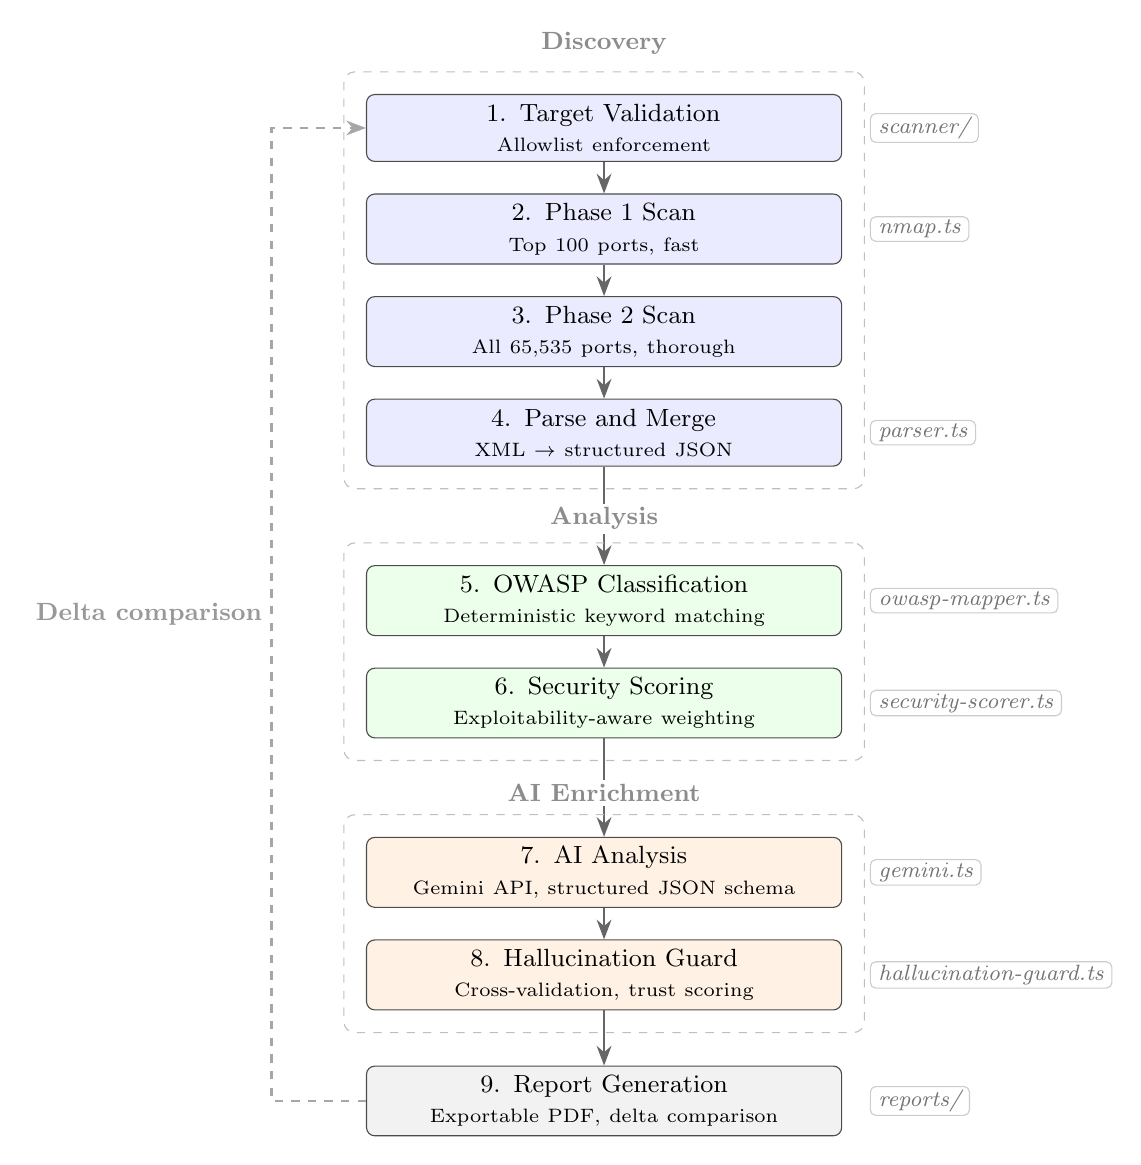
\begin{tikzpicture}[
    % Node styles
    stage/.style={
        rectangle,
        rounded corners=3pt,
        draw=black!70,
        fill=blue!8,
        text width=5.8cm,
        minimum height=0.85cm,
        align=center,
        font=\small
    },
    module/.style={
        draw=black!20,
        rounded corners=2pt,
        fill=white,
        inner xsep=3pt,
        inner ysep=1.2pt,
        font=\footnotesize\itshape,
        text=black!55
    },
    arrow/.style={
        -{Stealth[length=2.5mm]},
        thick,
        black!60
    },
    phaselabel/.style={
        font=\scriptsize\bfseries,
        text=black!50,
        anchor=east
    },
    groupbox/.style={
        rectangle,
        rounded corners=4pt,
        draw=black!25,
        dashed,
        inner sep=8pt
    },
    grouplabel/.style={
        fill=white,
        inner xsep=4pt,
        inner ysep=1.5pt,
        font=\small\bfseries,
        text=black!45
    },
    deltalabel/.style={
        fill=white,
        inner xsep=3pt,
        inner ysep=1.2pt,
        font=\small\bfseries,
        text=black!45
    }
]

% --- Nodes (top to bottom) ---

% Discovery group
\node[stage] (validate) {1. Target Validation \\ {\scriptsize Allowlist enforcement}};
\node[module, right=0.35cm of validate.east, anchor=west] {scanner/};

\node[stage, below=0.4cm of validate] (phase1) {2. Phase 1 Scan \\ {\scriptsize Top 100 ports, fast}};
\node[module, right=0.35cm of phase1.east, anchor=west] {nmap.ts};

\node[stage, below=0.4cm of phase1] (phase2) {3. Phase 2 Scan \\ {\scriptsize All 65{,}535 ports, thorough}};

\node[stage, below=0.4cm of phase2] (parse) {4. Parse and Merge \\ {\scriptsize XML $\rightarrow$ structured JSON}};
\node[module, right=0.35cm of parse.east, anchor=west] {parser.ts};

% Analysis group
\node[stage, below=1.25cm of parse, fill=green!8] (owasp) {5. OWASP Classification \\ {\scriptsize Deterministic keyword matching}};
\node[module, right=0.35cm of owasp.east, anchor=west] {owasp-mapper.ts};

\node[stage, below=0.4cm of owasp, fill=green!8] (score) {6. Security Scoring \\ {\scriptsize Exploitability-aware weighting}};
\node[module, right=0.35cm of score.east, anchor=west] {security-scorer.ts};

% AI group
\node[stage, below=1.25cm of score, fill=orange!10] (ai) {7. AI Analysis \\ {\scriptsize Gemini API, structured JSON schema}};
\node[module, right=0.35cm of ai.east, anchor=west] {gemini.ts};

\node[stage, below=0.4cm of ai, fill=orange!10] (guard) {8. Hallucination Guard \\ {\scriptsize Cross-validation, trust scoring}};
\node[module, right=0.35cm of guard.east, anchor=west] {hallucination-guard.ts};

% Output
\node[stage, below=0.7cm of guard, fill=gray!10] (report) {9. Report Generation \\ {\scriptsize Exportable PDF, delta comparison}};
\node[module, right=0.35cm of report.east, anchor=west] {reports/};

% --- Arrows ---
\draw[arrow] (validate) -- (phase1);
\draw[arrow] (phase1) -- (phase2);
\draw[arrow] (phase2) -- (parse);
\draw[arrow] (parse) -- (owasp);
\draw[arrow] (owasp) -- (score);
\draw[arrow] (score) -- (ai);
\draw[arrow] (ai) -- (guard);
\draw[arrow] (guard) -- (report);

% --- Group boxes ---
\node[groupbox, fit=(validate)(phase2)(parse), inner sep=8pt] (discbox) {};
\node[grouplabel, above=0.16cm of discbox.north, anchor=south] {Discovery};

\node[groupbox, fit=(owasp)(score), inner sep=8pt] (analbox) {};
\node[grouplabel, above=0.10cm of analbox.north, anchor=south] {Analysis};

\node[groupbox, fit=(ai)(guard), inner sep=8pt] (aibox) {};
\node[grouplabel, above=0.10cm of aibox.north, anchor=south] {AI Enrichment};

% --- Feedback arrow for delta comparison ---
\draw[-{Stealth[length=2.5mm]}, thick, black!35, dashed]
    (report.west) -- ++(-1.2,0) |- node[deltalabel, pos=0.25, left, text=black!40] {Delta comparison}
    (validate.west);

\end{tikzpicture}
\caption{PurpleTeam Suite pipeline architecture. Each stage is implemented as an independent module. The dashed feedback arrow represents the iterative scan-remediate-rescan lifecycle supported by the delta comparison system.}
\label{fig:pipeline}
\end{figure}
 where you want the figure,
% or paste the figure environment directly into Chapter 3.
% ============================================================

\begin{figure}[H]
\centering
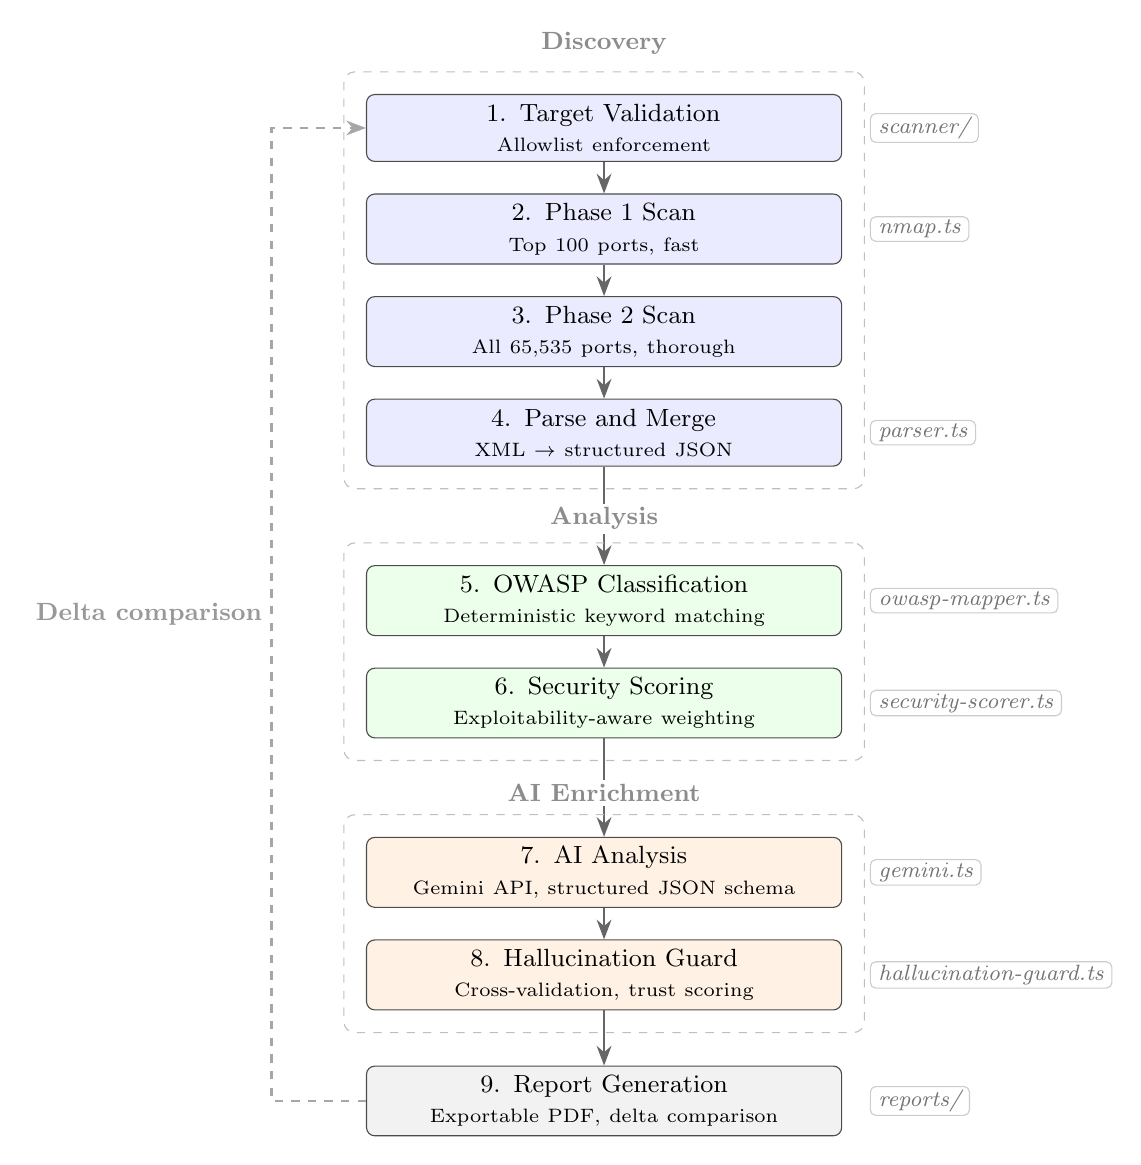
\begin{tikzpicture}[
    % Node styles
    stage/.style={
        rectangle,
        rounded corners=3pt,
        draw=black!70,
        fill=blue!8,
        text width=5.8cm,
        minimum height=0.85cm,
        align=center,
        font=\small
    },
    module/.style={
        draw=black!20,
        rounded corners=2pt,
        fill=white,
        inner xsep=3pt,
        inner ysep=1.2pt,
        font=\footnotesize\itshape,
        text=black!55
    },
    arrow/.style={
        -{Stealth[length=2.5mm]},
        thick,
        black!60
    },
    phaselabel/.style={
        font=\scriptsize\bfseries,
        text=black!50,
        anchor=east
    },
    groupbox/.style={
        rectangle,
        rounded corners=4pt,
        draw=black!25,
        dashed,
        inner sep=8pt
    },
    grouplabel/.style={
        fill=white,
        inner xsep=4pt,
        inner ysep=1.5pt,
        font=\small\bfseries,
        text=black!45
    },
    deltalabel/.style={
        fill=white,
        inner xsep=3pt,
        inner ysep=1.2pt,
        font=\small\bfseries,
        text=black!45
    }
]

% --- Nodes (top to bottom) ---

% Discovery group
\node[stage] (validate) {1. Target Validation \\ {\scriptsize Allowlist enforcement}};
\node[module, right=0.35cm of validate.east, anchor=west] {scanner/};

\node[stage, below=0.4cm of validate] (phase1) {2. Phase 1 Scan \\ {\scriptsize Top 100 ports, fast}};
\node[module, right=0.35cm of phase1.east, anchor=west] {nmap.ts};

\node[stage, below=0.4cm of phase1] (phase2) {3. Phase 2 Scan \\ {\scriptsize All 65{,}535 ports, thorough}};

\node[stage, below=0.4cm of phase2] (parse) {4. Parse and Merge \\ {\scriptsize XML $\rightarrow$ structured JSON}};
\node[module, right=0.35cm of parse.east, anchor=west] {parser.ts};

% Analysis group
\node[stage, below=1.25cm of parse, fill=green!8] (owasp) {5. OWASP Classification \\ {\scriptsize Deterministic keyword matching}};
\node[module, right=0.35cm of owasp.east, anchor=west] {owasp-mapper.ts};

\node[stage, below=0.4cm of owasp, fill=green!8] (score) {6. Security Scoring \\ {\scriptsize Exploitability-aware weighting}};
\node[module, right=0.35cm of score.east, anchor=west] {security-scorer.ts};

% AI group
\node[stage, below=1.25cm of score, fill=orange!10] (ai) {7. AI Analysis \\ {\scriptsize Gemini API, structured JSON schema}};
\node[module, right=0.35cm of ai.east, anchor=west] {gemini.ts};

\node[stage, below=0.4cm of ai, fill=orange!10] (guard) {8. Hallucination Guard \\ {\scriptsize Cross-validation, trust scoring}};
\node[module, right=0.35cm of guard.east, anchor=west] {hallucination-guard.ts};

% Output
\node[stage, below=0.7cm of guard, fill=gray!10] (report) {9. Report Generation \\ {\scriptsize Exportable PDF, delta comparison}};
\node[module, right=0.35cm of report.east, anchor=west] {reports/};

% --- Arrows ---
\draw[arrow] (validate) -- (phase1);
\draw[arrow] (phase1) -- (phase2);
\draw[arrow] (phase2) -- (parse);
\draw[arrow] (parse) -- (owasp);
\draw[arrow] (owasp) -- (score);
\draw[arrow] (score) -- (ai);
\draw[arrow] (ai) -- (guard);
\draw[arrow] (guard) -- (report);

% --- Group boxes ---
\node[groupbox, fit=(validate)(phase2)(parse), inner sep=8pt] (discbox) {};
\node[grouplabel, above=0.16cm of discbox.north, anchor=south] {Discovery};

\node[groupbox, fit=(owasp)(score), inner sep=8pt] (analbox) {};
\node[grouplabel, above=0.10cm of analbox.north, anchor=south] {Analysis};

\node[groupbox, fit=(ai)(guard), inner sep=8pt] (aibox) {};
\node[grouplabel, above=0.10cm of aibox.north, anchor=south] {AI Enrichment};

% --- Feedback arrow for delta comparison ---
\draw[-{Stealth[length=2.5mm]}, thick, black!35, dashed]
    (report.west) -- ++(-1.2,0) |- node[deltalabel, pos=0.25, left, text=black!40] {Delta comparison}
    (validate.west);

\end{tikzpicture}
\caption{PurpleTeam Suite pipeline architecture. Each stage is implemented as an independent module. The dashed feedback arrow represents the iterative scan-remediate-rescan lifecycle supported by the delta comparison system.}
\label{fig:pipeline}
\end{figure}
 where you want the figure,
% or paste the figure environment directly into Chapter 3.
% ============================================================

\begin{figure}[H]
\centering
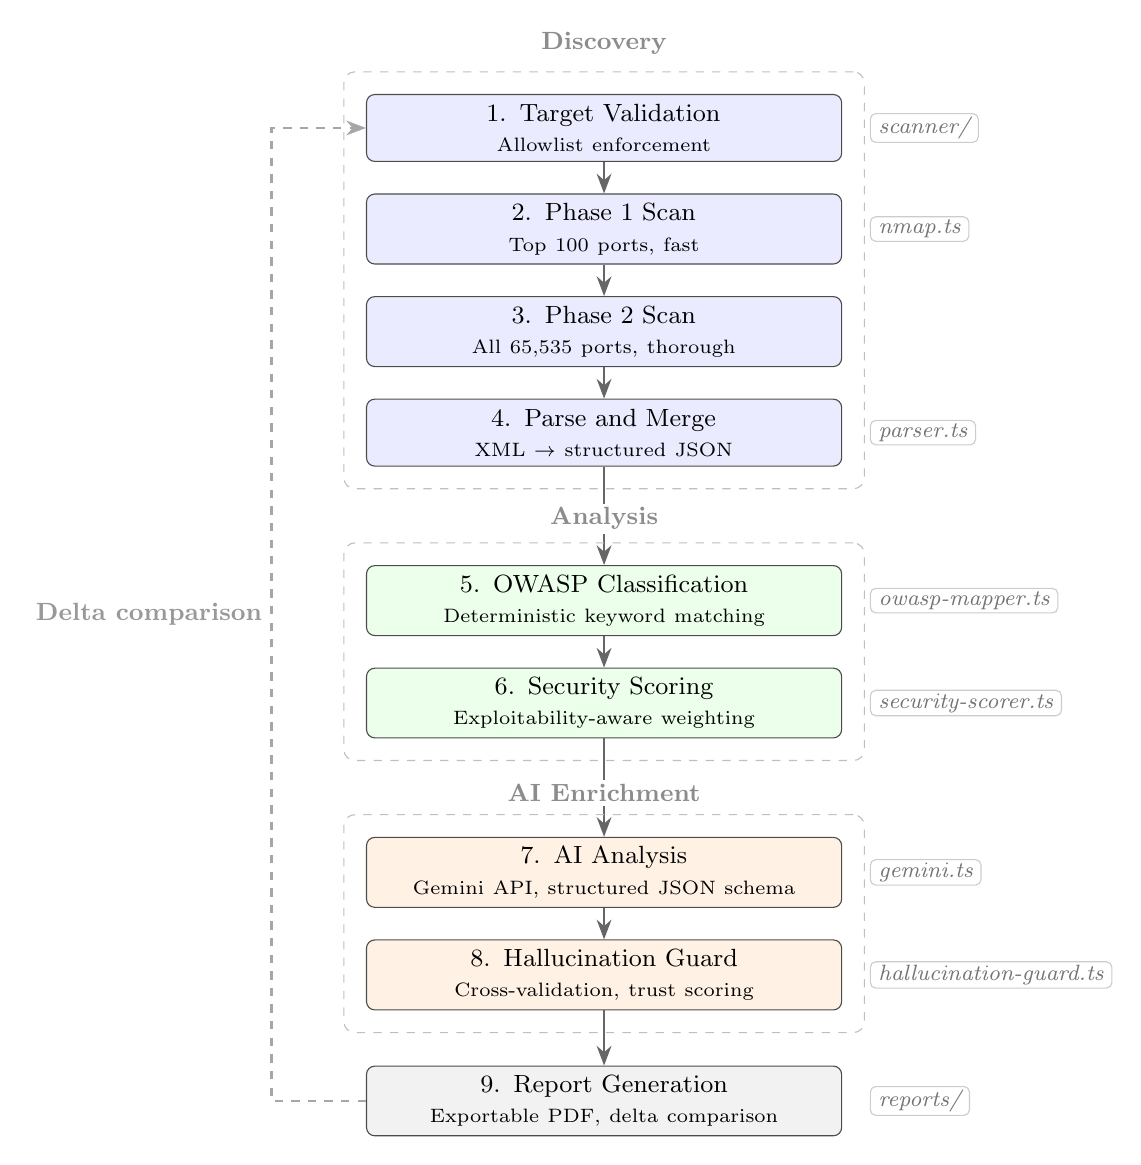
\begin{tikzpicture}[
    % Node styles
    stage/.style={
        rectangle,
        rounded corners=3pt,
        draw=black!70,
        fill=blue!8,
        text width=5.8cm,
        minimum height=0.85cm,
        align=center,
        font=\small
    },
    module/.style={
        draw=black!20,
        rounded corners=2pt,
        fill=white,
        inner xsep=3pt,
        inner ysep=1.2pt,
        font=\footnotesize\itshape,
        text=black!55
    },
    arrow/.style={
        -{Stealth[length=2.5mm]},
        thick,
        black!60
    },
    phaselabel/.style={
        font=\scriptsize\bfseries,
        text=black!50,
        anchor=east
    },
    groupbox/.style={
        rectangle,
        rounded corners=4pt,
        draw=black!25,
        dashed,
        inner sep=8pt
    },
    grouplabel/.style={
        fill=white,
        inner xsep=4pt,
        inner ysep=1.5pt,
        font=\small\bfseries,
        text=black!45
    },
    deltalabel/.style={
        fill=white,
        inner xsep=3pt,
        inner ysep=1.2pt,
        font=\small\bfseries,
        text=black!45
    }
]

% --- Nodes (top to bottom) ---

% Discovery group
\node[stage] (validate) {1. Target Validation \\ {\scriptsize Allowlist enforcement}};
\node[module, right=0.35cm of validate.east, anchor=west] {scanner/};

\node[stage, below=0.4cm of validate] (phase1) {2. Phase 1 Scan \\ {\scriptsize Top 100 ports, fast}};
\node[module, right=0.35cm of phase1.east, anchor=west] {nmap.ts};

\node[stage, below=0.4cm of phase1] (phase2) {3. Phase 2 Scan \\ {\scriptsize All 65{,}535 ports, thorough}};

\node[stage, below=0.4cm of phase2] (parse) {4. Parse and Merge \\ {\scriptsize XML $\rightarrow$ structured JSON}};
\node[module, right=0.35cm of parse.east, anchor=west] {parser.ts};

% Analysis group
\node[stage, below=1.25cm of parse, fill=green!8] (owasp) {5. OWASP Classification \\ {\scriptsize Deterministic keyword matching}};
\node[module, right=0.35cm of owasp.east, anchor=west] {owasp-mapper.ts};

\node[stage, below=0.4cm of owasp, fill=green!8] (score) {6. Security Scoring \\ {\scriptsize Exploitability-aware weighting}};
\node[module, right=0.35cm of score.east, anchor=west] {security-scorer.ts};

% AI group
\node[stage, below=1.25cm of score, fill=orange!10] (ai) {7. AI Analysis \\ {\scriptsize Gemini API, structured JSON schema}};
\node[module, right=0.35cm of ai.east, anchor=west] {gemini.ts};

\node[stage, below=0.4cm of ai, fill=orange!10] (guard) {8. Hallucination Guard \\ {\scriptsize Cross-validation, trust scoring}};
\node[module, right=0.35cm of guard.east, anchor=west] {hallucination-guard.ts};

% Output
\node[stage, below=0.7cm of guard, fill=gray!10] (report) {9. Report Generation \\ {\scriptsize Exportable PDF, delta comparison}};
\node[module, right=0.35cm of report.east, anchor=west] {reports/};

% --- Arrows ---
\draw[arrow] (validate) -- (phase1);
\draw[arrow] (phase1) -- (phase2);
\draw[arrow] (phase2) -- (parse);
\draw[arrow] (parse) -- (owasp);
\draw[arrow] (owasp) -- (score);
\draw[arrow] (score) -- (ai);
\draw[arrow] (ai) -- (guard);
\draw[arrow] (guard) -- (report);

% --- Group boxes ---
\node[groupbox, fit=(validate)(phase2)(parse), inner sep=8pt] (discbox) {};
\node[grouplabel, above=0.16cm of discbox.north, anchor=south] {Discovery};

\node[groupbox, fit=(owasp)(score), inner sep=8pt] (analbox) {};
\node[grouplabel, above=0.10cm of analbox.north, anchor=south] {Analysis};

\node[groupbox, fit=(ai)(guard), inner sep=8pt] (aibox) {};
\node[grouplabel, above=0.10cm of aibox.north, anchor=south] {AI Enrichment};

% --- Feedback arrow for delta comparison ---
\draw[-{Stealth[length=2.5mm]}, thick, black!35, dashed]
    (report.west) -- ++(-1.2,0) |- node[deltalabel, pos=0.25, left, text=black!40] {Delta comparison}
    (validate.west);

\end{tikzpicture}
\caption{PurpleTeam Suite pipeline architecture. Each stage is implemented as an independent module. The dashed feedback arrow represents the iterative scan-remediate-rescan lifecycle supported by the delta comparison system.}
\label{fig:pipeline}
\end{figure}
 % TikZ pipeline figure



\subsection{Scanning and Detection}

The scanner module orchestrates Nmap as an external child process, using a two-phase progressive design to balance responsiveness against coverage~\cite{chalvatzis2019}: Phase~1 scans the top 100 ports and returns early results within approximately two to four minutes, while Phase~2 runs a full 65,535-port scan in the background, with results merged and deduplicated after both phases complete. The parser additionally injects post-processing detections for missing security headers and absent HTTPS, extending coverage into configuration-level findings that Nmap's scripting engine does not natively report.

\begin{figure}[htbp]
\centering
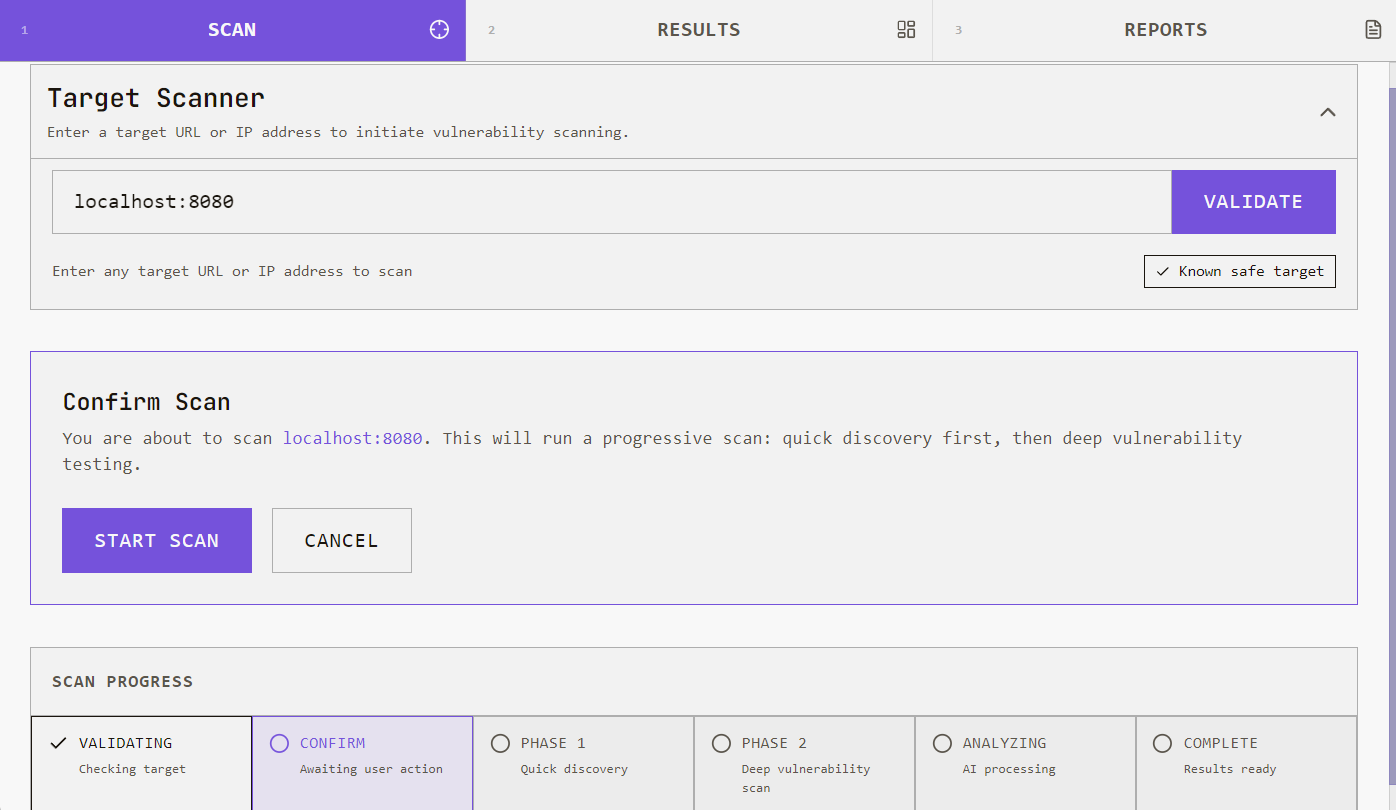
\includegraphics[width=0.95\textwidth]{NewFigures/scantarget.png}
\caption{Scan target input interface with allowlist validation. The six-step progress stepper is visible prior to scan execution.}
\label{fig:scan-target}
\end{figure}

\subsection{Classification and Scoring}

The classification layer uses a deterministic keyword matcher to map each vulnerability to OWASP Top~10 categories; it runs before the AI component, establishing a ground-truth classification that the hallucination guard later cross-references. The scoring model addresses the limitations of static CVSS-based prioritisation~\cite{howland2023,jacobs2023} by applying four contextual multipliers: port exposure weighting, service exposure, an authentication weakness multiplier, and a flat TLS absence penalty. All multipliers are defined as named constants and are fully deterministic; a runtime feature toggle allows contextual weighting to be disabled for ablation testing. A flat +10 remediation bonus is applied when AI analysis completes successfully, reflecting full pipeline execution. Figure~\ref{fig:dashboard} presents the dashboard view of a completed scan.

\begin{figure}[htbp]
\centering
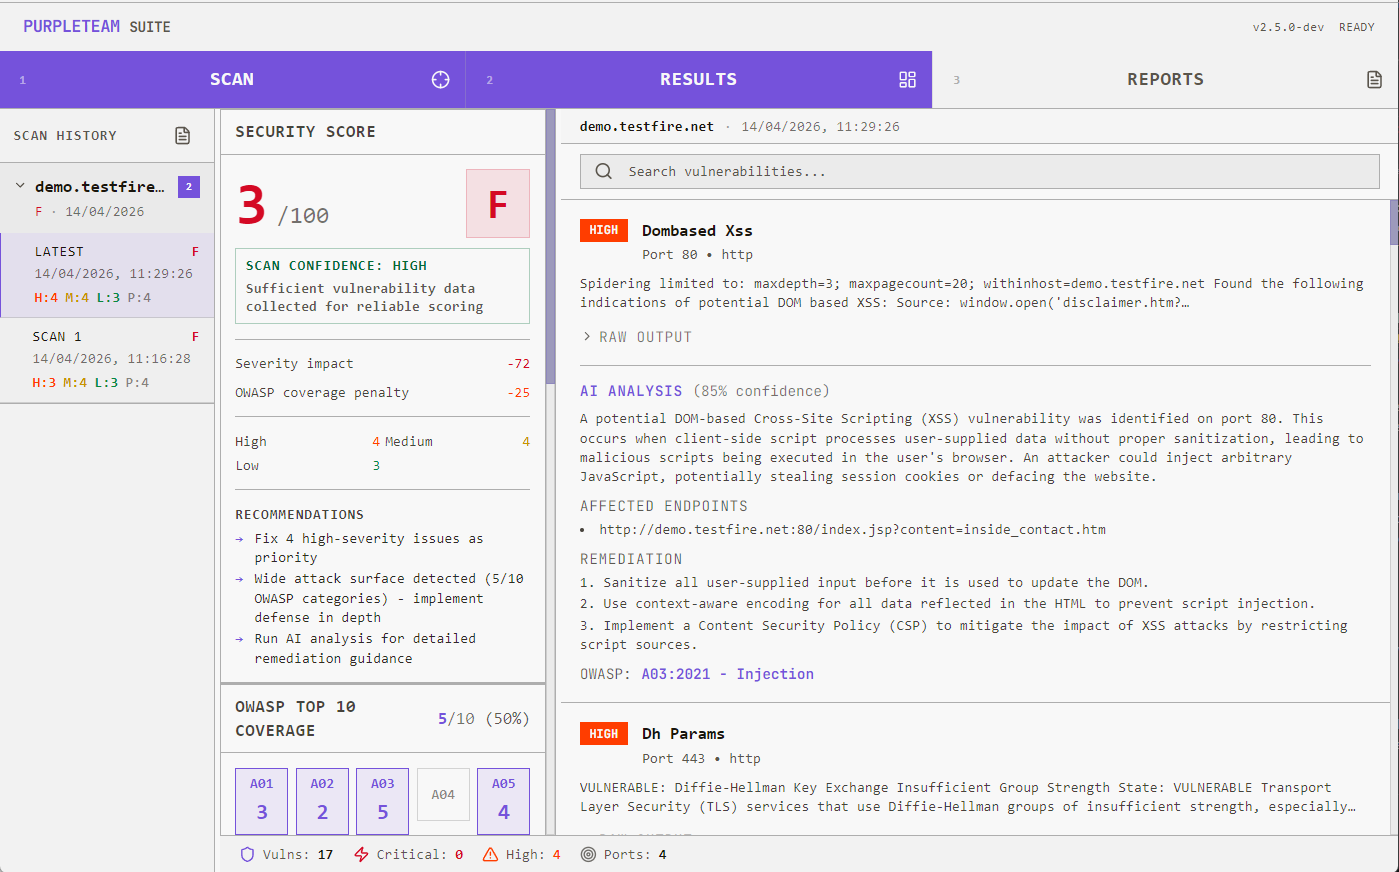
\includegraphics[width=0.95\textwidth]{NewFigures/Purpleteam suite dashboard.png}
\caption{PurpleTeam Suite dashboard displaying security score with exploitability-aware weighting, OWASP Top 10 coverage matrix and prioritised vulnerability table.}
\label{fig:dashboard}
\end{figure}

\subsection{AI Integration and Hallucination Control}

The LLM component sends compressed vulnerability data to Google Gemini under structured JSON output enforcement and a constrained response schema, ensuring the model analyses only what the scanner found~\cite{lin2025,chen2024}. The hallucination guard cross-references AI OWASP assignments against the deterministic mapper's classifications, verifies that cited CVE identifiers appear in the scan data, and computes a weighted trust score that penalises fabricated CVEs most heavily, OWASP disagreements moderately, and confidence mismatches least. Trust scores are clamped to the 0--100 range and persisted longitudinally to enable reliability tracking across scans. Figure~\ref{fig:ai-detail} illustrates the AI-generated analysis for a single vulnerability.

\begin{figure}[htbp]
\centering
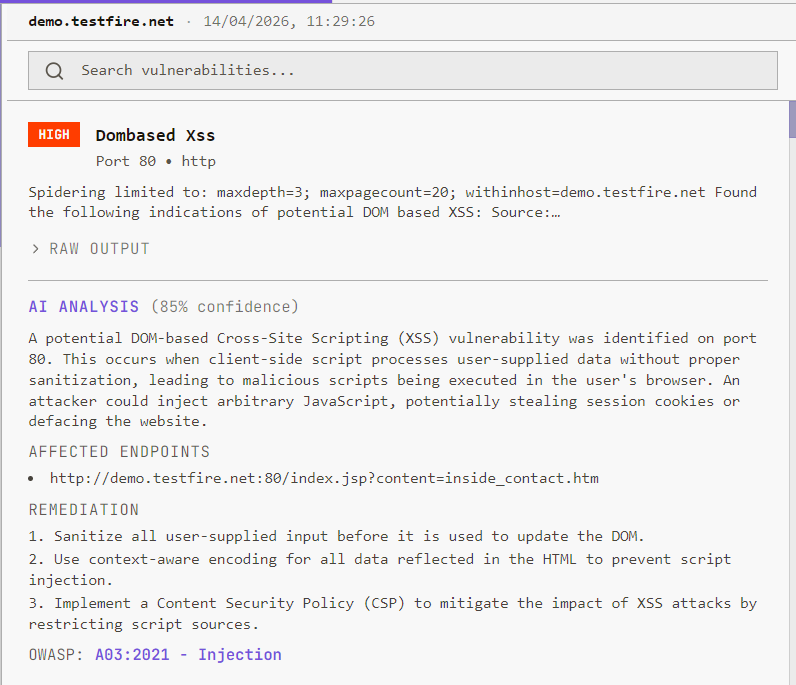
\includegraphics[width=0.95\textwidth]{NewFigures/AI-GeneratedAnalysis.png}
\caption{AI-generated vulnerability analysis showing plain-English summary, severity justification and structured remediation steps. The hallucination guard trust indicators are displayed alongside each finding.}
\label{fig:ai-detail}
\end{figure}

\subsection{Lifecycle Support}
\label{sec:lifecycle}

The delta comparison module closes the purple-team lifecycle loop identified as a gap in the literature~\cite{holm2025} by fingerprinting vulnerabilities across consecutive scans and classifying each finding as resolved, persisting or newly introduced, with score changes, OWASP coverage shifts and directional indicators presented in both the dashboard and an exportable report. Figure~\ref{fig:delta} shows the in-app comparison view and the exported report used to evidence lifecycle impact in Section~\ref{sec:phase4-results}.

\begin{figure}[H]
\centering
\captionsetup{skip=2pt}
\captionsetup[subfigure]{font=small, justification=centering, singlelinecheck=false, aboveskip=1pt, belowskip=0pt}
\begin{subfigure}[t]{\textwidth}
\centering
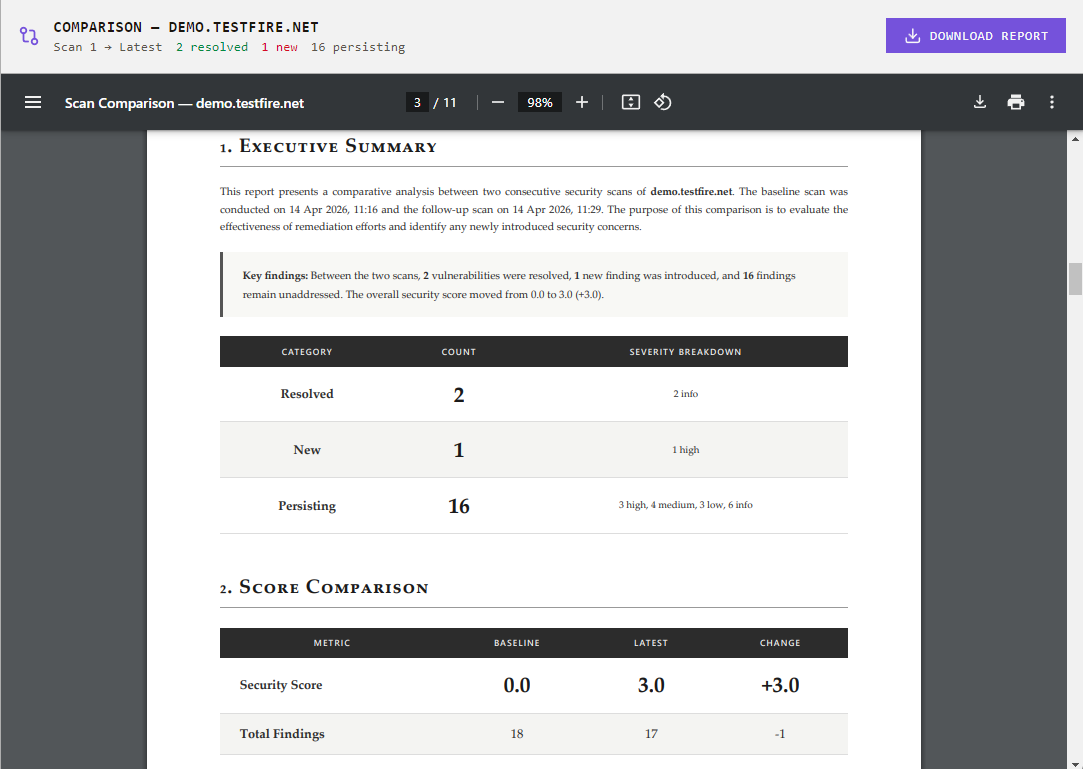
\includegraphics[width=\textwidth,height=0.38\textheight,keepaspectratio]{NewFigures/comparison.png}
\caption{In-app comparison report executive summary view (toggle-driven delta example).}
\end{subfigure}

\vspace{-0.2em}

\begin{subfigure}[t]{\textwidth}
\centering
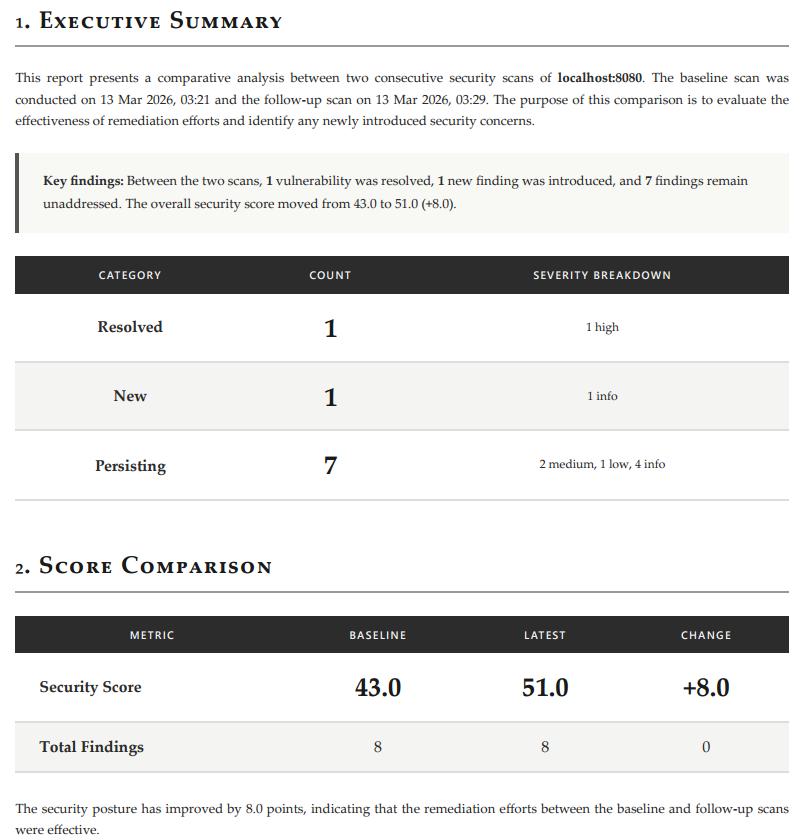
\includegraphics[width=\textwidth,height=0.34\textheight,keepaspectratio,trim=8 24 8 24,clip]{product/delta-comparison}
\caption{Exported localhost comparison report excerpt showing a +8 score improvement after local target changes; this screenshot predates the definitive lifecycle evaluation reported in Section~4.5.}
\end{subfigure}

\caption{Delta comparison outputs in PurpleTeam Suite, showing both the application report interface and the exported report evidence used in lifecycle evaluation.}
\label{fig:delta}
\end{figure}

\subsection{Implementation Environment}
\label{sec:implementation}

Table~\ref{tab:techstack} and Table~\ref{tab:keylibraries} summarise the technology stack and key dependencies; selection rationale and architectural justification are provided in Appendix~C.

% --- Both tables placed together so LaTeX floats them as a block ---

\begin{table}[htbp]
\centering
\caption{Core technology stack and selection rationale.}
\label{tab:techstack}
\small
\renewcommand{\arraystretch}{1.45}
\setlength{\tabcolsep}{5pt}
\begin{tabularx}{\textwidth}{
    >{\raggedright\arraybackslash}p{2.2cm}
    >{\raggedright\arraybackslash}p{2.8cm}
    >{\raggedright\arraybackslash}X
}
\toprule
\rowcolor{headerblue}
\textcolor{headertext}{\textbf{Layer}} &
\textcolor{headertext}{\textbf{Technology}} &
\textcolor{headertext}{\textbf{Justification}} \\
\midrule
\rowcolor{rowlight}
Desktop framework &
Electron &
Compiles to native executables for Windows, macOS and Linux from a single TypeScript codebase; provides secure IPC isolation between renderer and main processes, ensuring the UI cannot directly access the file system or spawn scanning tools \\

\rowcolor{rowwhite}
Frontend &
React 19, TypeScript &
Component-based UI architecture with static type checking, reducing runtime errors in security-critical data handling \\

\rowcolor{rowlight}
Styling &
Tailwind CSS &
Utility-first approach enabling rapid, consistent UI development without external stylesheet dependencies \\

\rowcolor{rowwhite}
Build tooling &
Vite &
Sub-second hot module replacement during development; native TypeScript and JSX support without additional transpilation configuration \\

\rowcolor{rowlight}
Scanning &
Nmap (external) &
Industry-standard network scanner validated for automated pipeline use~\cite{singh2024}; spawned as a child process to maintain separation from the application runtime \\

\rowcolor{rowwhite}
XML parsing &
xml2js &
Converts Nmap's XML output into traversable JavaScript objects; mature library with established handling of Nmap's output schema \\

\rowcolor{rowlight}
AI provider &
Google Gemini 2.5 Flash &
Structured JSON output mode, low-latency inference, configurable temperature, and sufficient context window for batch vulnerability analysis \\

\rowcolor{rowwhite}
Routing &
React Router &
Client-side navigation between scan, dashboard and reports views without full page reloads \\

\rowcolor{rowlight}
State management &
Custom singleton store &
Lightweight in-memory store avoiding external state library overhead; persists across page navigation through React hooks subscription \\

\rowcolor{rowwhite}
PDF generation &
jsPDF (programmatic) &
Enables server-side PDF generation within the Electron main process without browser print dependencies \\
\bottomrule
\end{tabularx}
\renewcommand{\arraystretch}{1.0}
\end{table}

\begin{table}[htbp]
\centering
\caption{Key library dependencies and pipeline integration points.}
\label{tab:keylibraries}
\small
\renewcommand{\arraystretch}{1.45}
\setlength{\tabcolsep}{5pt}
\begin{tabularx}{\textwidth}{
    >{\raggedright\arraybackslash}p{2.8cm}
    >{\raggedright\arraybackslash}p{2.0cm}
    >{\raggedright\arraybackslash}X
}
\toprule
\rowcolor{headerblue}
\textcolor{headertext}{\textbf{Library}} &
\textcolor{headertext}{\textbf{Pipeline Stage}} &
\textcolor{headertext}{\textbf{Role}} \\
\midrule
\rowcolor{rowlight}
\texttt{xml2js} &
Parse (Stage 3) &
Parses Nmap XML into typed JSON; handles nested script output and multi-valued fields \\

\rowcolor{rowwhite}
\texttt{@google/generative-ai} &
AI Analysis (Stage 8) &
Official Gemini SDK; provides structured output mode, temperature control, token limits and retry configuration \\

\rowcolor{rowlight}
\texttt{jspdf} &
Report (Stage 10) &
Generates multi-page PDF reports programmatically with custom layouts, tables and embedded score visualisations \\

\rowcolor{rowwhite}
\texttt{electron} &
Application shell &
Main and renderer process management, IPC bridge, context isolation, system dialog access for file export \\

\rowcolor{rowlight}
\texttt{react-router-dom} &
UI navigation &
Declarative routing between scan, dashboard and reports pages \\

\rowcolor{rowwhite}
\texttt{dotenv} &
Configuration &
Loads Gemini API keys from \texttt{.env} file, keeping credentials outside the codebase and version control \\
\bottomrule
\end{tabularx}
\renewcommand{\arraystretch}{1.0}
\end{table}

\FloatBarrier

\clearpage
\section{Evaluation Framework}
\label{sec:evaluation-framework}

The evaluation is structured across five phases, each producing quantitative data against defined metrics across five authorised test targets representing a range of technology stacks, deployment models and vulnerability profiles. Phase~1 establishes baseline consistency; Phase~2 compares flat versus contextual weighting; Phase~3 performs per-component ablation on Mutillidae using a runtime feature toggle system; Phase~4 demonstrates the iterative lifecycle on the controlled testbed; and Phase~5 accumulates longitudinal hallucination guard metrics across all targets. The five phases are summarised in Table~\ref{tab:eval-framework}.

% ============================================================
%  evaluation-diagram.tex
%  Five-phase evaluation framework — styled matrix figure
%  % ============================================================
%  evaluation-diagram.tex
%  Five-phase evaluation framework — styled matrix figure
%  % ============================================================
%  evaluation-diagram.tex
%  Five-phase evaluation framework — styled matrix figure
%  \input{evaluation-diagram} at the end of Section 3.3,
%  after the closing metrics paragraph and before \section{Limitations}
% ============================================================

\begin{table}[p]
\centering
\small
\renewcommand{\arraystretch}{1.6}
\setlength{\tabcolsep}{6pt}
\begin{tabularx}{\textwidth}{
  >{\centering\arraybackslash}p{0.9cm}
  >{\centering\arraybackslash}p{2.8cm}
  >{\raggedright\arraybackslash}p{3.2cm}
  >{\raggedright\arraybackslash}p{3.0cm}
  >{\raggedright\arraybackslash}X
}
\toprule
\rowcolor{headerblue}
\textcolor{headertext}{\textbf{\#}} &
\textcolor{headertext}{\textbf{Phase}} &
\textcolor{headertext}{\textbf{Targets \& Config.}} &
\textcolor{headertext}{\textbf{Method}} &
\textcolor{headertext}{\textbf{Key Output Metrics}} \\
\midrule

\rowcolor{rowlight}
\textbf{1} &
Baseline Consistency &
All five targets\newline Weighting: \textbf{OFF}\newline 2 runs per target &
Run the full pipeline twice per target. Verify identical inputs produce identical outputs. &
Baseline scores $B_1$,~$B_2$~$\cdot$~Scan consistency rate~$\cdot$~OWASP coverage breadth \\

\rowcolor{rowwhite}
\textbf{2} &
Exploitability-Aware Scoring Impact &
All five targets\newline Weighting: \textbf{ON}\newline 1 run per target &
Re-run with contextual weighting enabled. Compare adjusted scores against Phase~1 baselines. &
Score delta $\Delta E$ vs Phase~1~$\cdot$~Per-multiplier breakdown~$\cdot$~Adjusted vs flat score table \\

\rowcolor{rowlight}
\textbf{3} &
Ablation Testing &
localhost only\newline Weighting: toggle\newline No re-scan required &
Disable one component per run and reprocess the same scan data. Components: OWASP mapper, AI analysis, hallucination guard, contextual weighting. &
Per-component score and classification delta~$\cdot$~Ablation table across four toggle conditions \\

\rowcolor{rowwhite}
\textbf{4} &
Lifecycle Demonstration &
localhost only\newline Weighting: \textbf{ON}\newline Scan~$\to$~fix~$\to$~rescan &
Remediate a defined vulnerability subset, rescan, and generate a delta comparison report. &
Score improvement $\Delta S$~$\cdot$~Resolved and persisting counts~$\cdot$~OWASP coverage contraction \\

\rowcolor{rowlight}
\textbf{5} &
Longitudinal Hallucination Reliability &
All five targets\newline Weighting: \textbf{ON}\newline Accumulated across scans &
Accumulate hallucination guard metrics across all targets and scans to produce a longitudinal reliability dataset. &
Trust score~$\cdot$~OWASP disagreement rate~$\cdot$~Confidence mismatch rate~$\cdot$~Fabricated CVE count \\

\bottomrule
\end{tabularx}
\renewcommand{\arraystretch}{1.0}
\caption{Five-phase evaluation framework with target configurations, methods and key output metrics.}
\label{tab:eval-framework}
\end{table} at the end of Section 3.3,
%  after the closing metrics paragraph and before \section{Limitations}
% ============================================================

\begin{table}[p]
\centering
\small
\renewcommand{\arraystretch}{1.6}
\setlength{\tabcolsep}{6pt}
\begin{tabularx}{\textwidth}{
  >{\centering\arraybackslash}p{0.9cm}
  >{\centering\arraybackslash}p{2.8cm}
  >{\raggedright\arraybackslash}p{3.2cm}
  >{\raggedright\arraybackslash}p{3.0cm}
  >{\raggedright\arraybackslash}X
}
\toprule
\rowcolor{headerblue}
\textcolor{headertext}{\textbf{\#}} &
\textcolor{headertext}{\textbf{Phase}} &
\textcolor{headertext}{\textbf{Targets \& Config.}} &
\textcolor{headertext}{\textbf{Method}} &
\textcolor{headertext}{\textbf{Key Output Metrics}} \\
\midrule

\rowcolor{rowlight}
\textbf{1} &
Baseline Consistency &
All five targets\newline Weighting: \textbf{OFF}\newline 2 runs per target &
Run the full pipeline twice per target. Verify identical inputs produce identical outputs. &
Baseline scores $B_1$,~$B_2$~$\cdot$~Scan consistency rate~$\cdot$~OWASP coverage breadth \\

\rowcolor{rowwhite}
\textbf{2} &
Exploitability-Aware Scoring Impact &
All five targets\newline Weighting: \textbf{ON}\newline 1 run per target &
Re-run with contextual weighting enabled. Compare adjusted scores against Phase~1 baselines. &
Score delta $\Delta E$ vs Phase~1~$\cdot$~Per-multiplier breakdown~$\cdot$~Adjusted vs flat score table \\

\rowcolor{rowlight}
\textbf{3} &
Ablation Testing &
localhost only\newline Weighting: toggle\newline No re-scan required &
Disable one component per run and reprocess the same scan data. Components: OWASP mapper, AI analysis, hallucination guard, contextual weighting. &
Per-component score and classification delta~$\cdot$~Ablation table across four toggle conditions \\

\rowcolor{rowwhite}
\textbf{4} &
Lifecycle Demonstration &
localhost only\newline Weighting: \textbf{ON}\newline Scan~$\to$~fix~$\to$~rescan &
Remediate a defined vulnerability subset, rescan, and generate a delta comparison report. &
Score improvement $\Delta S$~$\cdot$~Resolved and persisting counts~$\cdot$~OWASP coverage contraction \\

\rowcolor{rowlight}
\textbf{5} &
Longitudinal Hallucination Reliability &
All five targets\newline Weighting: \textbf{ON}\newline Accumulated across scans &
Accumulate hallucination guard metrics across all targets and scans to produce a longitudinal reliability dataset. &
Trust score~$\cdot$~OWASP disagreement rate~$\cdot$~Confidence mismatch rate~$\cdot$~Fabricated CVE count \\

\bottomrule
\end{tabularx}
\renewcommand{\arraystretch}{1.0}
\caption{Five-phase evaluation framework with target configurations, methods and key output metrics.}
\label{tab:eval-framework}
\end{table} at the end of Section 3.3,
%  after the closing metrics paragraph and before \section{Limitations}
% ============================================================

\begin{table}[p]
\centering
\small
\renewcommand{\arraystretch}{1.6}
\setlength{\tabcolsep}{6pt}
\begin{tabularx}{\textwidth}{
  >{\centering\arraybackslash}p{0.9cm}
  >{\centering\arraybackslash}p{2.8cm}
  >{\raggedright\arraybackslash}p{3.2cm}
  >{\raggedright\arraybackslash}p{3.0cm}
  >{\raggedright\arraybackslash}X
}
\toprule
\rowcolor{headerblue}
\textcolor{headertext}{\textbf{\#}} &
\textcolor{headertext}{\textbf{Phase}} &
\textcolor{headertext}{\textbf{Targets \& Config.}} &
\textcolor{headertext}{\textbf{Method}} &
\textcolor{headertext}{\textbf{Key Output Metrics}} \\
\midrule

\rowcolor{rowlight}
\textbf{1} &
Baseline Consistency &
All five targets\newline Weighting: \textbf{OFF}\newline 2 runs per target &
Run the full pipeline twice per target. Verify identical inputs produce identical outputs. &
Baseline scores $B_1$,~$B_2$~$\cdot$~Scan consistency rate~$\cdot$~OWASP coverage breadth \\

\rowcolor{rowwhite}
\textbf{2} &
Exploitability-Aware Scoring Impact &
All five targets\newline Weighting: \textbf{ON}\newline 1 run per target &
Re-run with contextual weighting enabled. Compare adjusted scores against Phase~1 baselines. &
Score delta $\Delta E$ vs Phase~1~$\cdot$~Per-multiplier breakdown~$\cdot$~Adjusted vs flat score table \\

\rowcolor{rowlight}
\textbf{3} &
Ablation Testing &
localhost only\newline Weighting: toggle\newline No re-scan required &
Disable one component per run and reprocess the same scan data. Components: OWASP mapper, AI analysis, hallucination guard, contextual weighting. &
Per-component score and classification delta~$\cdot$~Ablation table across four toggle conditions \\

\rowcolor{rowwhite}
\textbf{4} &
Lifecycle Demonstration &
localhost only\newline Weighting: \textbf{ON}\newline Scan~$\to$~fix~$\to$~rescan &
Remediate a defined vulnerability subset, rescan, and generate a delta comparison report. &
Score improvement $\Delta S$~$\cdot$~Resolved and persisting counts~$\cdot$~OWASP coverage contraction \\

\rowcolor{rowlight}
\textbf{5} &
Longitudinal Hallucination Reliability &
All five targets\newline Weighting: \textbf{ON}\newline Accumulated across scans &
Accumulate hallucination guard metrics across all targets and scans to produce a longitudinal reliability dataset. &
Trust score~$\cdot$~OWASP disagreement rate~$\cdot$~Confidence mismatch rate~$\cdot$~Fabricated CVE count \\

\bottomrule
\end{tabularx}
\renewcommand{\arraystretch}{1.0}
\caption{Five-phase evaluation framework with target configurations, methods and key output metrics.}
\label{tab:eval-framework}
\end{table}
\FloatBarrier

\section{Limitations and Ethical Considerations}
\label{sec:limitations-ethics}

The system carries several acknowledged limitations. The target set is small,
comprising five authorised environments, which limits the generalisability of
evaluation findings. The AI component depends on a single LLM provider, and
model behaviour may differ across versions or alternative providers. The
contextual weighting multipliers were calibrated based on common exposure
patterns rather than empirical attack frequency data, and should be treated as
operationally reasonable defaults rather than statistically validated risk
weights.

The system performs active network scanning, which is regulated under the
Computer Misuse Act 1990. Accordingly, all scanning was restricted to
authorised targets through an enforced allowlist validation mechanism that
prevents scan execution against unapproved hosts. All testing was restricted to
the five authorised targets described in Section~\ref{sec:evaluation-framework}.
No live production systems were tested and no human participants or personal
data were involved. Ethical approval was granted by the project supervisor on
11~February 2026.

Only compressed vulnerability metadata is transmitted to the Gemini API. Raw
scan outputs, network topology data and sensitive system information are not
uploaded, limiting external data exposure to the minimum necessary for AI
analysis. The hallucination guard further ensures that AI-generated claims are
not presented to the user without deterministic cross-validation, reducing the
risk of acting on fabricated security advice. The application displays a legal
disclaimer regarding the implications of misuse, and responsible operation
requires explicit authorisation from the target owner.

\section{Summary}
This chapter established the methodological foundation for the evaluation that follows. The system is designed against seven traceable requirements, each mapped to a pipeline module and evaluation phase, with a runtime feature toggle system enabling controlled ablation without modifying the codebase. The five-phase evaluation framework covers baseline consistency, exploitability-aware scoring impact, per-feature contribution isolation, iterative lifecycle demonstration and longitudinal hallucination reliability. The system is feature-complete, and results are presented in Chapter~4.

\FloatBarrier
 
% ============================================================
% Chapter 4 — Analysis and Results
% ============================================================
\addtocontents{toc}{\protect\newpage}
\chapter{Analysis and Results}

% ─────────────────────────────────────────────
\section{Evaluation Design Overview}
\label{sec:evaluation-overview}

The evaluation was conducted according to the five-phase framework defined in Section~\ref{sec:evaluation-framework}. Table~\ref{tab:eval-targets} summarises the five authorised targets; Phases~1, 2 and~5 ran across all five, Phase~3 (ablation) was conducted on Mutillidae only, and Phase~4 (lifecycle delta) on the controlled testbed only, the sole target with researcher-controlled vulnerability state.

\begin{table}[H]
\centering
\caption{Evaluation targets and their roles within the five-phase framework.}
\label{tab:eval-targets}
\footnotesize
\renewcommand{\arraystretch}{1.45}
\setlength{\tabcolsep}{4pt}
\begin{tabularx}{\textwidth}{
  >{\raggedright\arraybackslash}p{3.8cm}
  >{\raggedright\arraybackslash}p{3.6cm}
  >{\raggedright\arraybackslash}X}
\toprule
\rowcolor{headerblue}
\textcolor{headertext}{\textbf{Label}} &
\textcolor{headertext}{\textbf{Address}} &
\textcolor{headertext}{\textbf{Type and Role}} \\
\midrule
\rowcolor{rowlight}
Mutillidae &
\texttt{localhost} (port~80) &
Local, OWASP Docker. Mutillidae~II running at Security Level~0, exposing
Apache, PHPMyAdmin, OpenLDAP and HTTPS across ports 80, 81, 82, 389 and 443.
Used for Phases~1, 2, 3 and~5. \\
\rowcolor{rowwhite}
Controlled Testbed &
\texttt{127.0.0.1:8080} &
Local, custom Node.js. Purpose-built application with 12 intentional
vulnerabilities across multiple OWASP categories. Sole target with
researcher-controlled vulnerability state. Used for Phases~1, 3 and~4. \\
\rowcolor{rowlight}
scanme.nmap.org &
\texttt{scanme.nmap.org} &
Public, Nmap Project. Explicitly authorised for port scanning, minimal service
exposure provides a clean external reference. Used for Phases~1 and~5. \\
\rowcolor{rowwhite}
testasp.vulnweb.com &
\texttt{testasp.vulnweb.com} &
Public, Acunetix test site (IIS/ASP/MSSQL). Technology profile distinct from
the local PHP targets. Used for Phases~1 and~5. \\
\rowcolor{rowlight}
demo.testfire.net &
\texttt{demo.testfire.net} &
Public, HCL/IBM banking app (IIS/ASP.NET). Deliberately vulnerable
financial-services attack surface. Used for Phases~1 and~5. \\
\bottomrule
\end{tabularx}
\renewcommand{\arraystretch}{1.0}
\end{table}

All scans were conducted on a Windows~11 workstation with Nmap~7.98 on the system PATH; the \texttt{featureToggles} snapshot persisted with each result ensures full configuration traceability.

% ─────────────────────────────────────────────
\section{Phase 1: Baseline Consistency and Reproducibility}
\label{sec:phase1-results}

Severity deduction scores range from 50 to 181 across the five targets, with four receiving an F grade and only testasp.vulnweb.com achieving a D; Mutillidae's 26 findings across all severity tiers justify its selection as the primary ablation target in subsequent phases (Table~\ref{tab:baseline-results}, Figure~\ref{fig:baseline-scores}). Four of the five targets achieved 4/10 OWASP category coverage with detections concentrated in A01, A02, A03 and A05, with demo.testfire.net reaching 5/10 by additionally triggering A07 detections consistent with its financial-application authentication endpoints (Table~\ref{tab:baseline-owasp}, Figure~\ref{fig:owasp-heatmap}).

% Baseline results table — one row per target
\begin{table}[H]
\centering
\caption{Phase~1 baseline scan results across all five evaluation targets (all feature toggles enabled).}
\label{tab:baseline-results}
\footnotesize
\renewcommand{\arraystretch}{1.45}
\setlength{\tabcolsep}{5pt}
\begin{tabularx}{\textwidth}{@{}
  >{\raggedright\arraybackslash}p{3.8cm}
  >{\centering\arraybackslash}p{1.1cm}
  >{\centering\arraybackslash}p{1.0cm}
  >{\centering\arraybackslash}p{0.8cm}
  >{\centering\arraybackslash}p{0.8cm}
  >{\centering\arraybackslash}p{0.8cm}
  >{\centering\arraybackslash}p{0.8cm}
  >{\centering\arraybackslash}p{0.8cm}
  >{\centering\arraybackslash}X @{}}
\toprule
\rowcolor{headerblue}
\textcolor{headertext}{\textbf{Target}} &
\textcolor{headertext}{\textbf{Sev.\ Ded.}} &
\textcolor{headertext}{\textbf{Grade}} &
\textcolor{headertext}{\textbf{Crit.}} &
\textcolor{headertext}{\textbf{High}} &
\textcolor{headertext}{\textbf{Med.}} &
\textcolor{headertext}{\textbf{Low}} &
\textcolor{headertext}{\textbf{Info}} &
\textcolor{headertext}{\textbf{Total}} \\
\midrule
\rowcolor{rowlight}
Mutillidae              & 181 & F & 2 & 5 & 4 & 3 & 12 & 26 \\
\rowcolor{rowwhite}
Controlled Testbed      & 77  & F & 2 & 3 & 2 & 0 & 8  & 15 \\
\rowcolor{rowlight}
scanme.nmap.org         & 91  & F & 2 & 1 & 1 & 1 & 1  & 6  \\
\rowcolor{rowwhite}
demo.testfire.net       & 96  & F & 3 & 4 & 3 & 0 & 8  & 18 \\
\rowcolor{rowlight}
testasp.vulnweb.com     & 50  & D & 2 & 1 & 1 & 1 & 0  & 5  \\
\bottomrule
\end{tabularx}
\renewcommand{\arraystretch}{1.0}
\end{table}

% OWASP distribution table — one row per target
\begin{table}[H]
\centering
\caption{OWASP Top~10 category distribution across baseline scans.}
\label{tab:baseline-owasp}
\footnotesize
\renewcommand{\arraystretch}{1.45}
\setlength{\tabcolsep}{3pt}
\begin{tabularx}{\textwidth}{@{}
  >{\raggedright\arraybackslash}p{3.2cm}
  >{\centering\arraybackslash}p{0.7cm}
  >{\centering\arraybackslash}p{0.7cm}
  >{\centering\arraybackslash}p{0.7cm}
  >{\centering\arraybackslash}p{0.7cm}
  >{\centering\arraybackslash}p{0.7cm}
  >{\centering\arraybackslash}p{0.7cm}
  >{\centering\arraybackslash}p{0.7cm}
  >{\centering\arraybackslash}p{0.7cm}
  >{\centering\arraybackslash}p{0.7cm}
  >{\centering\arraybackslash}p{0.7cm}
  >{\centering\arraybackslash}X @{}}
\toprule
\rowcolor{headerblue}
\textcolor{headertext}{\textbf{Target}} &
\textcolor{headertext}{\textbf{A01}} &
\textcolor{headertext}{\textbf{A02}} &
\textcolor{headertext}{\textbf{A03}} &
\textcolor{headertext}{\textbf{A04}} &
\textcolor{headertext}{\textbf{A05}} &
\textcolor{headertext}{\textbf{A06}} &
\textcolor{headertext}{\textbf{A07}} &
\textcolor{headertext}{\textbf{A08}} &
\textcolor{headertext}{\textbf{A09}} &
\textcolor{headertext}{\textbf{A10}} &
\textcolor{headertext}{\textbf{Cov.}} \\
\midrule
\rowcolor{rowlight}
Mutillidae              & 2 & 5 & 7 & 0 & 12 & 0 & 0 & 0 & 0 & 0 & 4/10 \\
\rowcolor{rowwhite}
Controlled Testbed      & 2 & 5 & 0 & 0 & 6  & 0 & 2 & 0 & 0 & 0 & 4/10 \\
\rowcolor{rowlight}
scanme.nmap.org         & 1 & 3 & 1 & 0 & 1  & 0 & 0 & 0 & 0 & 0 & 4/10 \\
\rowcolor{rowwhite}
demo.testfire.net       & 3 & 2 & 6 & 0 & 4  & 0 & 3 & 0 & 0 & 0 & 5/10 \\
\rowcolor{rowlight}
testasp.vulnweb.com     & 1 & 2 & 0 & 0 & 1  & 0 & 1 & 0 & 0 & 0 & 4/10 \\
\bottomrule
\end{tabularx}
\renewcommand{\arraystretch}{1.0}
\end{table}


\begin{figure}[H]
\centering
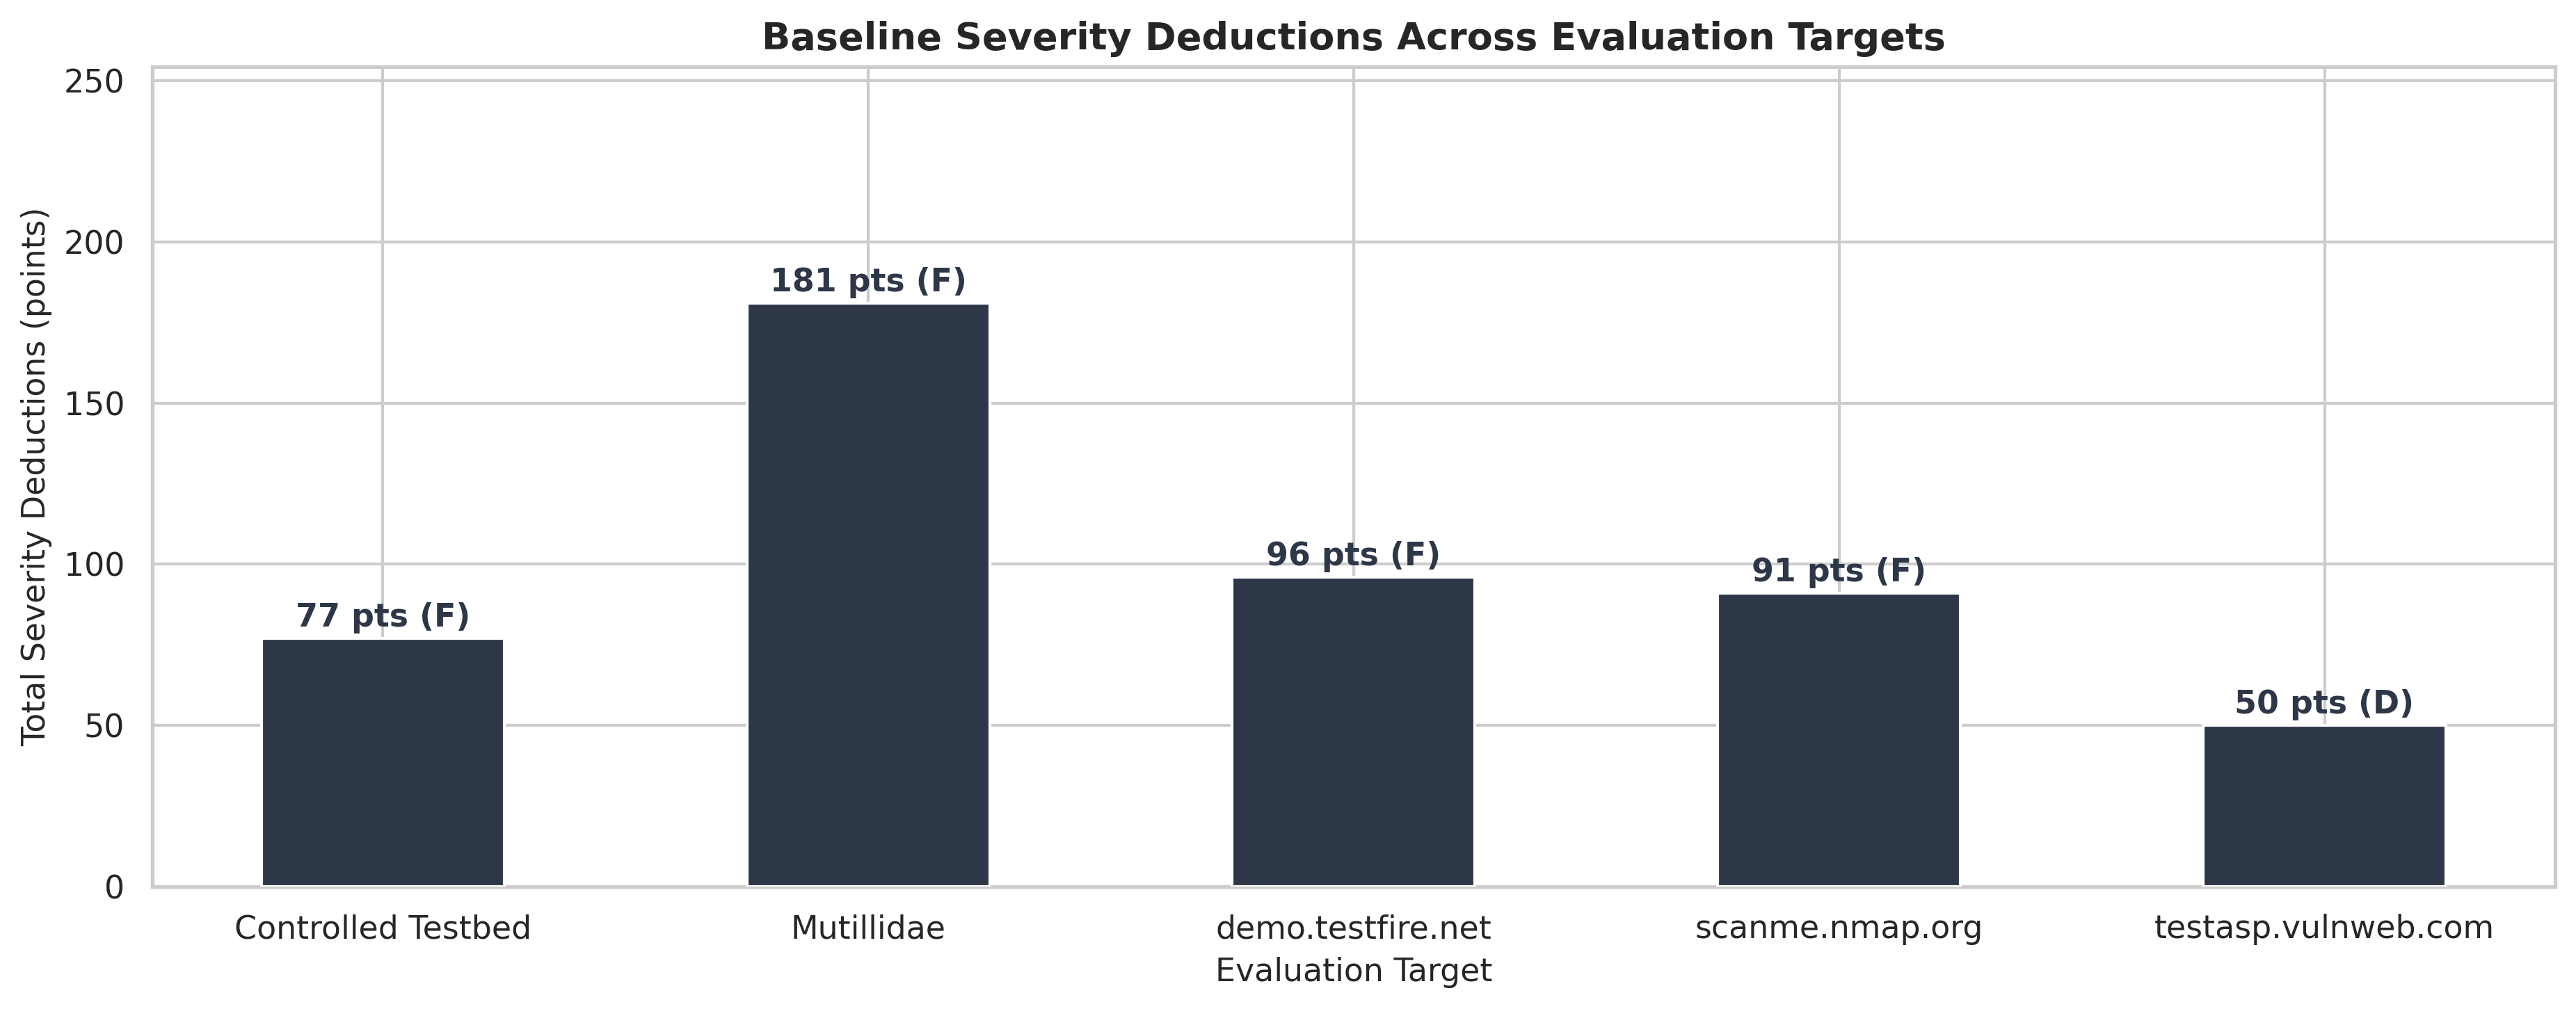
\includegraphics[width=\textwidth]{chapter4figures/fig_baseline_scores.png}
\caption{Severity deduction scores across all five baseline scans, illustrating the
  range from 50 (\mbox{testasp.vulnweb.com}) to 181 (Mutillidae).}
\label{fig:baseline-scores}
\end{figure}

\begin{figure}[H]
\centering
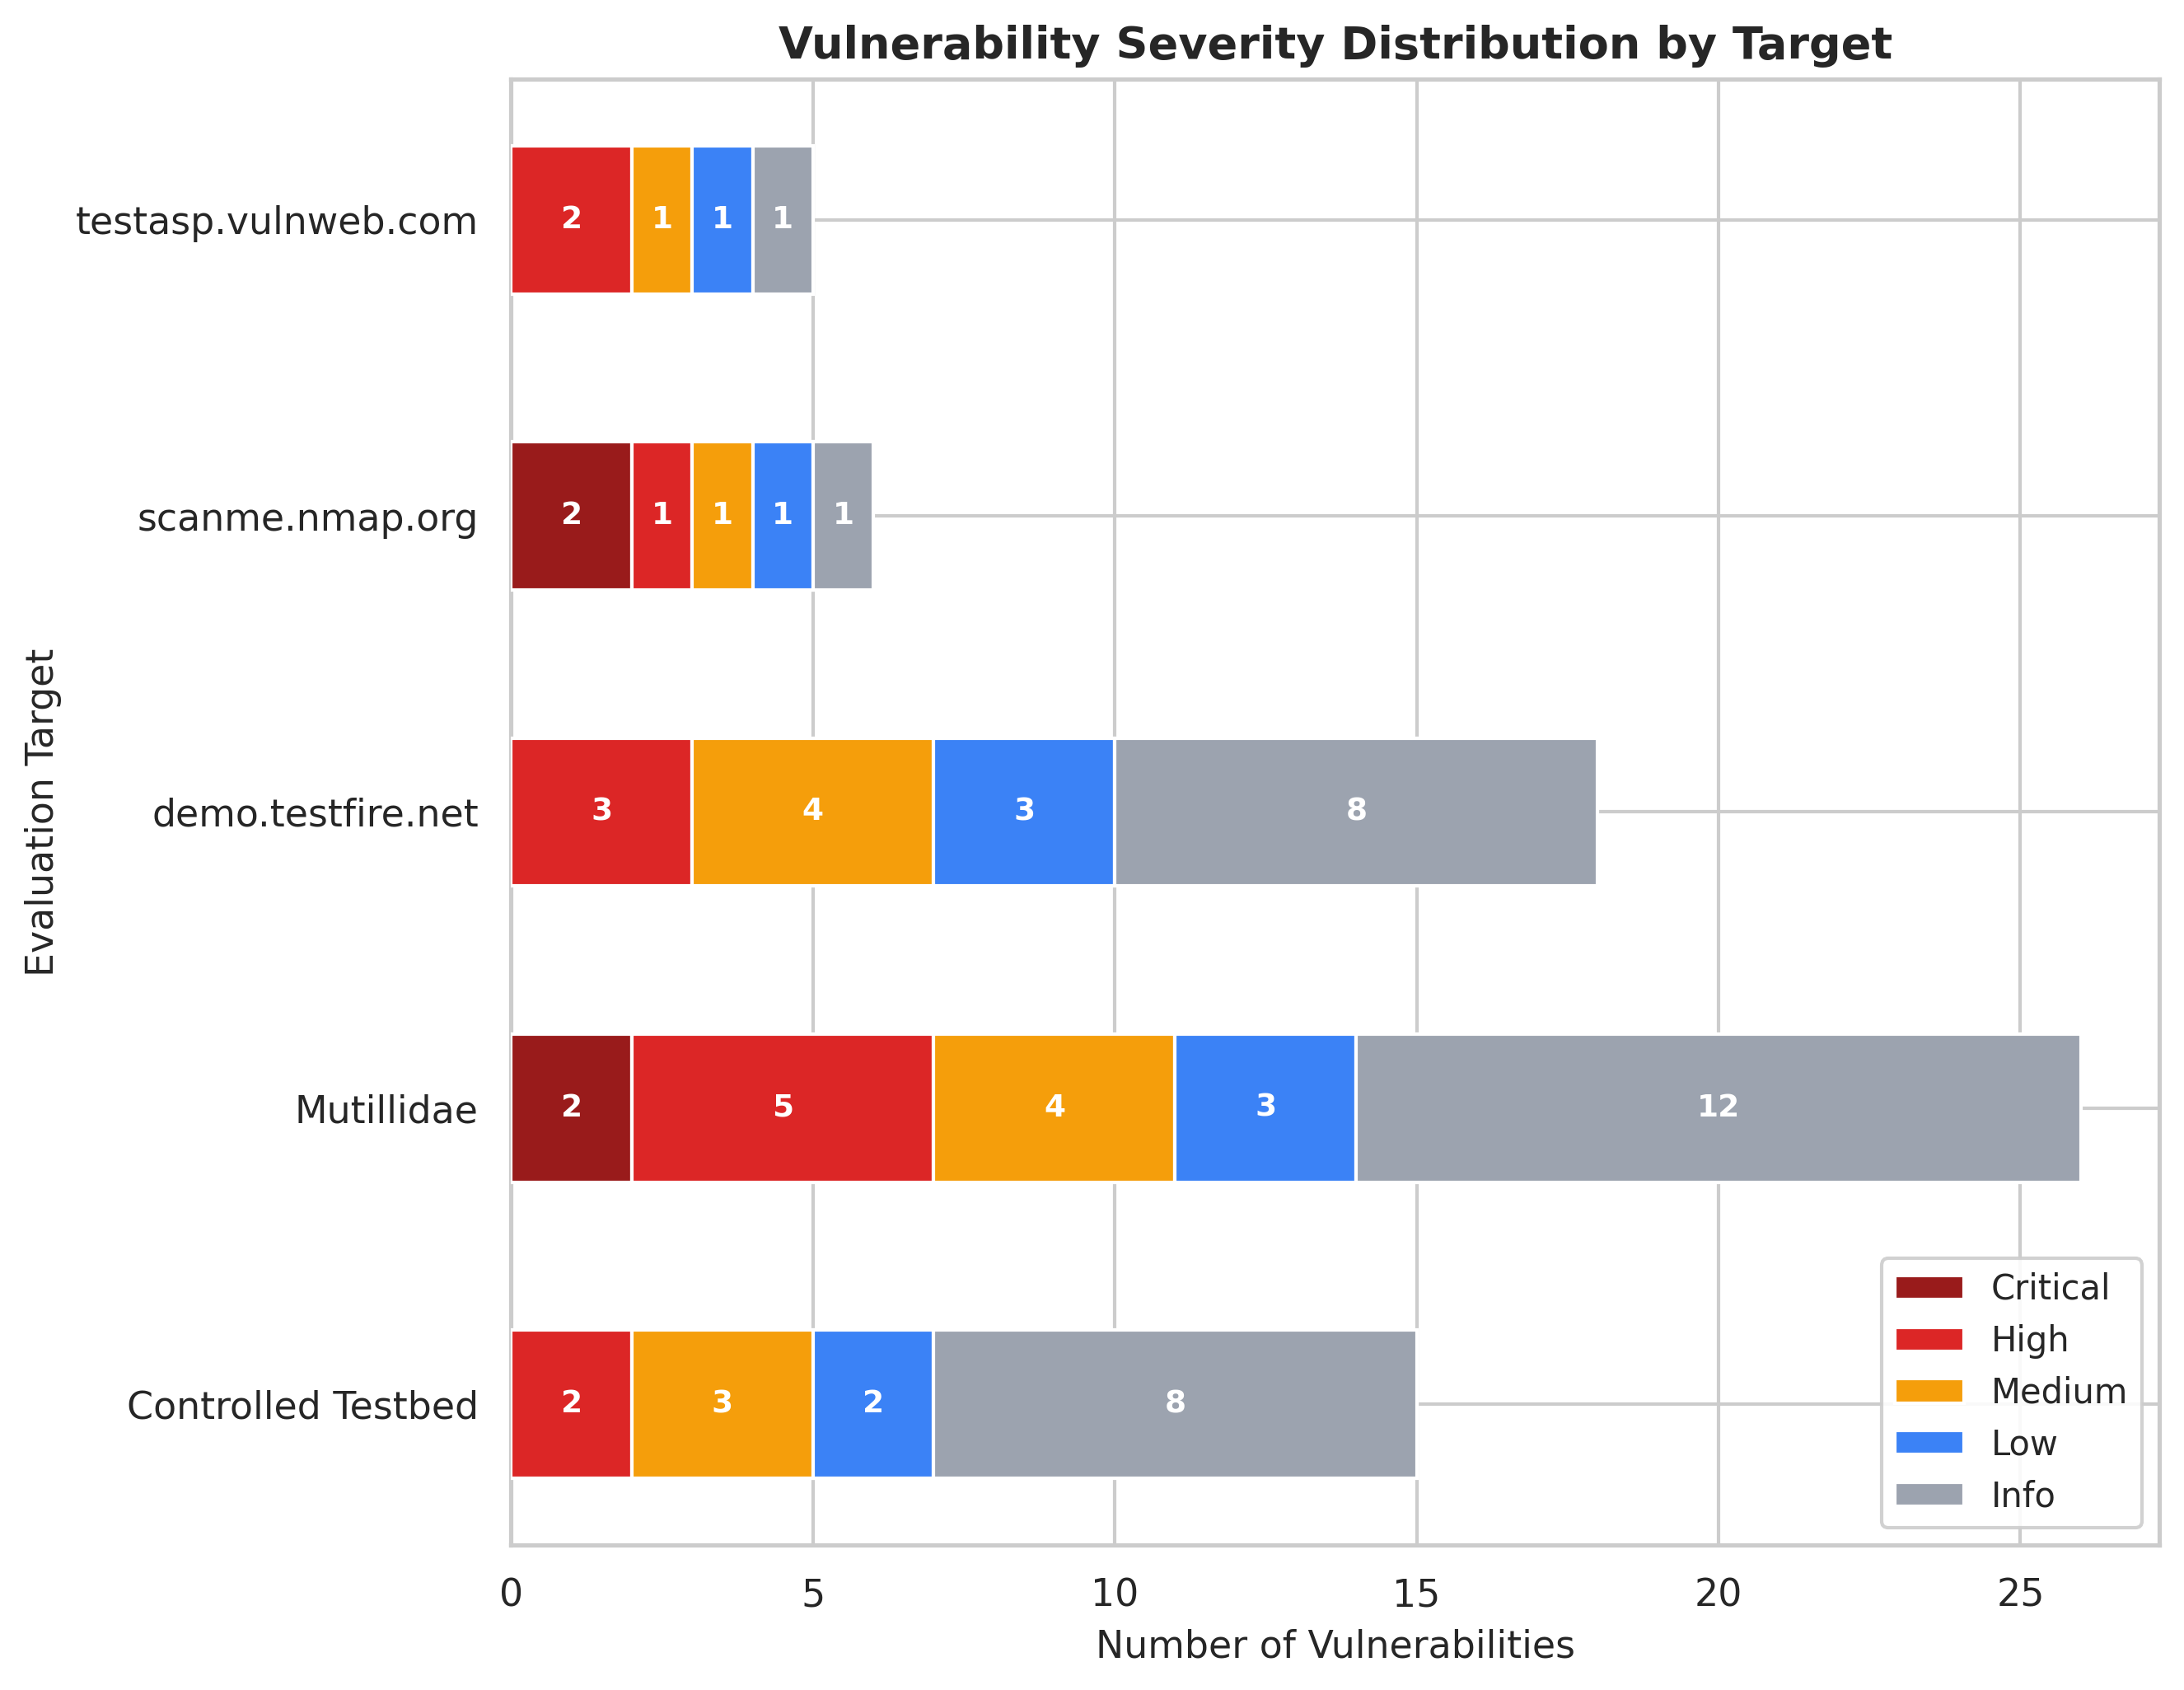
\includegraphics[width=\textwidth]{chapter4figures/fig_baseline_severity.png}
\caption{Severity distribution by target, showing the breakdown of Critical, High,
  Medium, Low and Informational findings across all five baseline scans.}
\label{fig:baseline-severity}
\end{figure}

\begin{figure}[H]
\centering
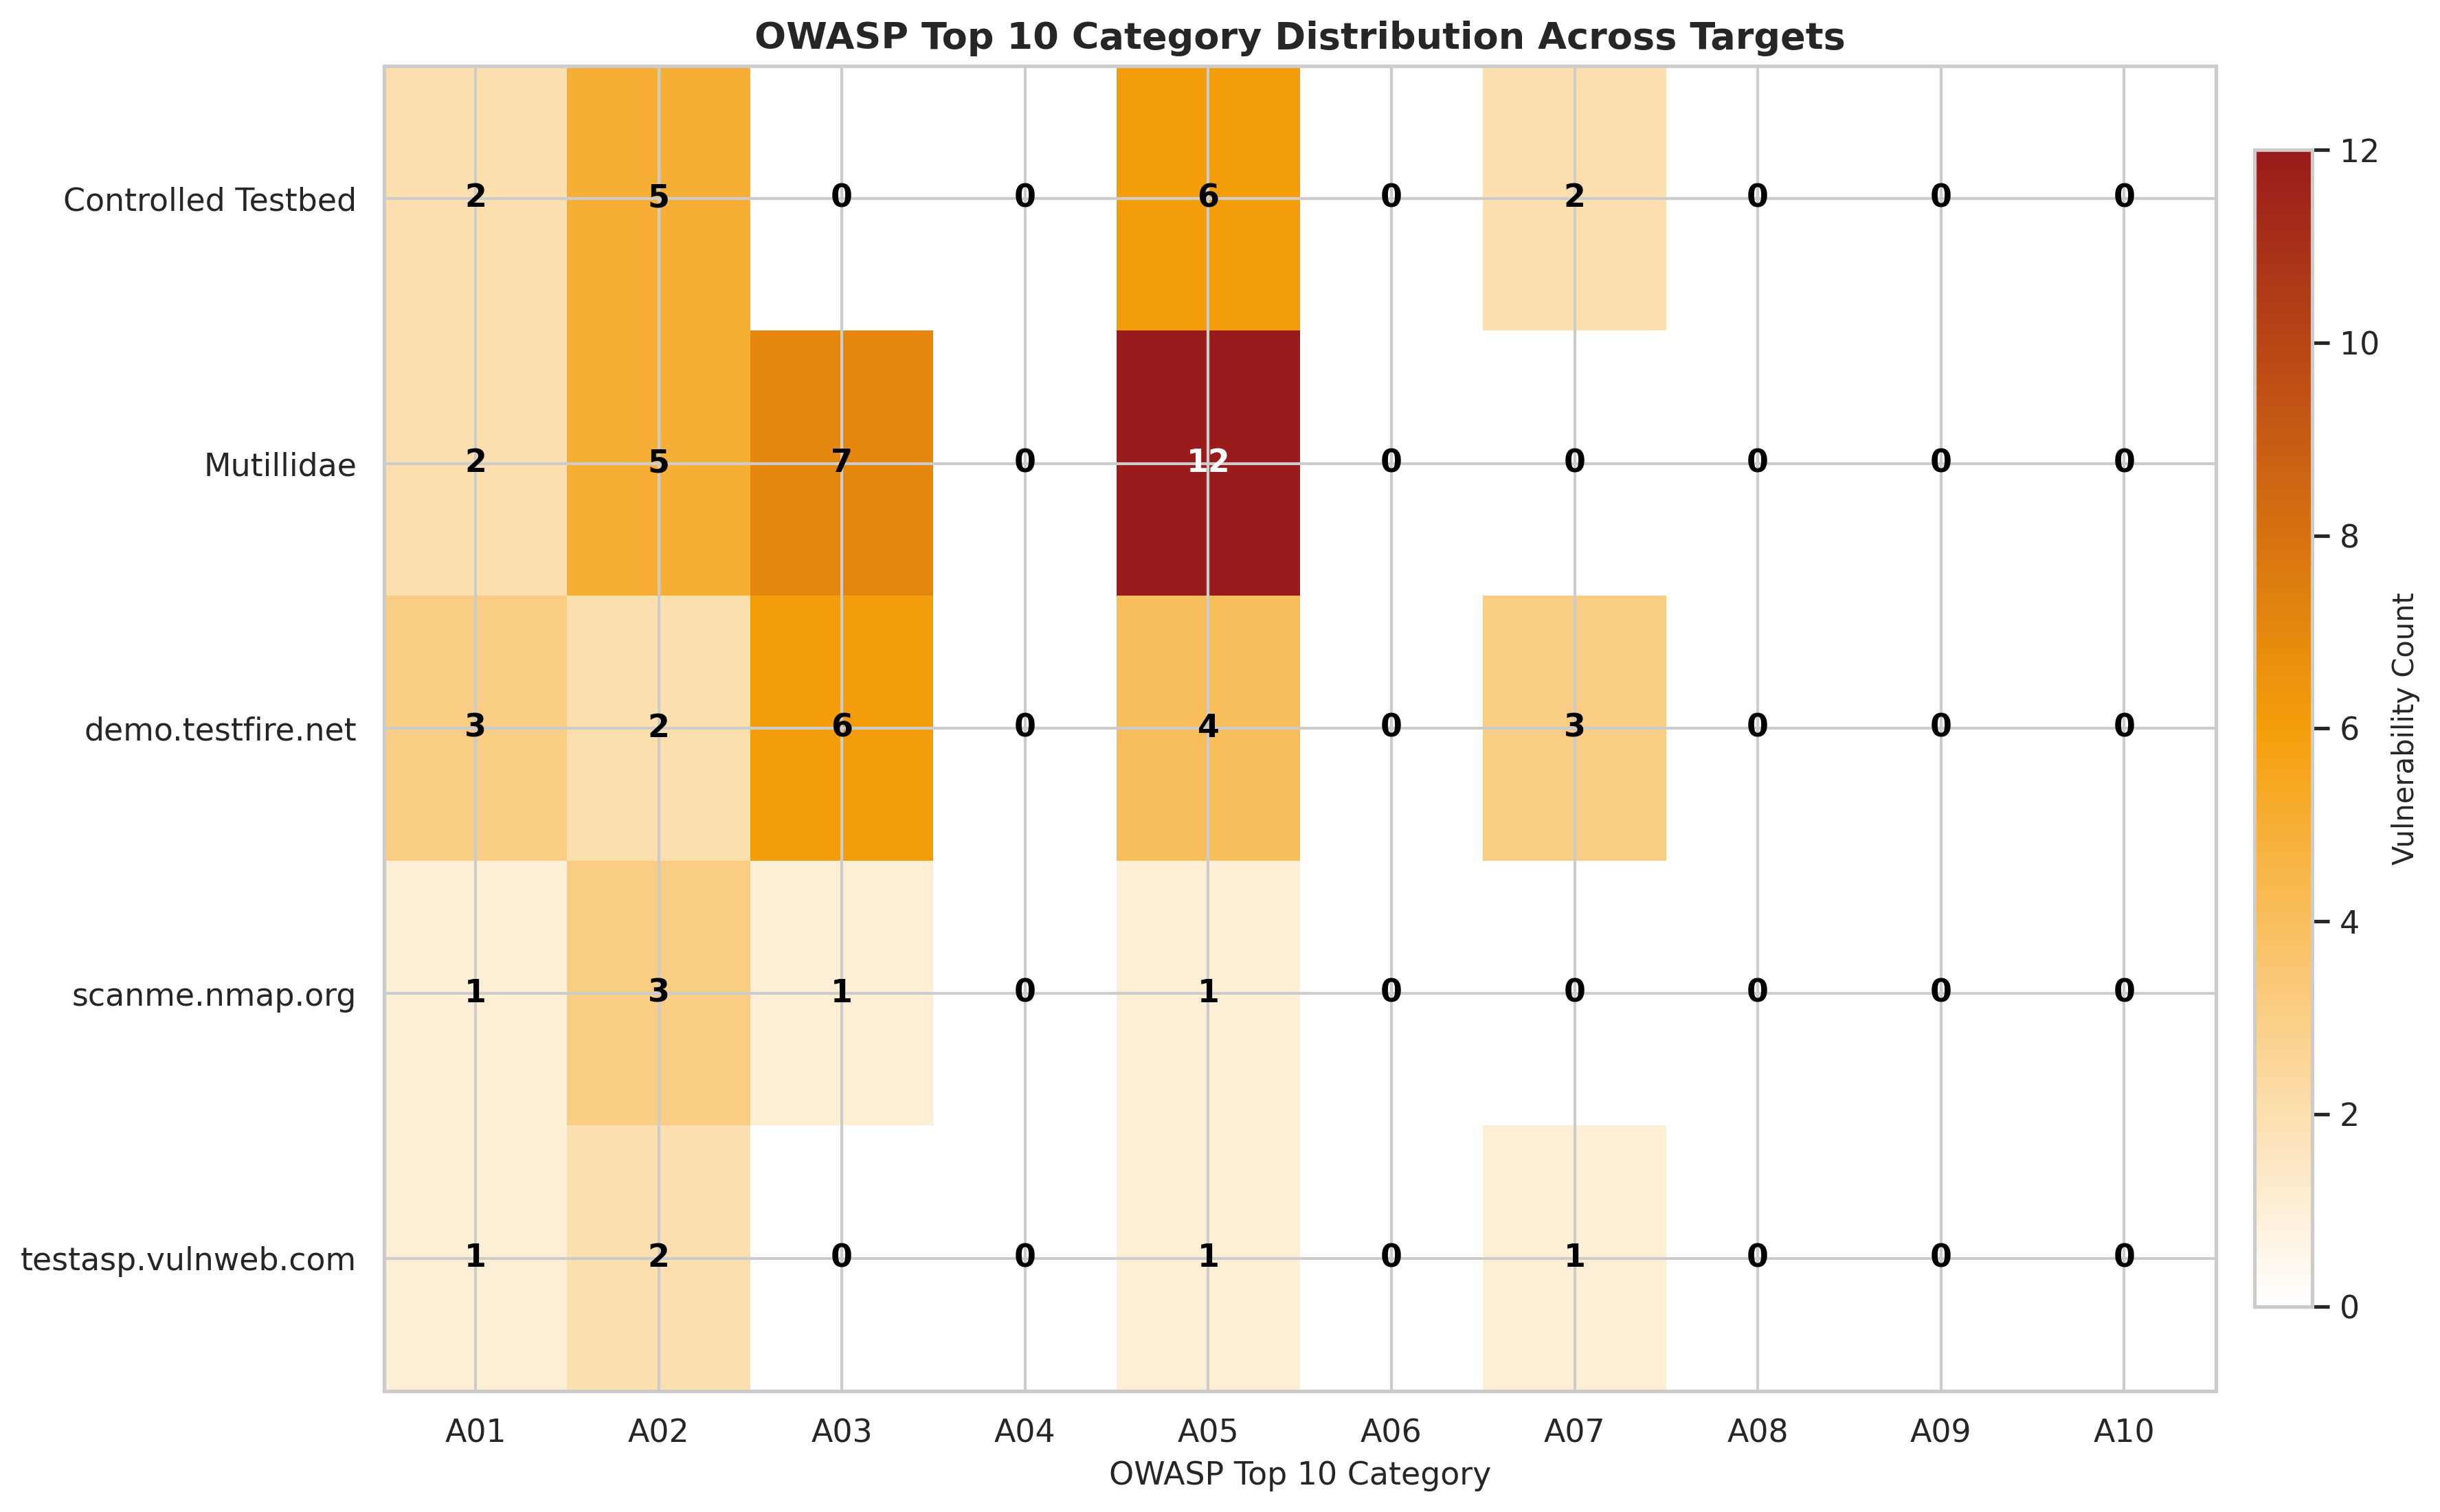
\includegraphics[width=\textwidth]{chapter4figures/fig_owasp_heatmap.png}
\caption{OWASP Top~10 category heatmap across all five baseline scans, with cell
  values indicating the number of vulnerabilities mapped to each category.}
\label{fig:owasp-heatmap}
\end{figure}

The baseline scans consistently detected vulnerabilities across four of the ten
OWASP Top~10 categories: A01 (Broken Access Control), A02 (Cryptographic Failures),
A03 (Injection) and A05 (Security Misconfiguration). The remaining six categories
received zero detections across four of the five targets. This pattern reflects a
structural constraint of the scanning layer rather than a deficiency in the
classification pipeline: the system operates at the network level via Nmap, and the
four detected categories align with what service enumeration, NSE scripting and
header analysis can observe. The exception is demo.testfire.net, which achieved 5/10
coverage by additionally triggering A07 (Identification and Authentication Failures)
detections, a result consistent with its financial-application design exposing
authentication endpoints that Nmap's NSE scripts can partially enumerate.
Categories such as A04 (Insecure Design), A08 (Software and Data Integrity Failures)
and A09 (Security Logging and Monitoring Failures) are architectural or operational
concerns that no automated network-layer scanner can detect. The 40\% OWASP coverage
figure across four of five targets should be read as the system reporting what it can
detect rather than inflating coverage beyond its scanner's reach.

% ─────────────────────────────────────────────
\section{Phase 2: Contextual Weighting Comparative Analysis}
\label{sec:phase2-results}

% Contextual weighting comparison table — Mutillidae only
\begin{table}[H]
\centering
\caption{Phase~2 contextual weighting comparison on the Mutillidae target.}
\label{tab:contextual-comparison}
\small
\renewcommand{\arraystretch}{1.45}
\setlength{\tabcolsep}{5pt}
\begin{tabularx}{\textwidth}{
  >{\raggedright\arraybackslash}p{4.5cm}
  >{\centering\arraybackslash}p{1.8cm}
  >{\centering\arraybackslash}p{1.8cm}
  >{\centering\arraybackslash}X}
\toprule
\rowcolor{headerblue}
\textcolor{headertext}{\textbf{Configuration}} &
\textcolor{headertext}{\textbf{Total Deductions}} &
\textcolor{headertext}{\textbf{Grade}} &
\textcolor{headertext}{\textbf{Notes}} \\
\midrule
\rowcolor{rowlight}
\texttt{contextualWeighting} OFF (flat) & 107 & F & Flat severity scoring only \\
\rowcolor{rowwhite}
All toggles ON (contextual)             & 181 & F & Contextual multipliers active \\
\midrule
\rowcolor{rowlight}
\textbf{Amplification} & \multicolumn{3}{l}{$(181 - 107) \div 107 = +69.2\%$} \\
\bottomrule
\end{tabularx}
\renewcommand{\arraystretch}{1.0}
\end{table}

Contextual weighting produced a 69.2\% amplification in total severity deductions on the Mutillidae baseline, raising the score from 107 (flat) to 181 (contextual), as shown in Table~\ref{tab:contextual-comparison} and Figure~\ref{fig:contextual-comparison}. Port exposure on web-facing services is the dominant contextual factor: the \texttt{contextualWeighting} module identified Mutillidae's HTTP and HTTPS endpoints as high-exposure services warranting a 1.5$\times$ multiplier; Figure~\ref{fig:multiplier-heatmap} confirms that the service exposure and authentication weakness channels both remained at 1.0$\times$ throughout, meaning those two multiplier dimensions had no measurable effect on this target.

The combined 1.5$\times$ multiplier applied to approximately 60\% of the vulnerability set accounts for the bulk of the 74-point differential, confirming that the weighting system meaningfully differentiates risk profiles beyond flat CVSS-style severity assignment; the inactive channels limit conclusions about the full multiplier model from this target alone.

\begin{figure}[H]
\centering
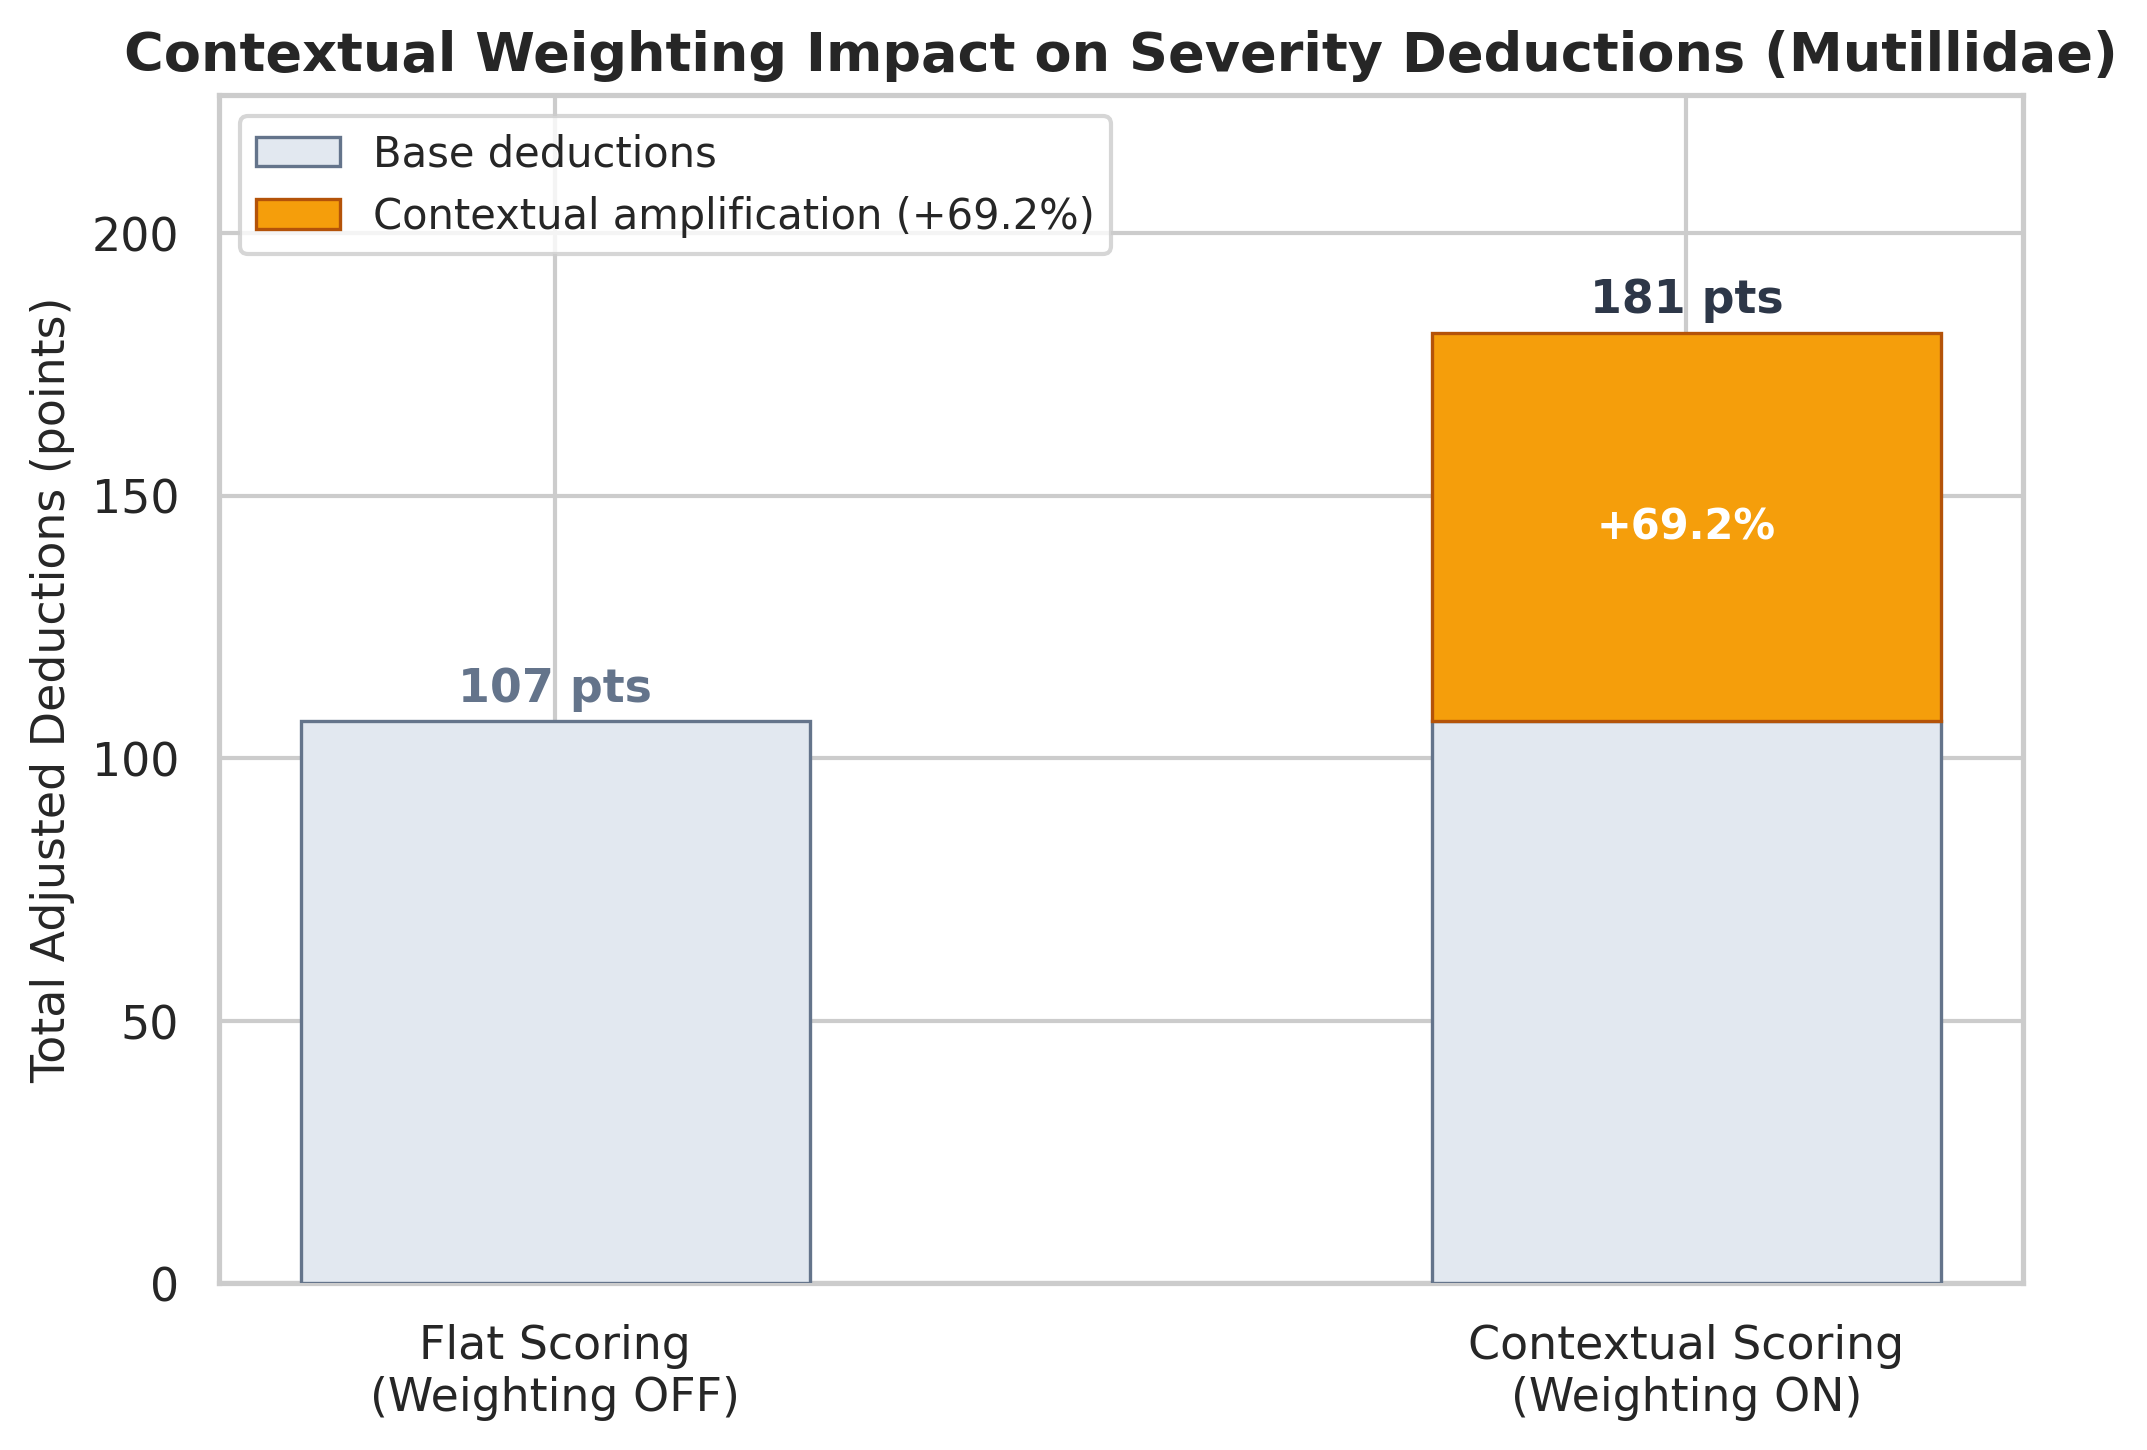
\includegraphics[width=\textwidth]{chapter4figures/fig_contextual_comparison.png}
\caption{Comparison of flat (weighting OFF) versus contextual (weighting ON) severity
  deductions on the Mutillidae target, showing the 69.2\% amplification produced by
  the contextual multiplier system.}
\label{fig:contextual-comparison}
\end{figure}

\begin{figure}[H]
\centering
\includegraphics[width=1.1\textwidth]{chapter4figures/fig_multiplier_heatmap only.png}
\caption{Per-vulnerability contextual multiplier values for the Mutillidae baseline scan,
  showing port exposure, service exposure, authentication weakness and combined
  multiplier across all 26 findings.}
\label{fig:multiplier-heatmap}
\end{figure}

\begin{figure}[H]
\centering
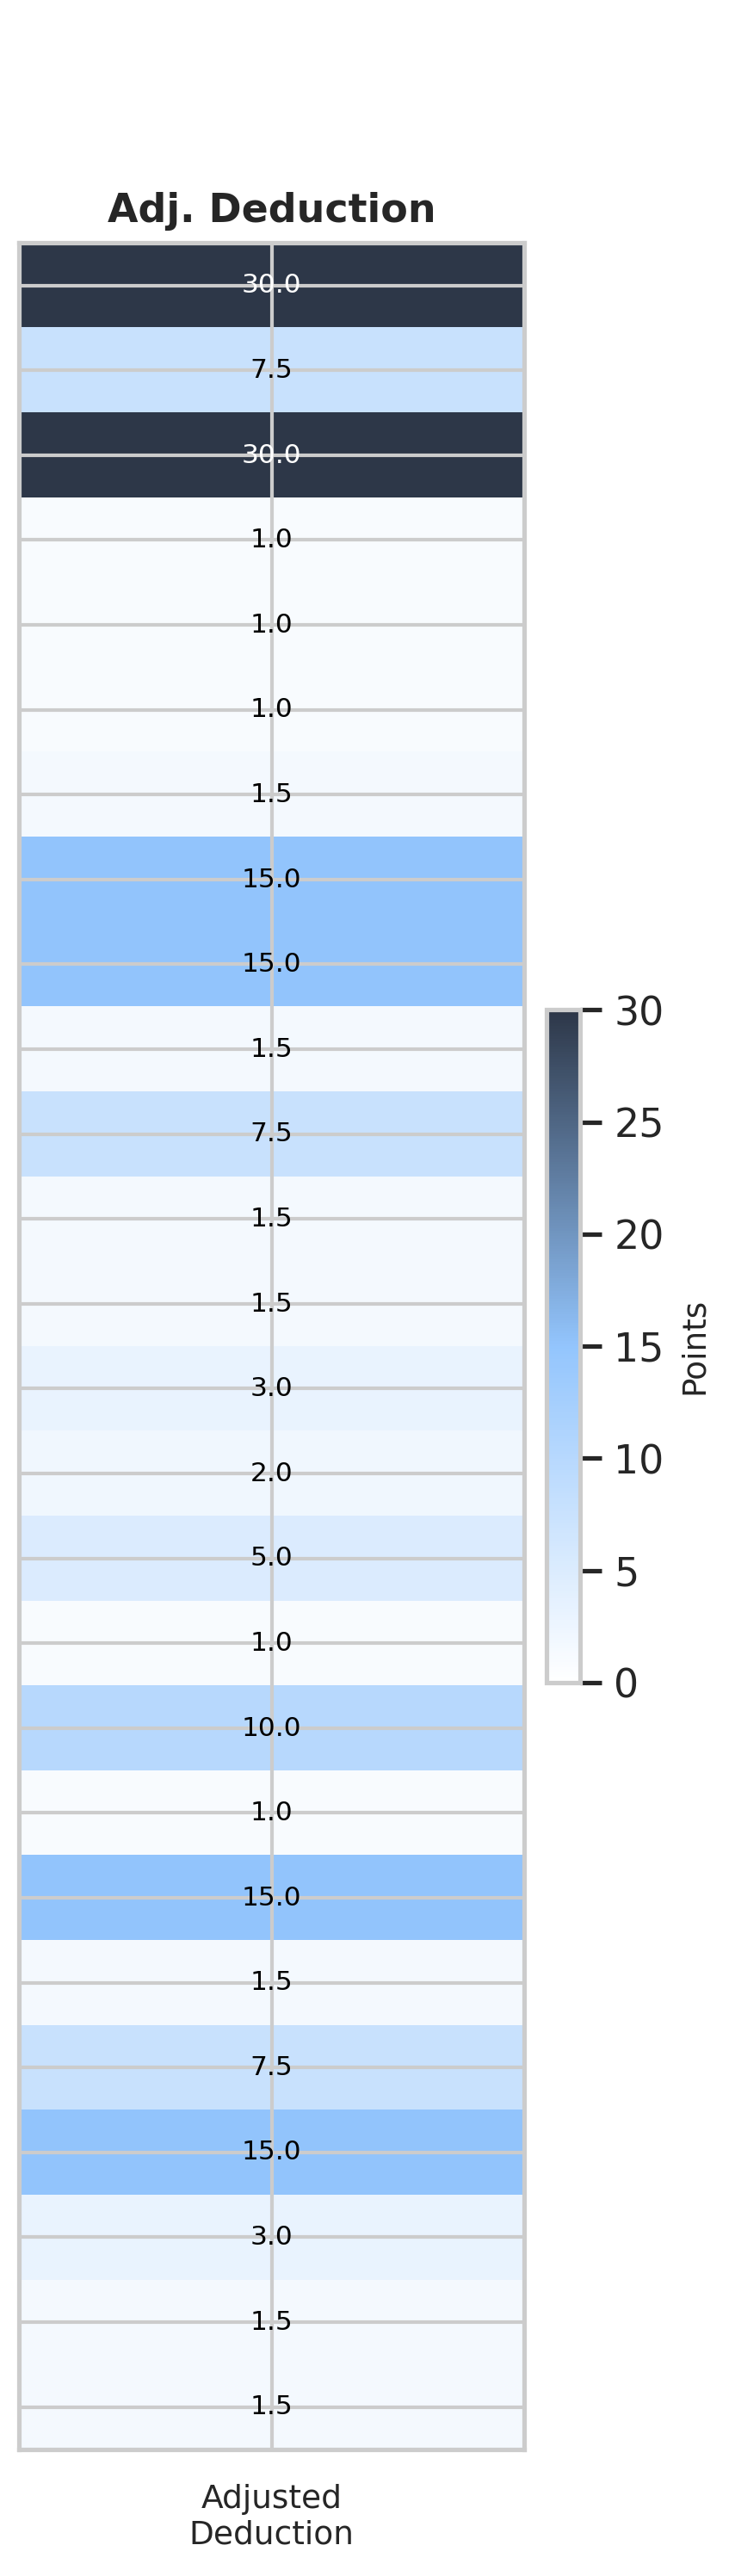
\includegraphics[height=0.82\textheight,keepaspectratio]{chapter4figures/fig_multiplier_heatmap - Copy (2).png}
\caption{Adjusted deduction scores for each vulnerability in the Mutillidae
  baseline scan, corresponding to the multiplier values in Figure~\ref{fig:multiplier-heatmap}.}
\label{fig:adj-deduction}
\end{figure}

% ─────────────────────────────────────────────
\section{Phase 3: Ablation Testing}
\label{sec:phase3-results}

% Ablation results table — Mutillidae target, one toggle off per row
\begin{table}[H]
\centering
\caption{Phase~3 ablation test results on the Mutillidae target. Each row disables a single pipeline component while all others remain active.}
\label{tab:ablation-results}
\small
\renewcommand{\arraystretch}{1.45}
\setlength{\tabcolsep}{5pt}
\begin{tabularx}{\textwidth}{
  >{\raggedright\arraybackslash}p{4.0cm}
  >{\centering\arraybackslash}p{1.5cm}
  >{\centering\arraybackslash}p{1.5cm}
  >{\raggedright\arraybackslash}X}
\toprule
\rowcolor{headerblue}
\textcolor{headertext}{\textbf{Configuration}} &
\textcolor{headertext}{\textbf{Sev. Ded.}} &
\textcolor{headertext}{\textbf{$\Delta$ vs Full}} &
\textcolor{headertext}{\textbf{Observed Effect}} \\
\midrule
\rowcolor{rowlight}
Full pipeline (baseline)              & 181 & ---   & All components active \\
\rowcolor{rowwhite}
\texttt{contextualWeighting} OFF      & 107 & $-74$ & Port exposure multipliers removed \\
\rowcolor{rowlight}
\texttt{owaspMapping} OFF             & 166 & $-15$ & All vulns collapse to A05 fallback \\
\rowcolor{rowwhite}
\texttt{aiAnalysis} OFF               & 181 & $0$   & Remediation quality removed, score unchanged \\
\rowcolor{rowlight}
\texttt{hallucinationGuard} OFF       & 165 & $-16$ & Validation layer removed \\
\bottomrule
\end{tabularx}
\renewcommand{\arraystretch}{1.0}
\end{table}

Disabling \texttt{contextualWeighting} produced the largest single-component delta at $-74$ points (181 to 107), confirming contextual weighting as the highest-impact component and showing the contextual layer accounts for approximately 41\% of total severity deductions in the full configuration. The design as a distinct, toggleable module means operators who prefer flat scoring can disable the multiplier system without affecting the remainder of the pipeline.

Disabling \texttt{owaspMapping} reduced deductions by 15 points as all vulnerabilities collapsed to the A05 fallback, eliminating the category breadth penalty the scoring engine applies when findings span multiple OWASP categories. The modest reduction confirms the breadth penalty contributes a secondary but measurable effect, and that the fallback assigns a conservative default rather than discarding unmapped findings.

Disabling \texttt{aiAnalysis} produced a zero-point delta, as the AI component contributes remediation depth rather than numerical scoring; the $+10$ bonus affects grade interpretation rather than the severity deduction total. Disabling \texttt{hallucinationGuard} reduced deductions by 16 points, a contribution comparable to the OWASP breadth penalty and consistent with the guard's role as a validation layer applying confidence-weighted adjustments to AI classifications rather than functioning as a primary scoring mechanism.

\begin{figure}[H]
\centering
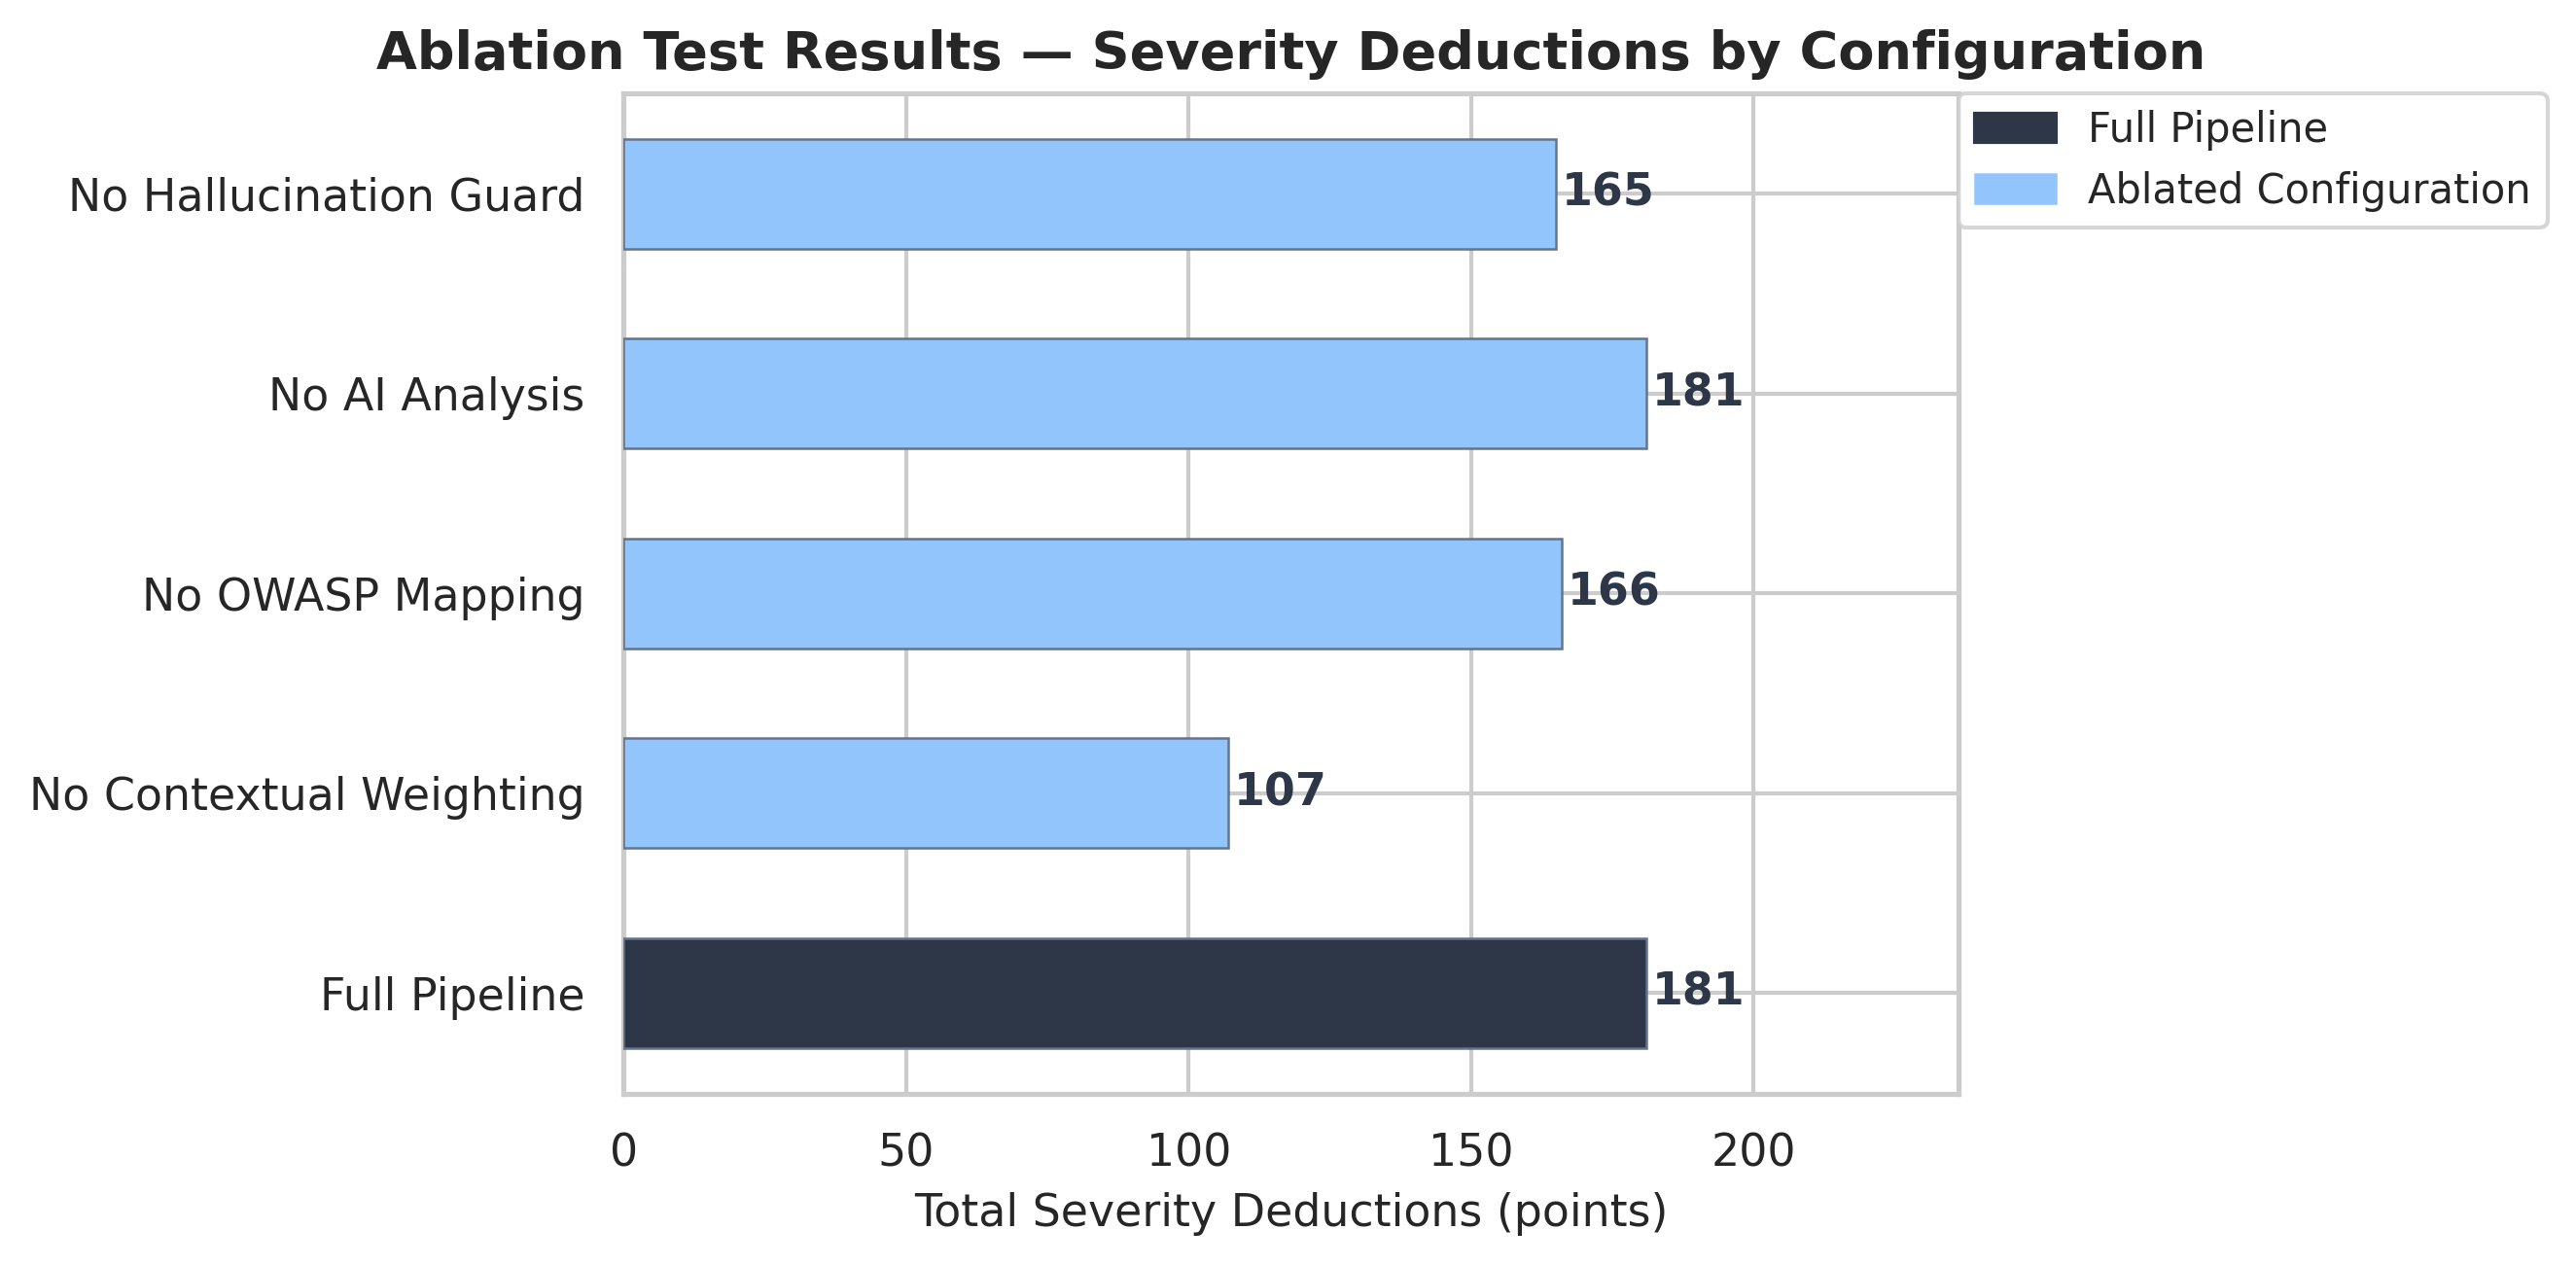
\includegraphics[width=\textwidth]{chapter4figures/fig_ablation_scores.png}
\caption{Ablation test severity deductions on the Mutillidae target, comparing the
  full pipeline against each single-component removal configuration.}
\label{fig:ablation-scores}
\end{figure}

% ─────────────────────────────────────────────
\section{Phase 4: Lifecycle Delta Demonstration}
\label{sec:phase4-results}

Phase~4 was conducted exclusively on the controlled testbed
(\texttt{127.0.0.1:8080}), which is the only target whose vulnerability
configuration permits selective remediation between scan cycles. The baseline
scan was followed by targeted remediation of eight vulnerabilities, after which
a rescan was performed and the delta comparison module generated the results
presented in Table~\ref{tab:delta-comparison}.

\begin{table}[H]
\centering
\caption{Phase~4 lifecycle delta comparison on the controlled testbed, showing
  before (baseline) and after (remediated) scan results.}
\label{tab:delta-comparison}
\small
\renewcommand{\arraystretch}{1.45}
\setlength{\tabcolsep}{4pt}
\begin{tabularx}{\textwidth}{
  >{\raggedright\arraybackslash}X
  >{\centering\arraybackslash}p{1.35cm}
  >{\centering\arraybackslash}p{1.55cm}
  >{\centering\arraybackslash}p{1.45cm}
  >{\centering\arraybackslash}p{1.00cm}
  >{\centering\arraybackslash}p{1.00cm}
  >{\centering\arraybackslash}p{0.80cm}}
\toprule
\rowcolor{headerblue}
\textcolor{headertext}{\textbf{Scan}} &
\textcolor{headertext}{\textbf{Score}} &
\textcolor{headertext}{\textbf{Total Vulns}} &
\textcolor{headertext}{\textbf{Critical}} &
\textcolor{headertext}{\textbf{High}} &
\textcolor{headertext}{\textbf{Med.}} &
\textcolor{headertext}{\textbf{Low}} \\
\midrule
\rowcolor{rowlight}
Before (Baseline)   & 3  & 15 & 0 & 2 & 3 & 2 \\
\rowcolor{rowwhite}
After (Remediated)  & 60 & 7  & 0 & 1 & 1 & 1 \\
\midrule
\rowcolor{rowlight}
\textbf{Delta}      & \textbf{+57} & \textbf{$-8$} & \textbf{0} & \textbf{$-1$} & \textbf{$-2$} & \textbf{$-1$} \\
\bottomrule
\end{tabularx}
\renewcommand{\arraystretch}{1.0}
\end{table}

The score improved by 57 points, from 3 to 60, following remediation of 8 of 15 vulnerabilities, representing a 53\% reduction in total findings as shown in Figure~\ref{fig:delta-comparison}. The post-remediation scan correctly identified all 7 remaining findings as persisting vulnerabilities not targeted in this cycle, demonstrating that the delta comparison module accurately distinguishes resolved from persisting findings. The residual 1 High and 1 Medium findings held the post-remediation score at 60, confirming that persisting high-severity vulnerabilities are penalised proportionally as designed.

\begin{figure}[H]
\centering
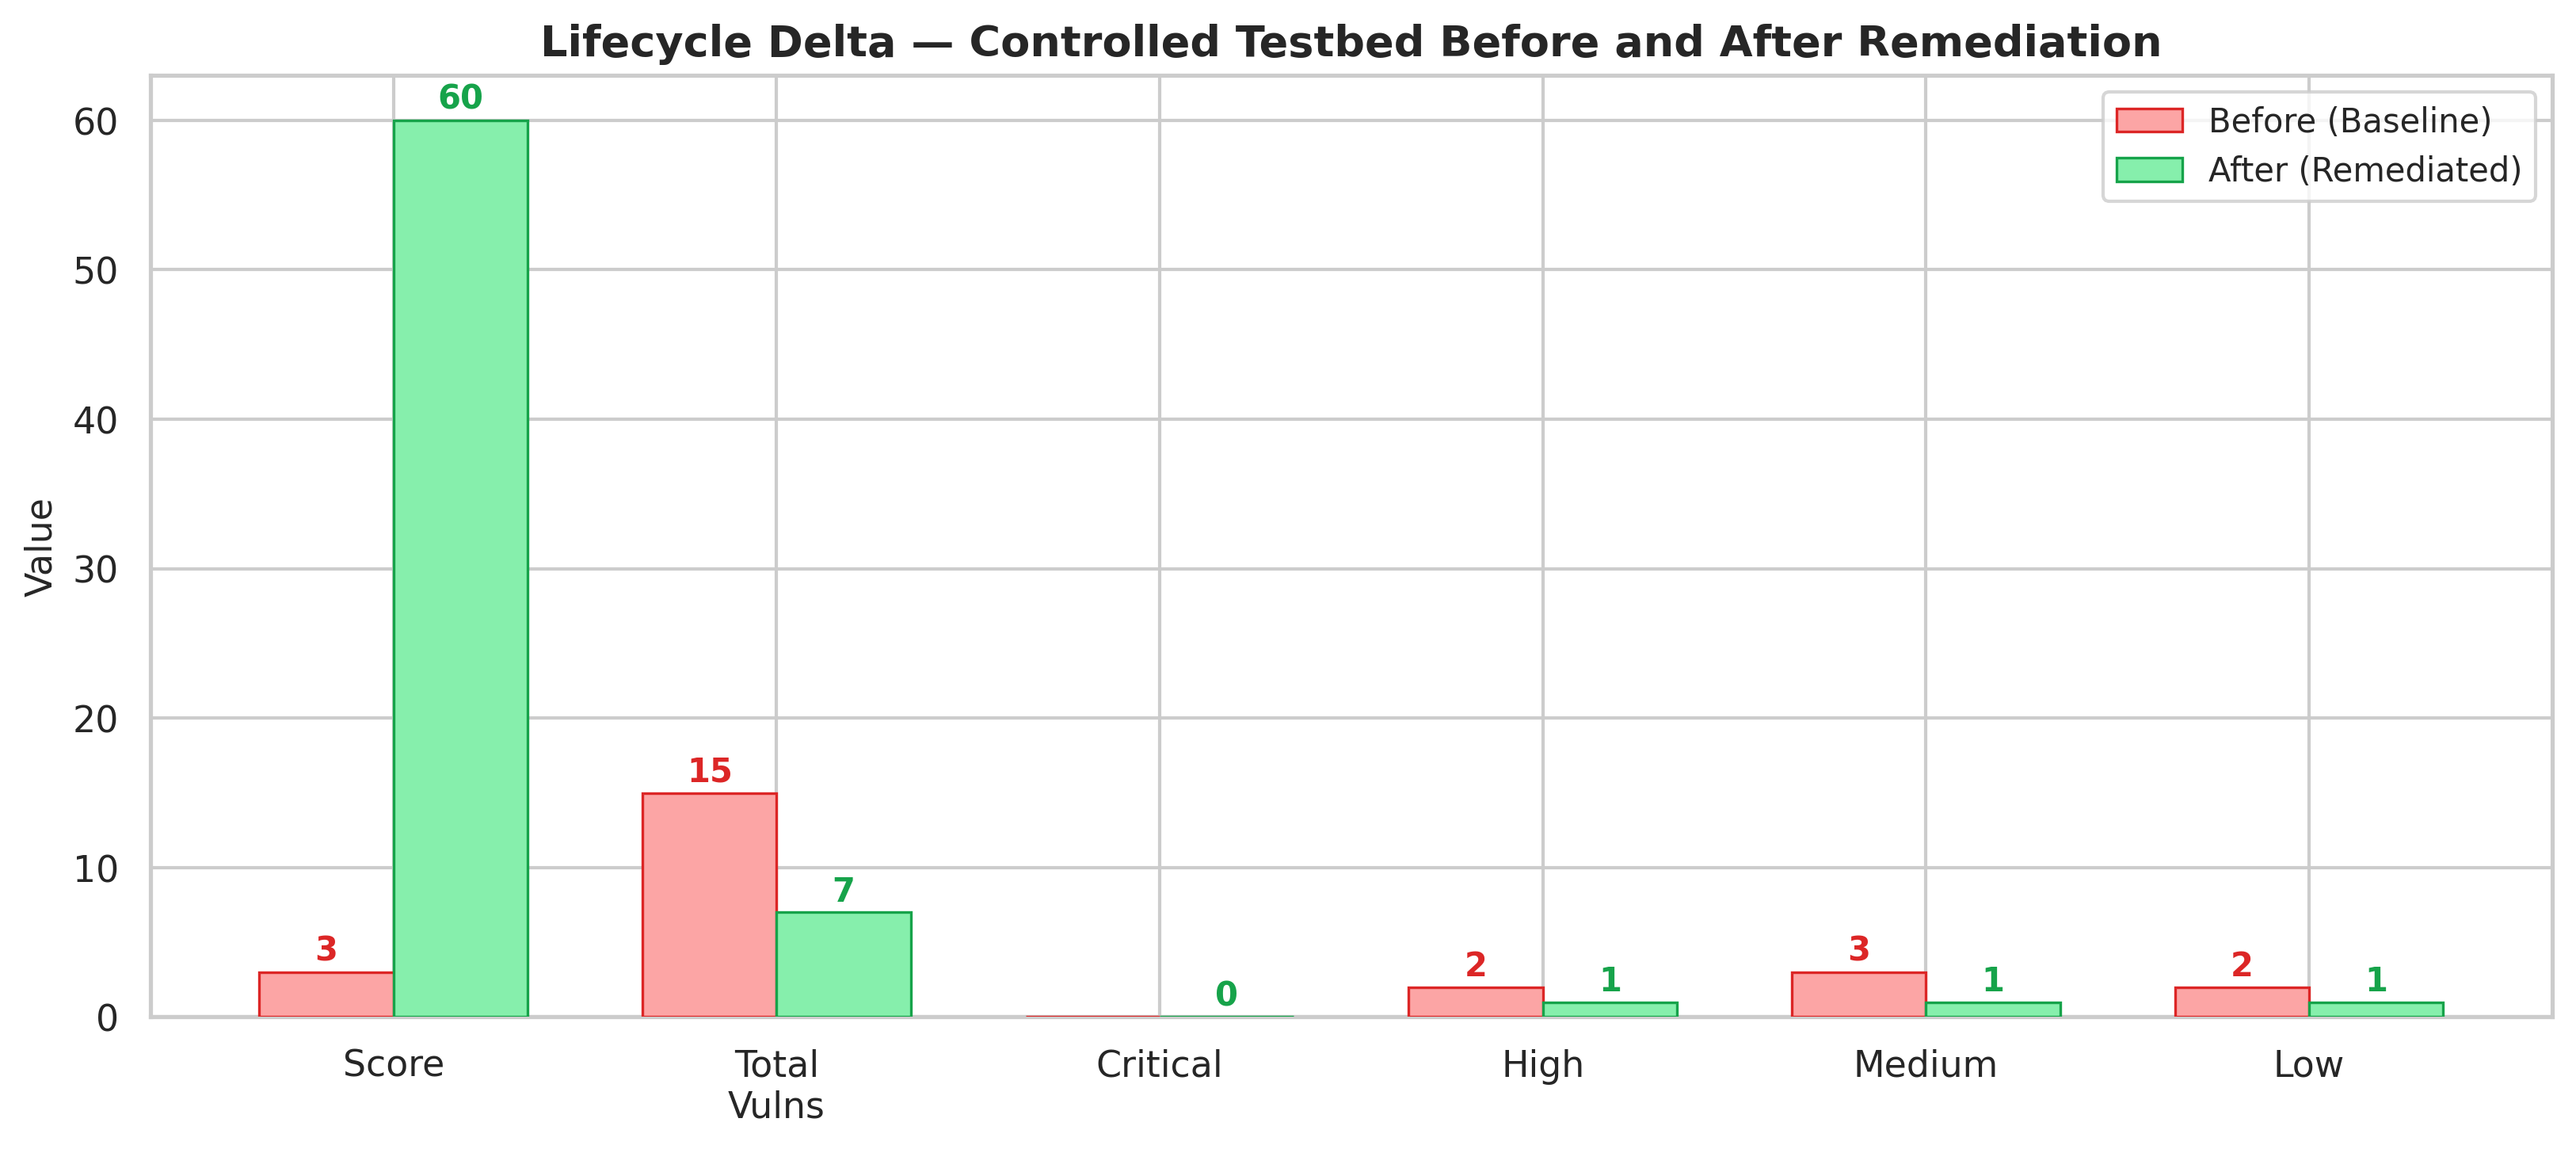
\includegraphics[width=\textwidth]{chapter4figures/fig_delta_comparison.png}
\caption{Lifecycle delta comparison between the baseline and remediated scans on
  the controlled testbed, showing the score improvement from 3 to 60 and the
  reduction from 15 to 7 total vulnerabilities.}
\label{fig:delta-comparison}
\end{figure}

% ─────────────────────────────────────────────
\section{Phase 5: Longitudinal Hallucination Reliability}
\label{sec:phase5-results}

% Hallucination metrics table — one row per scan across all targets
\begin{table}[H]
\centering
\caption{Longitudinal hallucination guard metrics across all evaluation scans
  where both \texttt{aiAnalysis} and \texttt{hallucinationGuard} were enabled.}
\label{tab:hallucination-longitudinal}
\footnotesize
\renewcommand{\arraystretch}{1.45}
\setlength{\tabcolsep}{4pt}
\begin{tabularx}{\textwidth}{
  >{\centering\arraybackslash}p{0.6cm}
  >{\raggedright\arraybackslash}p{4.6cm}
  >{\centering\arraybackslash}p{1.4cm}
  >{\centering\arraybackslash}p{1.3cm}
  >{\raggedright\arraybackslash}X}
\toprule
\rowcolor{headerblue}
\textcolor{headertext}{\textbf{Scan}} &
\textcolor{headertext}{\textbf{Target / Configuration}} &
\textcolor{headertext}{\textbf{Trust Score}} &
\textcolor{headertext}{\textbf{Fab.\ CVEs}} &
\textcolor{headertext}{\textbf{Notes}} \\
\midrule
\rowcolor{rowlight}
1  & Mutillidae (baseline)                    & $\sim$55 & 0 & Below threshold \\
\rowcolor{rowwhite}
2  & Mutillidae (No OWASP)                    & 0        & 0 & Guard detects total OWASP disagreement \\
\rowcolor{rowlight}
3  & Controlled Testbed (baseline)            & $\sim$50 & 0 & Below threshold \\
\rowcolor{rowwhite}
4  & Controlled Testbed (Phase~2)             & $\sim$47 & 0 & Below threshold \\
\rowcolor{rowlight}
5  & Controlled Testbed (No OWASP)            & $\sim$40 & 0 & Below threshold \\
\rowcolor{rowwhite}
6  & scanme.nmap.org (baseline)               & $\sim$72 & 0 & Above threshold \\
\rowcolor{rowlight}
7  & scanme.nmap.org (Phase~2)                & $\sim$71 & 0 & Above threshold \\
\rowcolor{rowwhite}
8  & testasp.vulnweb.com (baseline)           & $\sim$85 & 0 & Above threshold \\
\rowcolor{rowlight}
9  & testasp.vulnweb.com (Phase~2)            & $\sim$85 & 0 & Above threshold \\
\rowcolor{rowwhite}
10 & demo.testfire.net (baseline)             & $\sim$38 & 0 & Below threshold \\
\rowcolor{rowlight}
11 & demo.testfire.net (Phase~2)              & $\sim$38 & 0 & Below threshold \\
\bottomrule
\end{tabularx}
\renewcommand{\arraystretch}{1.0}
\end{table}

Zero fabricated CVEs were recorded across all 11 scans in Table~\ref{tab:hallucination-longitudinal}, confirming that the AI model produced no invented vulnerability identifiers in any tested configuration. Trust scores varied from 0 on the Mutillidae ``No OWASP'' configuration (expected: with the mapper disabled, the guard correctly detects near-total OWASP disagreement) to approximately 85 on testasp.vulnweb.com; only scanme.nmap.org and testasp.vulnweb.com consistently exceeded the 70-point threshold, as shown in Figure~\ref{fig:trust-scores}. Figure~\ref{fig:hallucination-breakdown} shows Mutillidae accumulating the highest risk flag count at approximately 18, consistent with its larger vulnerability set producing more opportunities for AI classification disagreements.

\begin{figure}[H]
\centering
\makebox[\textwidth][c]{%
  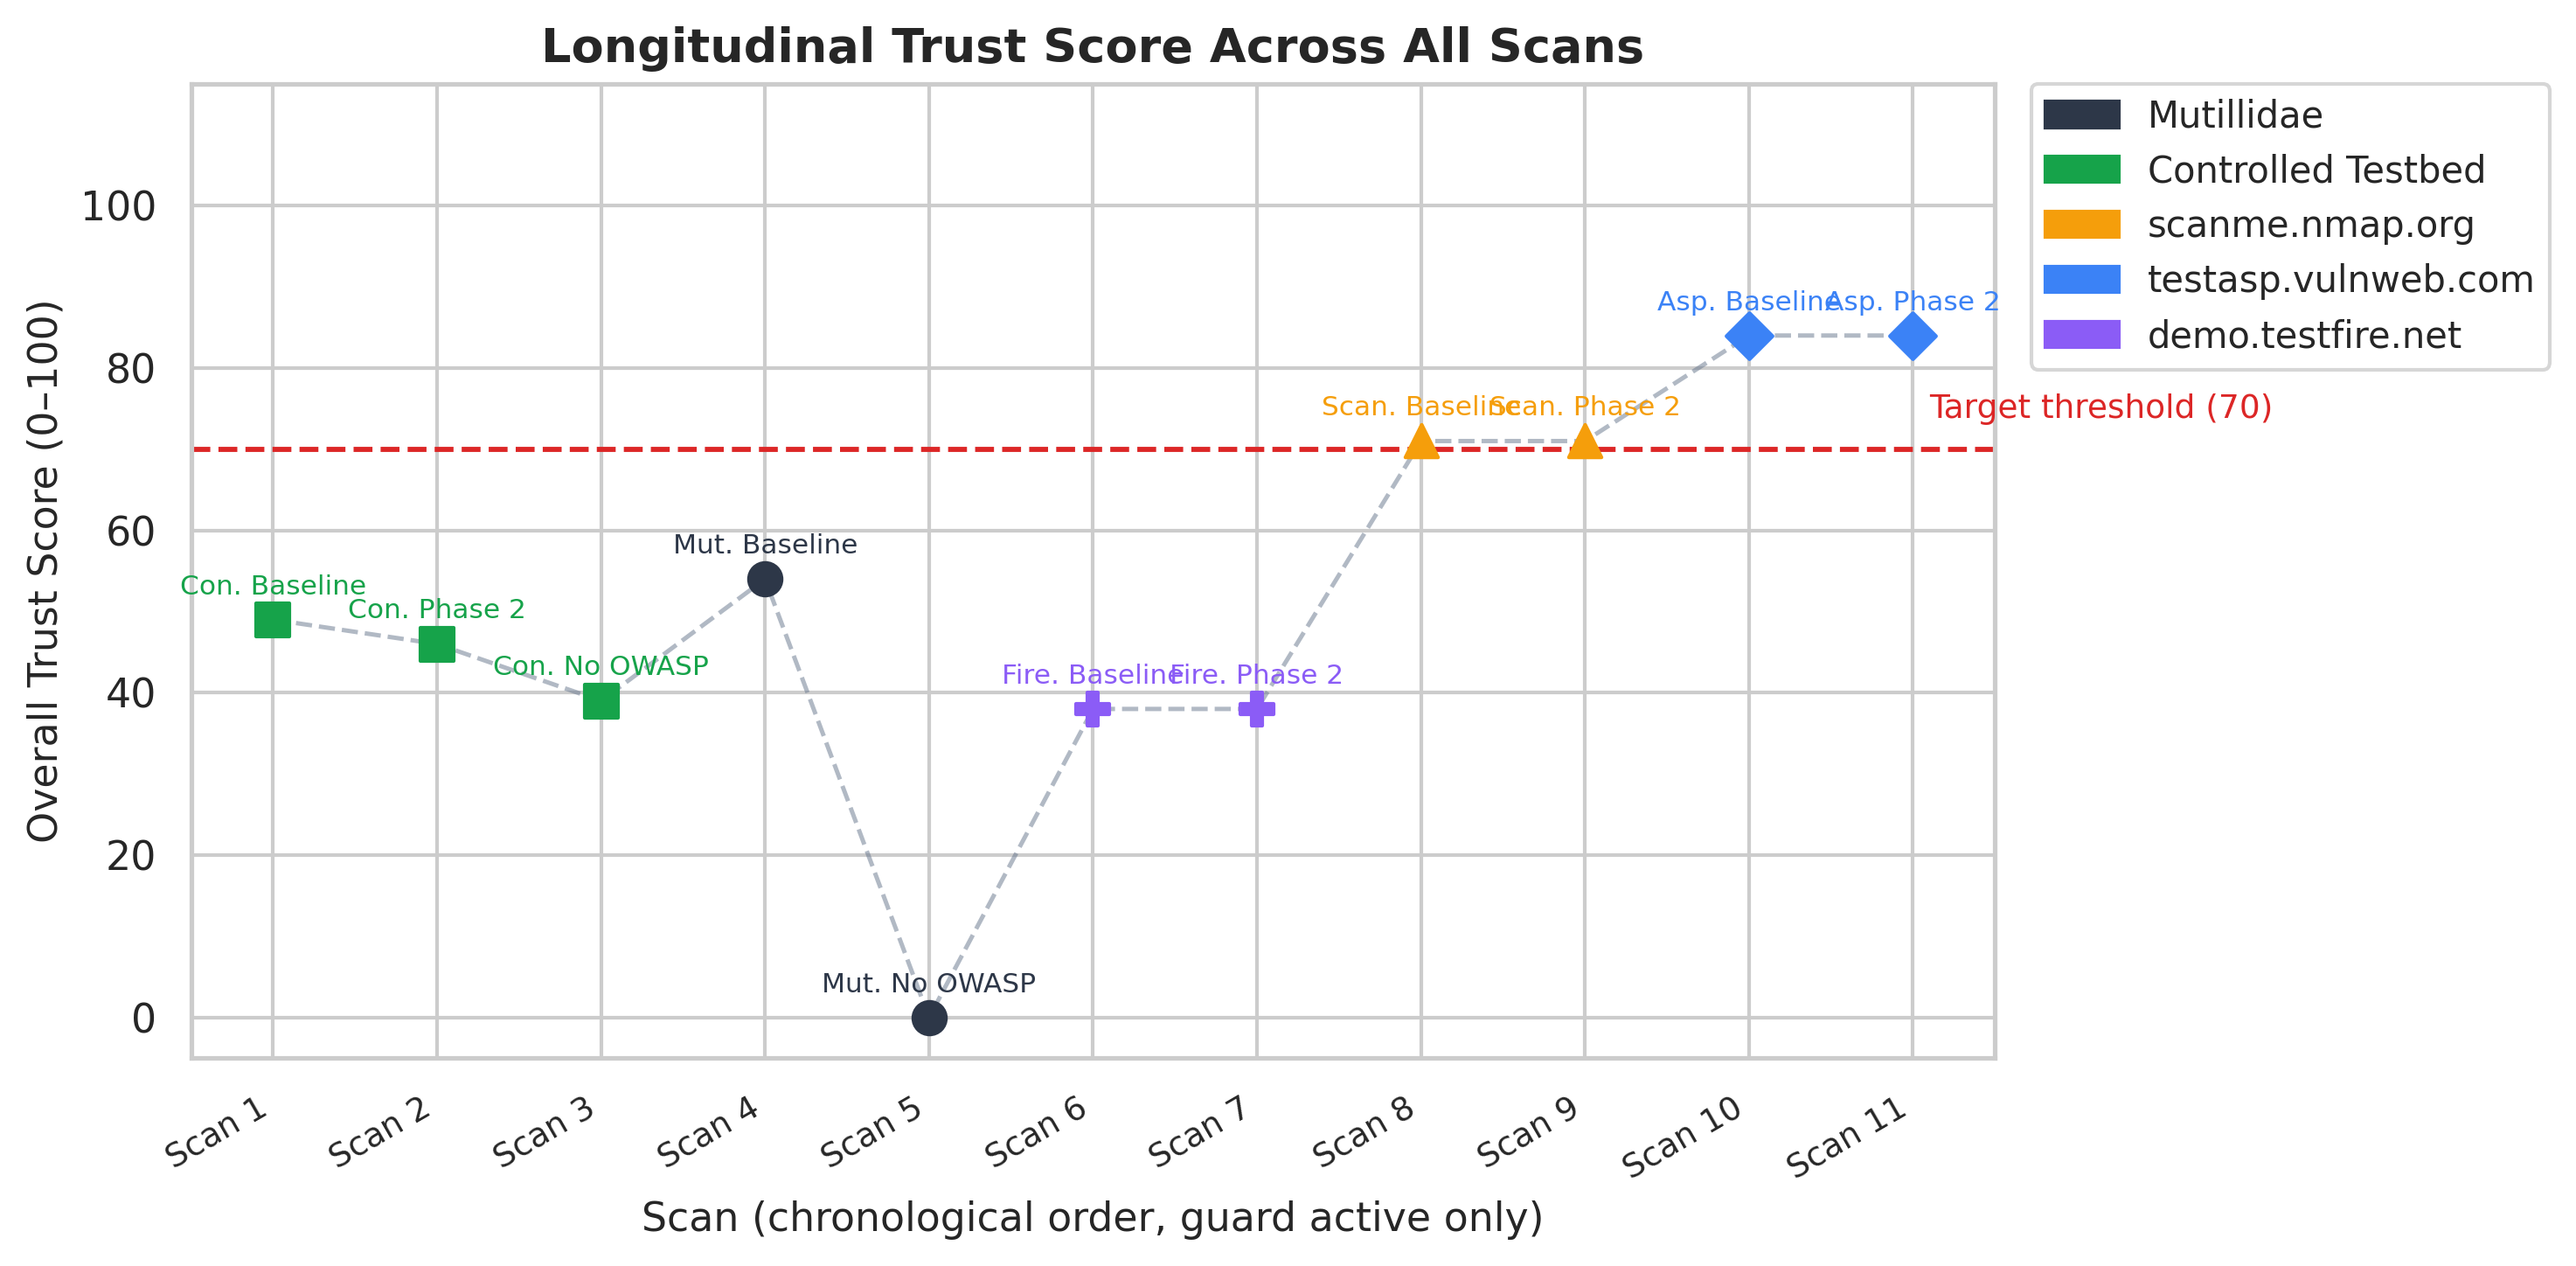
\includegraphics[width=1.15\textwidth]{chapter4figures/fig_trust_scores.png}%
}
\caption{Trust scores across all evaluation scans, with the 70-point threshold
  indicated. Only \mbox{scanme.nmap.org} and \mbox{testasp.vulnweb.com}
  consistently exceed the threshold.}
\label{fig:trust-scores}
\end{figure}

\begin{figure}[H]
\centering
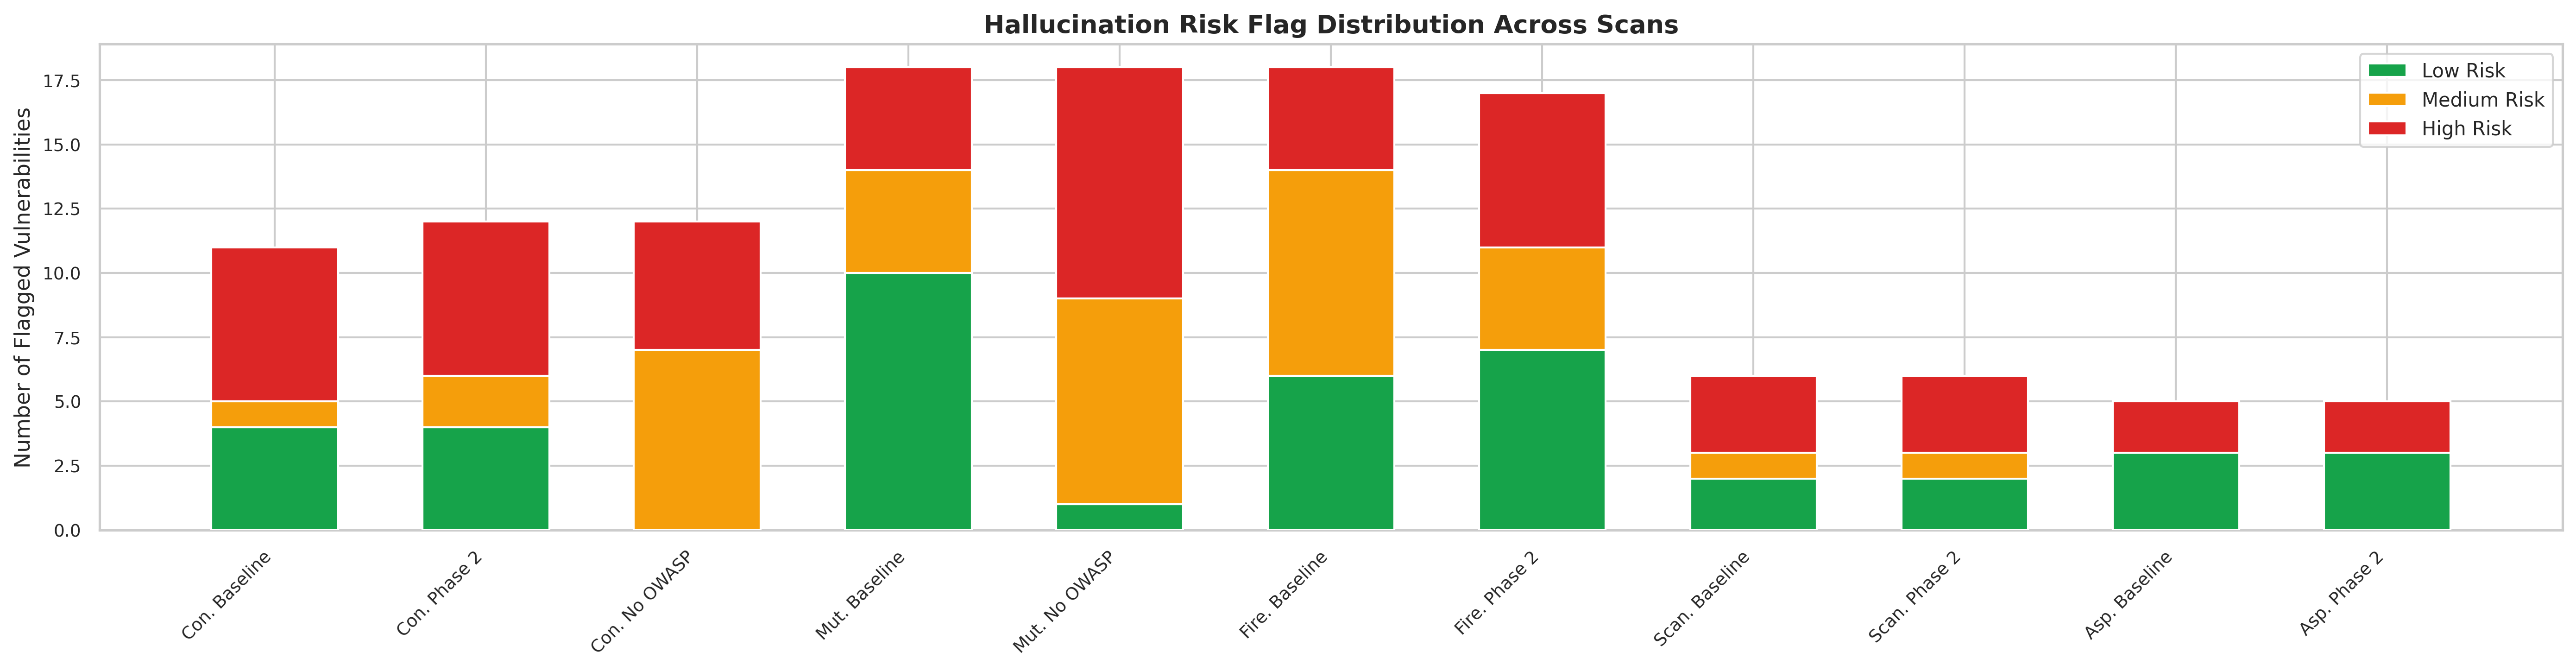
\includegraphics[width=\textwidth]{chapter4figures/fig_hallucination_breakdown.png}
\caption{Hallucination risk flag breakdown per scan, showing stacked Low, Medium
  and High risk flags. Mutillidae baseline exhibits the highest total flag count
  at approximately 18 flags.}
\label{fig:hallucination-breakdown}
\end{figure}

The 70-point target was not met on three of the five evaluation targets, an outcome that reflects genuine AI classification inconsistencies rather than a systematic deficiency in the guard itself. The consistently low scores on demo.testfire.net (approximately 38) indicate higher disagreement rates on the IIS/ASP.NET stack; the variation across targets confirms that trust score is sensitive to target complexity and technology stack, and that the threshold may require calibration for non-PHP environments. Only the port exposure multiplier channel activated across all five targets, with service exposure and authentication weakness channels remaining at 1.0$\times$ throughout.

% ─────────────────────────────────────────────
\section{Tool Capability Comparison}
\label{sec:tool-comparison}

Table~\ref{tab:tool-comparison} positions PurpleTeam Suite against six representative tools, measuring integration completeness across the full assessment lifecycle rather than raw detection performance.

\begin{table}[H]
\centering
\caption{Feature comparison across representative vulnerability assessment tools. Integration completeness is assessed rather than raw detection performance.}
\label{tab:tool-comparison}
\footnotesize
\renewcommand{\arraystretch}{1.45}
\setlength{\tabcolsep}{2pt}
\begin{tabularx}{\textwidth}{
  >{\raggedright\arraybackslash}X
  >{\centering\arraybackslash}p{1.10cm}
  >{\centering\arraybackslash}p{1.10cm}
  >{\centering\arraybackslash}p{1.10cm}
  >{\centering\arraybackslash}p{1.10cm}
  >{\centering\arraybackslash}p{1.10cm}
  >{\centering\arraybackslash}p{1.10cm}
  >{\centering\arraybackslash}p{1.10cm}}
\toprule
\rowcolor{headerblue}
\textcolor{headertext}{\textbf{Capability}} &
\makecell{\rotatebox{90}{\textcolor{headertext}{\textbf{PurpleTeam}}}} &
\makecell{\rotatebox{90}{\textcolor{headertext}{\textbf{Nmap}}}} &
\makecell{\rotatebox{90}{\textcolor{headertext}{\textbf{OWASP ZAP}}}} &
\makecell{\rotatebox{90}{\textcolor{headertext}{\textbf{OpenVAS}}}} &
\makecell{\rotatebox{90}{\textcolor{headertext}{\textbf{Burp Suite}}}} &
\makecell{\rotatebox{90}{\textcolor{headertext}{\textbf{Nessus}}}} &
\makecell{\rotatebox{90}{\textcolor{headertext}{\textbf{Splunk SOAR}}}} \\
\midrule
\rowcolor{rowlight}
OWASP Top~10 classification   & \checkmark & \ding{55} & \checkmark & Partial & \checkmark & Partial & Partial \\
\rowcolor{rowwhite}
Deterministic risk scoring     & \checkmark & \ding{55} & \checkmark & \checkmark & \checkmark & \checkmark & \checkmark \\
\rowcolor{rowlight}
Contextual weighting           & \checkmark & \ding{55} & \ding{55} & \ding{55} & \ding{55} & \ding{55} & Partial \\
\rowcolor{rowwhite}
AI remediation guidance        & \checkmark & \ding{55} & \ding{55} & \ding{55} & Partial & Partial & \checkmark \\
\rowcolor{rowlight}
Hallucination guard            & \checkmark & \ding{55} & \ding{55} & \ding{55} & \ding{55} & \ding{55} & \ding{55} \\
\rowcolor{rowwhite}
Iterative delta comparison     & \checkmark & \ding{55} & \ding{55} & Partial & \ding{55} & Partial & \checkmark \\
\rowcolor{rowlight}
Exportable PDF reporting       & \checkmark & Partial & \checkmark & \checkmark & \checkmark & \checkmark & \checkmark \\
\rowcolor{rowwhite}
Open-source / no licence cost  & \checkmark & \checkmark & \checkmark & \checkmark & \ding{55} & \ding{55} & \ding{55} \\
\bottomrule
\end{tabularx}
\renewcommand{\arraystretch}{1.0}
\end{table}

PurpleTeam Suite is the only tool in the comparison implementing a closed-loop pipeline combining network-layer scanning, AI-enriched classification, deterministic hallucination validation, contextual scoring and iterative lifecycle comparison in a single application; Splunk SOAR comes closest but operates as an orchestration layer over existing scanners and carries a commercial licence cost. The comparison is bounded by the scanner-layer scope, as OWASP ZAP and Burp Suite reach application-layer vulnerability classes that network-level scanning cannot detect.


% ─────────────────────────────────────────────
\section{Summary}
\label{sec:ch4-summary}

The five-phase evaluation produced quantitative evidence across all pipeline components: baseline scores from 50 to 181 (Phase~1), a 69.2\% contextual weighting amplification (Phase~2), a 74-point ablation delta confirming contextual weighting as the highest-impact component (Phase~3), a 57-point lifecycle improvement with 53\% vulnerability reduction (Phase~4), and zero fabricated CVEs across 11 scans with trust scores sensitive to target complexity (Phase~5). These results inform the conclusions in Chapter~5.


% ============================================================
% Chapter 5 — Conclusions
% Target: ~1,500 words (per Slides guidance)
% ============================================================

%% ============================================================
\chapter{Conclusions}
%% ============================================================

\section{Introduction}
\label{sec:ch5-intro}

Large language models are, by design, probabilistic systems: they generate outputs by sampling from a learned distribution rather than following deterministic rules, which means that identical inputs can produce different outputs across runs and that confident-sounding claims can be factually ungrounded. In a security assessment context, this is a accuracy concern and an operational risk, because a remediation recommendation that is plausibly worded but factually incorrect does not fail silently, it actively misleads the analyst acting on it. The central engineering challenge this project addressed was therefore not simply whether AI could assist vulnerability assessment, but whether a pipeline architecture could impose sufficient deterministic constraint on a probabilistic model to make its outputs operationally trustworthy, without discarding the explanatory and summarisation value that made AI assistance worth integrating in the first place.

This project aimed to design, implement and empirically evaluate a deterministic-first, AI-assisted purple-team framework integrating vulnerability discovery, exploitability-aware prioritisation, structured remediation guidance, hallucination mitigation and iterative reassessment within a unified lifecycle model. The approach taken was to position deterministic analysis upstream of AI assistance at every stage: a keyword-matched OWASP classifier establishes ground-truth classifications before the model sees the data; a structured JSON schema and low-temperature configuration constrain what the model can produce; and a post-AI hallucination guard cross-validates model output against the deterministic evidence channel, surfacing disagreements as quantified trust scores rather than treating AI confidence as self-validating. Three research questions from Section~\ref{sec:rqs} guided the evaluation: RQ~I asked whether this framework could integrate the full assessment lifecycle within a single reproducible pipeline; RQ~II asked how consistently the hybrid classification mechanism could map findings to OWASP Top 10 categories across heterogeneous targets; and RQ~III asked whether structured hallucination mitigation through deterministic cross-validation could measurably constrain AI-generated inconsistencies. The following sections answer each question with evidence from Chapter~4, identify contributions relative to the gaps established in Chapter~2, reflect honestly on limitations, and propose concrete future work.

\section{Answering the Research Questions}
\label{sec:ch5-rqs}

\subsection*{RQ~I: Lifecycle Integration}

RQ~I asked whether the framework could integrate vulnerability discovery, prioritisation and remediation guidance within a single reproducible pipeline. The answer is affirmative, with a qualification on scanning scope. PurpleTeam Suite chains Nmap-based discovery, deterministic OWASP classification, contextual scoring, AI analysis, hallucination validation, delta comparison and PDF reporting without manual intervention between stages. Phase~4 (Section~\ref{sec:phase4-results}) demonstrated the lifecycle end-to-end: the scan-remediate-rescan cycle on the controlled testbed produced a 57-point score improvement (3 to 60) and a 53\% reduction in total findings (15 to 7), with the delta comparison module correctly classifying all resolved and persisting findings. Table~\ref{tab:tool-comparison} confirms that PurpleTeam Suite is the only tool in the comparison implementing a closed-loop pipeline of this kind in a single deployable application. The qualification is that integration is bounded by Nmap's network-layer scope, with four of the ten OWASP categories structurally beyond the scanner's reach, a constraint acknowledged by the system's reporting rather than obscured.

\subsection*{RQ~II: Classification Consistency}

RQ~II asked how consistently the hybrid classification mechanism could map findings to OWASP Top~10 categories across heterogeneous authorised targets. The answer is a qualified positive. Four of the five evaluation targets achieved consistent 4/10 OWASP category coverage (A01, A02, A03, A05) across all Phase~1 and Phase~2 scans; demo.testfire.net achieved 5/10 (Section~\ref{sec:phase1-results}, Table~\ref{tab:baseline-owasp}). The deterministic keyword mapper's fixed classification logic produces the same OWASP output for the same scan data on every run, a reproducibility property that probabilistic classifiers do not provide. Phase~3 ablation (Section~\ref{sec:phase3-results}) confirmed the mapper as the ground-truth layer: disabling it collapsed all findings to the A05 fallback, reducing deductions by 15 points and eliminating the category breadth penalty. The 4/10 ceiling reflects the network-layer scope constraint, not a classification failure; A04, A08 and A09 are architectural concerns beyond any automated network-layer scanner.

\subsection*{RQ~III: Hallucination Mitigation}

RQ~III asked whether structured hallucination mitigation through deterministic cross-validation could measurably constrain AI-generated inconsistencies and fabricated vulnerability references. The answer is a qualified positive. Zero fabricated CVE identifiers were recorded across all 11 AI-guarded scans (Section~\ref{sec:phase5-results}, Table~\ref{tab:hallucination-longitudinal}), the strongest result on the most operationally damaging failure mode. The guard's weighted trust formula produced scores from 0 (Mutillidae, mapper disabled) to approximately 85 (testasp.vulnweb.com); only scanme.nmap.org and testasp.vulnweb.com consistently exceeded the 70-point threshold, while the remaining three targets produced scores between 38 and 55. The variation reflects genuine AI classification inconsistency driven by target complexity and technology stack: low scores on the IIS/ASP.NET target indicate higher OWASP disagreement rates on that stack, and the 70-point threshold may require recalibration across technology profiles rather than being treated as universal.

\section{Contributions}
\label{sec:ch5-contributions}

Measured against the integration gaps identified in Section~\ref{sec:lit-review}, this project makes several contributions. It delivers an integrated pipeline closing the scan, classify, score, AI-explain, validate and re-scan loop in one deployable tool, a combination no reviewed prior work achieves in a single application. It operationalises the direction toward scanner-grounded hallucination control, pointed toward by Hammar et al.\ and Farquhar et al., by cross-validating AI output against deterministic scan evidence rather than assessing surface plausibility, producing zero fabricated CVEs across all tested configurations. The exploitability-aware contextual weighting module (Objective~G) is ablation-tested: Phase~2 and Phase~3 together show a 69.2\% amplification on Mutillidae and a 74-point ablation delta, confirming a measurable contribution to risk differentiation beyond flat CVSS-style severity assignment. The runtime feature toggle system enabling per-component ablation without codebase modification provides the methodological infrastructure for the Phase~3 evaluation and a reusable pattern for controlled experimentation within operational security tooling.

\section{Limitations}
\label{sec:ch5-limitations}

Several limitations bound the conclusions. The evaluation corpus of five authorised targets limits generalisability across diverse deployment environments and technology stacks. The AI component depends on a single LLM provider; behaviour may differ across models or versions, a dependency the results cannot disentangle from the guard's performance. Phase~3 ablation was conducted on Mutillidae only, so per-component contribution estimates are derived from a single technology profile. Three of the five targets fell below the 70-point trust threshold, an outcome that could reflect prompt calibration needs for non-PHP stacks or threshold miscalibration rather than systematic guard failure. The contextual multipliers are researcher-defined heuristics: only the port-exposure channel activated across all five targets, leaving the service-exposure and authentication-weakness channels unexercised and unvalidated against empirical exploit-frequency data. The network-layer scanning scope structurally limits OWASP coverage to 4 of 10 categories, with A04, A08 and A09 beyond automated reach regardless of classification quality.

\section{Recommendations and Future Work}
\label{sec:ch5-future}

Multi-provider LLM comparison (covering Claude, GPT-class models and local open-weights alternatives) would separate trust score behaviour from single-model idiosyncrasy and test whether the zero fabricated CVE result holds across providers. Prompt engineering refinement targeting IIS/ASP.NET stacks is a direct response to the low trust scores on demo.testfire.net and testasp.vulnweb.com. Trust threshold recalibration against a larger and more diverse target corpus would establish whether 70 points is a sound general threshold or requires per-technology-profile setting. Empirical multiplier calibration using exploit-prediction data such as EPSS would replace researcher-defined heuristics with frequency-grounded weights. Coverage extension through OWASP ZAP or Burp Suite integration would reach application-layer vulnerability classes outside Nmap's scope, directly addressing the 4/10 OWASP ceiling. Expanding the ablation methodology across all five evaluation targets, rather than Mutillidae alone, would produce more generalisable per-component contribution estimates.

The project demonstrates that deterministic-first integration with constrained AI assistance is a viable architecture for bounded-risk automated vulnerability assessment, and that the most operationally damaging hallucination failure mode can be controlled through scanner-evidence cross-validation even where overall trust scores remain moderate.

%% ============================================================
%% Bibliography
%% ============================================================

\printbibliography[heading=bibintoc, title={Bibliography}]

%% ============================================================
%% Appendices
%% ============================================================

\begin{appendices}

\chapter{Supervisor Meeting Log}
\label{appendix:meetings}

Table~\ref{tab:supervisor-meetings} summarises the supervisory meetings held with David Neilson over the course of the project. The module requires a minimum of four meetings during the specified review windows, all of which were attended. The majority of sessions focused on incremental refinements to the report, including formatting corrections, word choice adjustments and figure scaling, as LaTeX was adopted as the typesetting tool and required a period of familiarisation. Where substantive technical or structural feedback was provided, this is noted in the discussion summary.

\begin{table}[ht]
\centering
\caption{Supervisor meeting log with David Neilson.}
\label{tab:supervisor-meetings}
\renewcommand{\arraystretch}{1.4}
\small
\begin{tabularx}{\textwidth}{|c|c|c|X|}
\hline
\rowcolor{headerblue}
\textcolor{headertext}{\textbf{Meeting}} &
\textcolor{headertext}{\textbf{Date}} &
\textcolor{headertext}{\textbf{Type}} &
\textcolor{headertext}{\textbf{Discussion Summary}} \\
\hline
\rowcolor{rowlight}
1 & 17 Feb 2026 & Proposal Review &
Reviewed the project proposal and ethical approval form. David confirmed the scope and aim were appropriate for the module. Minor wording adjustments were suggested to tighten the objectives, and the Gantt chart layout was discussed to ensure all twelve weeks and key deadlines were represented. \\
\hline
\rowcolor{rowwhite}
2 & 03 Mar 2026 & Report Review 1 &
First review of the literature review chapter. Feedback centred on reducing the use of overly formal or pretentious phrasing in several paragraphs, alongside corrections to figure scaling where images were either too large or clipped at the margins. Some citation formatting inconsistencies were also flagged for correction. \\
\hline
\rowcolor{rowlight}
3 & 24 Mar 2026 & Report Review 2 &
Second report review covering Chapters 2 and 3 in their current state. David noted that certain figures still needed resizing and that a small number of captions exceeded descriptive detail. Additional feedback included replacing instances of the term ``software artefact'' when referring to the application itself, as this was considered too vague for the context. The overall structure and progression of the design chapter were confirmed as sound. \\
\hline
\rowcolor{rowwhite}
4 & 07 Apr 2026 & Report Review 3 &
Final scheduled review session covering Chapter 4 alongside the updated earlier chapters. Feedback was largely editorial, including further word choice refinements and ensuring consistent voice throughout the report. David confirmed the evaluation approach and the framing of the ablation study were appropriate, and highlighted the need to keep the word count within the prescribed limits as several sections were running over target. \\
\hline
\end{tabularx}
\end{table}

\chapter{Repository Information and Statistics}

The full source code for PurpleTeam Suite is hosted on GitHub at:
\url{https://github.com/umfhero/PurpleTeamAI}

As the application is built on the Electron framework, it can be compiled
into a standalone executable for Windows, macOS, and Linux. Testing was
conducted on Windows and Kali Linux. The compiled \texttt{.exe} installer
for Windows and equivalent binaries for other platforms can be produced
from the repository source using the standard Electron build toolchain.

\subsection*{Cross-Platform Build Verification}

Figures~\ref{fig:kali-proof} and~\ref{fig:macos-proof} confirm that PurpleTeam Suite
compiles and runs natively on Kali Linux and macOS respectively, consistent with the
cross-platform requirement described in Appendix~C.

\begin{figure}[H]
\centering
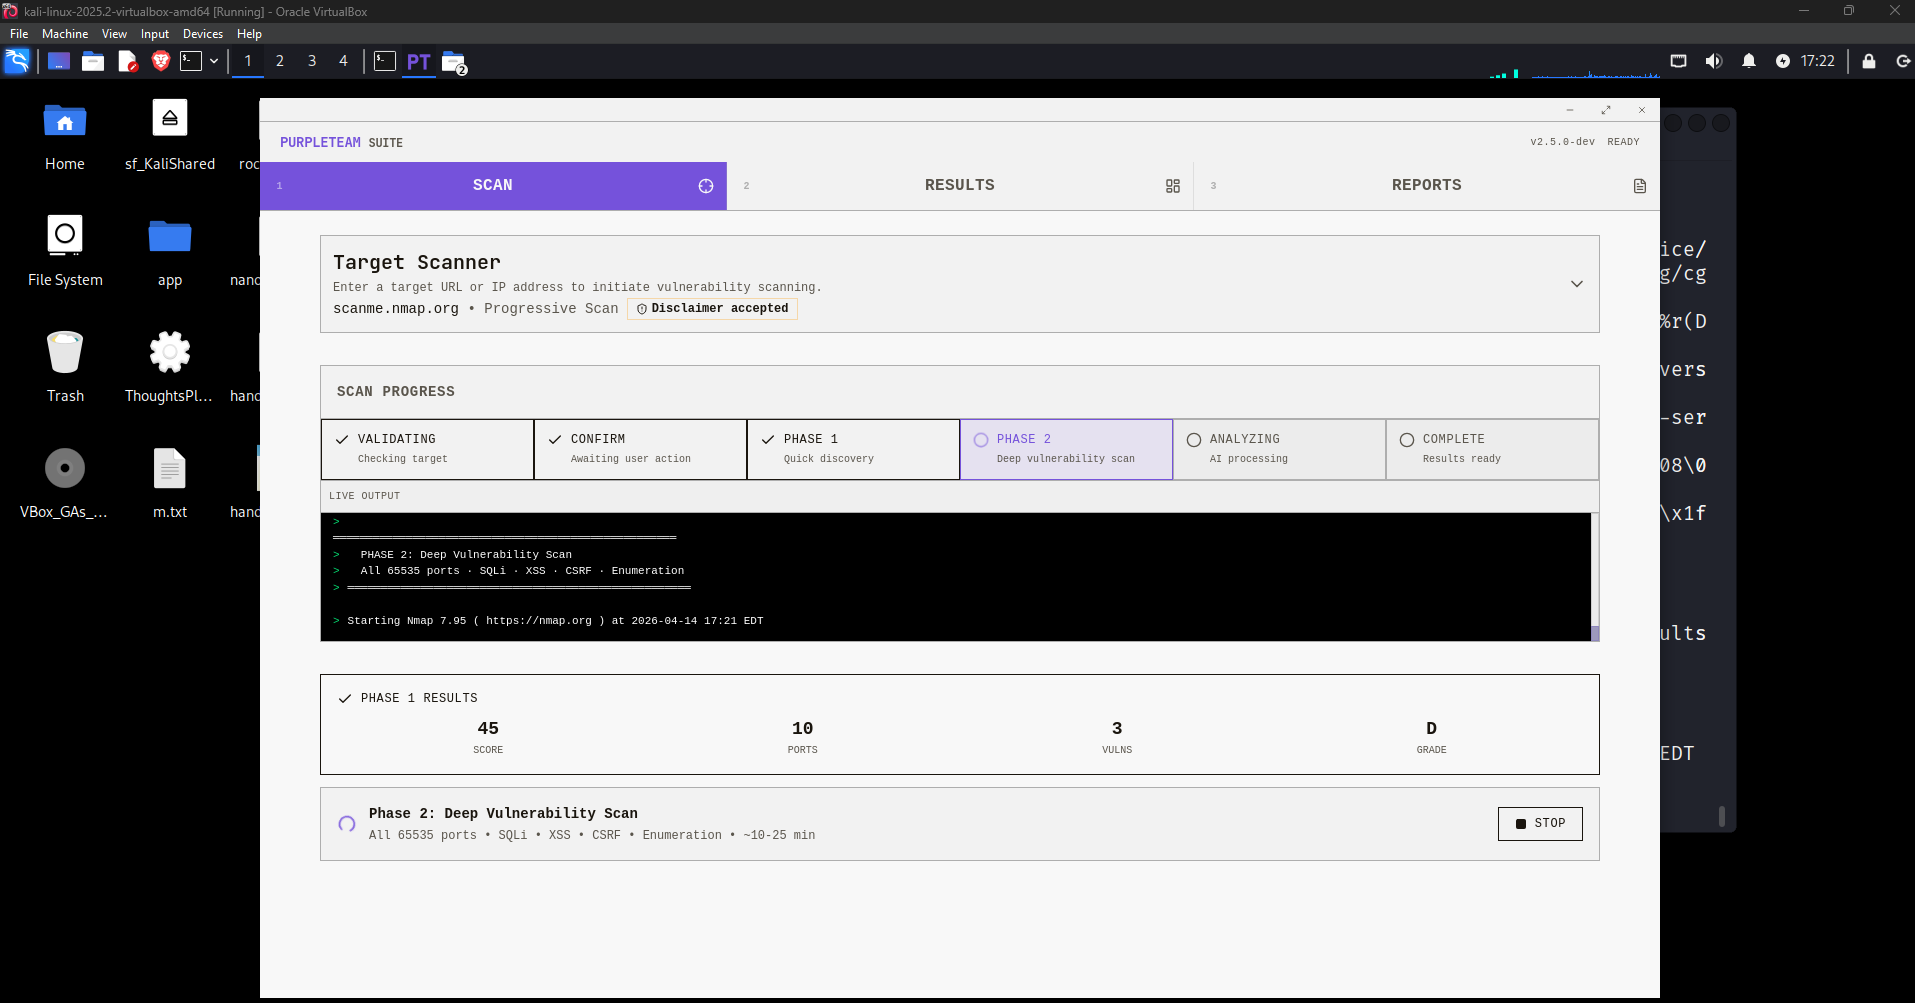
\includegraphics[width=\textwidth, height=0.82\textheight, keepaspectratio]{OS/Kali}
\caption{PurpleTeam Suite running on Kali Linux.}
\label{fig:kali-proof}
\end{figure}

\begin{figure}[H]
\centering
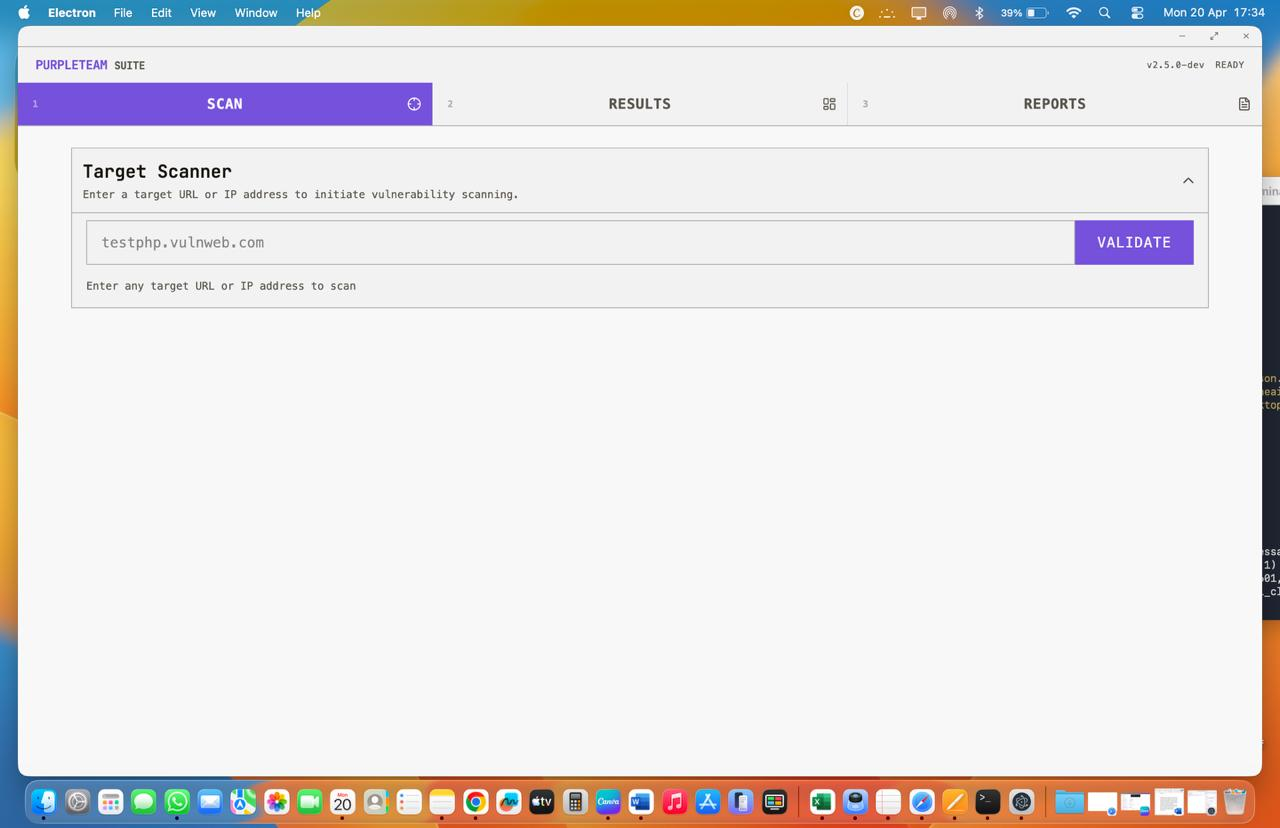
\includegraphics[width=\textwidth, height=0.82\textheight, keepaspectratio]{OS/MacOS}
\caption{PurpleTeam Suite running on macOS.}
\label{fig:macos-proof}
\end{figure}

\begin{table}[H]
\centering
\caption{Repository statistics at time of submission.}
\small
\begin{tabularx}{\textwidth}{>{\raggedright\arraybackslash}p{7cm}>{\raggedright\arraybackslash}X}
\toprule
\textbf{Metric} & \textbf{Value} \\
\midrule
Total source files (\texttt{.ts}/\texttt{.tsx}, excl.\ \texttt{node\_modules}) & 43 \\
Lines of TypeScript (estimated) & $\sim$10{,}500 \\
Pipeline modules & 10 (scanner, parser, OWASP mapper, scorer, LLM, hallucination guard, delta, reports, feature toggles, metrics) \\
Evaluation reports exported & 11 PDF files (\texttt{data/reports/}) \\
\bottomrule
\end{tabularx}
\end{table}

\chapter{Project Schedule}

\begin{figure}[H]
\centering
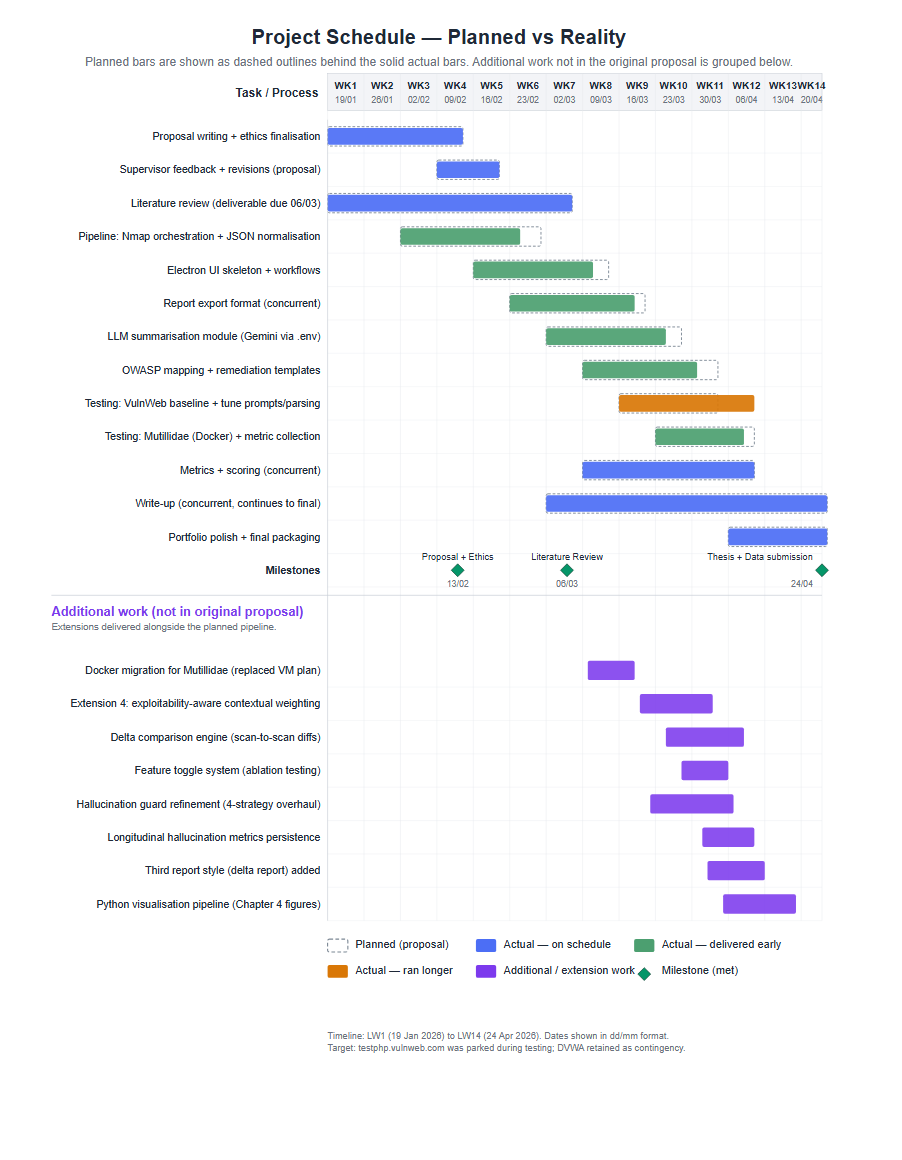
\includegraphics[width=\textwidth,height=0.78\textheight,keepaspectratio]{planned_vs_reality.png}
\caption{Planned versus actual project schedule.}
\label{fig:planned-vs-reality}
\end{figure}


\end{appendices}

\end{document}
